\chapter{2020 Near Detector Fit Results}\label{sec:2020Fit}

The results of the analysis are presented in this Chapter, starting with the nominal MC prediction and fit validations in Sections \ref{sec:nommc}, \ref{sec:llhscan}, \ref{sec:sigvar}, and \ref{sec:asimov}. The data fit is presented in \ref{sec:datafit}, and the posterior predictive distributions and p values are are shown in \ref{sec:postpred}. Results from fits with updated binnings are then compared in Section \ref{sec:newbin}.


\section{Nominal MC}\label{sec:nommc}

The event rates for each sample are shown in Table \ref{tab:nomrates}. The CC 0$\pi$ samples are consistently underestimated in the MC prediction by $\sim20\%$, the CC 1$\pi$ samples are overestimated by $\sim10\%$ for FHC and underestimated by $\sim5-10\%$ for RHC, and the CC Other samples are underestimated by $\sim20-30\%$. The differences to data are consistent across to the FGDs to $\sim2\%$. Overall, the MC prediction is $16\%$ lower than the observed data.

\begin{center}
\begin{table}
\center
\begin{tabular}{c||c|c|c|c}
\hline \hline
\textbf{Sample} & \textbf{Raw MC} & \textbf{Nominal MC} & \textbf{Data} & \textbf{Data/MC} \\
\hline
\hline
\textbf{FGD1 FHC $\nu$ CC 0$\pi$} & & 27951.1 & 33443 & 1.20 \\ 
\textbf{FGD1 FHC $\nu$ CC 1$\pi$} & & 8358.97 & 7713 & 0.92 \\ 
\textbf{FGD1 FHC $\nu$ CC Other} & & 7031.47 & 8026 & 1.14 \\ \hline
\textbf{FGD2 FHC $\nu$ CC 0$\pi$} & & 27556.2 & 33156 & 1.20 \\
\textbf{FGD2 FHC $\nu$ CC 1$\pi$} & & 6723.98 & 6281 & 0.93\\
\textbf{FGD2 FHC $\nu$ CC Other} & & 6454.68 & 7700 & 1.19 \\ \hline
\textbf{FGD1 RHC $\bar{\nu}$ CC 0$\pi$} & & 6980.48 & 8388 & 1.20\\
\textbf{FGD1 RHC $\bar{\nu}$ CC 1$\pi$} & & 668.897 & 698 & 1.04\\
\textbf{FGD1 RHC $\bar{\nu}$ CC Other} & & 1230.34 & 1472 & 1.20\\ \hline
\textbf{FGD2 RHC $\bar{\nu}$ CC 0$\pi$} & & 6771.47 & 8334 & 1.23\\
\textbf{FGD2 RHC $\bar{\nu}$ CC 1$\pi$} & & 603.301 & 650 & 1.08\\
\textbf{FGD2 RHC $\bar{\nu}$ CC Other} & & 1135.13 & 1335 & 1.18\\ \hline
\textbf{FGD1 RHC $\nu$ CC 0$\pi$} & & 2916.3 & 3594 & 1.23\\
\textbf{FGD1 RHC $\nu$ CC 1$\pi$} & & 1115.99 & 1111 & 1.00\\
\textbf{FGD1 RHC $\nu$ CC Other} & & 1031.87 & 1344 & 1.30\\ \hline
\textbf{FGD2 RHC $\nu$ CC 0$\pi$} & & 2901.65 & 3433 & 1.18\\
\textbf{FGD2 RHC $\nu$ CC 1$\pi$} & & 898.111 & 926 & 1.03\\ 
\textbf{FGD2 RHC $\nu$ CC Other} & & 962.735 & 1245 & 1.29\\ \hline
\textbf{Total} & & 111293 & 128849 & 1.16\\ \hline\hline
\end{tabular}
\caption{MC and data event rates for the ND280 samples.}
\label{tab:nomrates}
\end{table}
\end{center}

The 2D nominal MC distributions are shown in Figure \ref{fig:2dnommc}. The uniform-rectangular binning described in Section \ref{sec:binning} is used for the initial fits. 


The projection of these distributions onto the $p_{\mu}$ axis are shown in Figure \ref{fig:pstack}, along with the data and interaction mode breakdown.

The CC 0$\pi$ and CC Other samples show oscillatory behaviour in the ratio of data to MC at low momentum. The ratio is consistently $>1$, but is slightly increased at the peak momentum for FHC and RHC $\nu$, and decreased at the peak for RHC $\bar{\nu}$. The ratio for the CC 1$\pi$ samples is more flat in momentum, but shows a small oscillation $<1$ at low momentum for FHC $\nu$, and $>1$ for RHC $\nu$ and $\bar{\nu}$. The behaviour is similar across the FGDs.

The FHC $\nu$ and RHC $\bar{\nu}$ CC 0$\pi$ samples are dominated by the target interaction modes CCQE and 2p2h. However, for RHC $\nu$, there is a large contamination of CC 1$\pi$ events. The FHC $\nu$ and RHC $\bar{\nu}$ CC 1$\pi$ samples are dominated by the target interaction modes CC 1$\pi$, CC coherent, and CC mult-$\pi$. For RHC $\nu$ the 1$\pi$ sample has a significant number of CC DIS events. The CC Other samples are populated by mainly the target interaction modes CC DIS, CC mult-$\pi$, and CC miscellaneous, but with a significant number CC $1\pi$ and CC coherent events for FHC $\nu$ and RHC $\bar{\nu}$.

\begin{figure}
\centering
\begin{subfigure}{.35\textwidth}
  \centering
  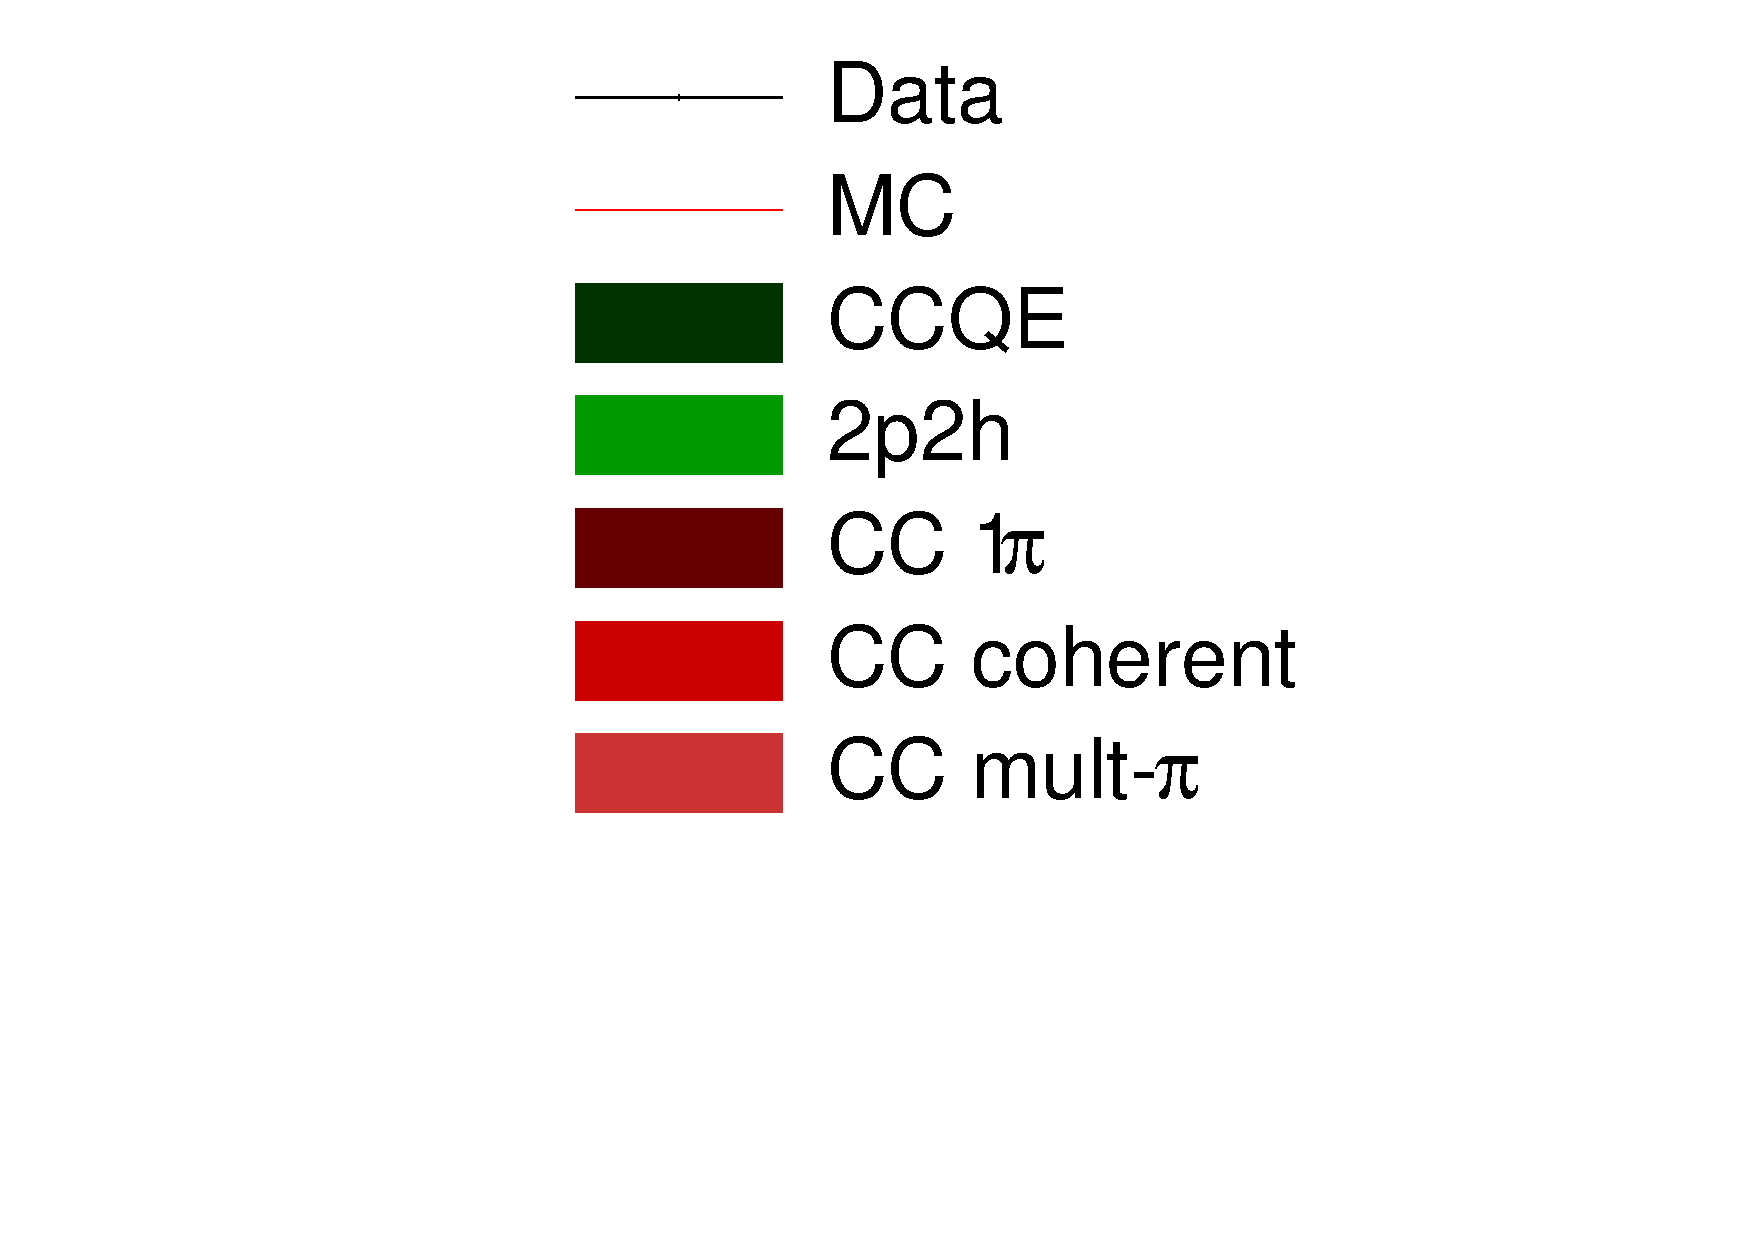
\includegraphics[width=0.7\linewidth]{figs/legend}
\end{subfigure}
\begin{subfigure}{.35\textwidth}
  \centering
  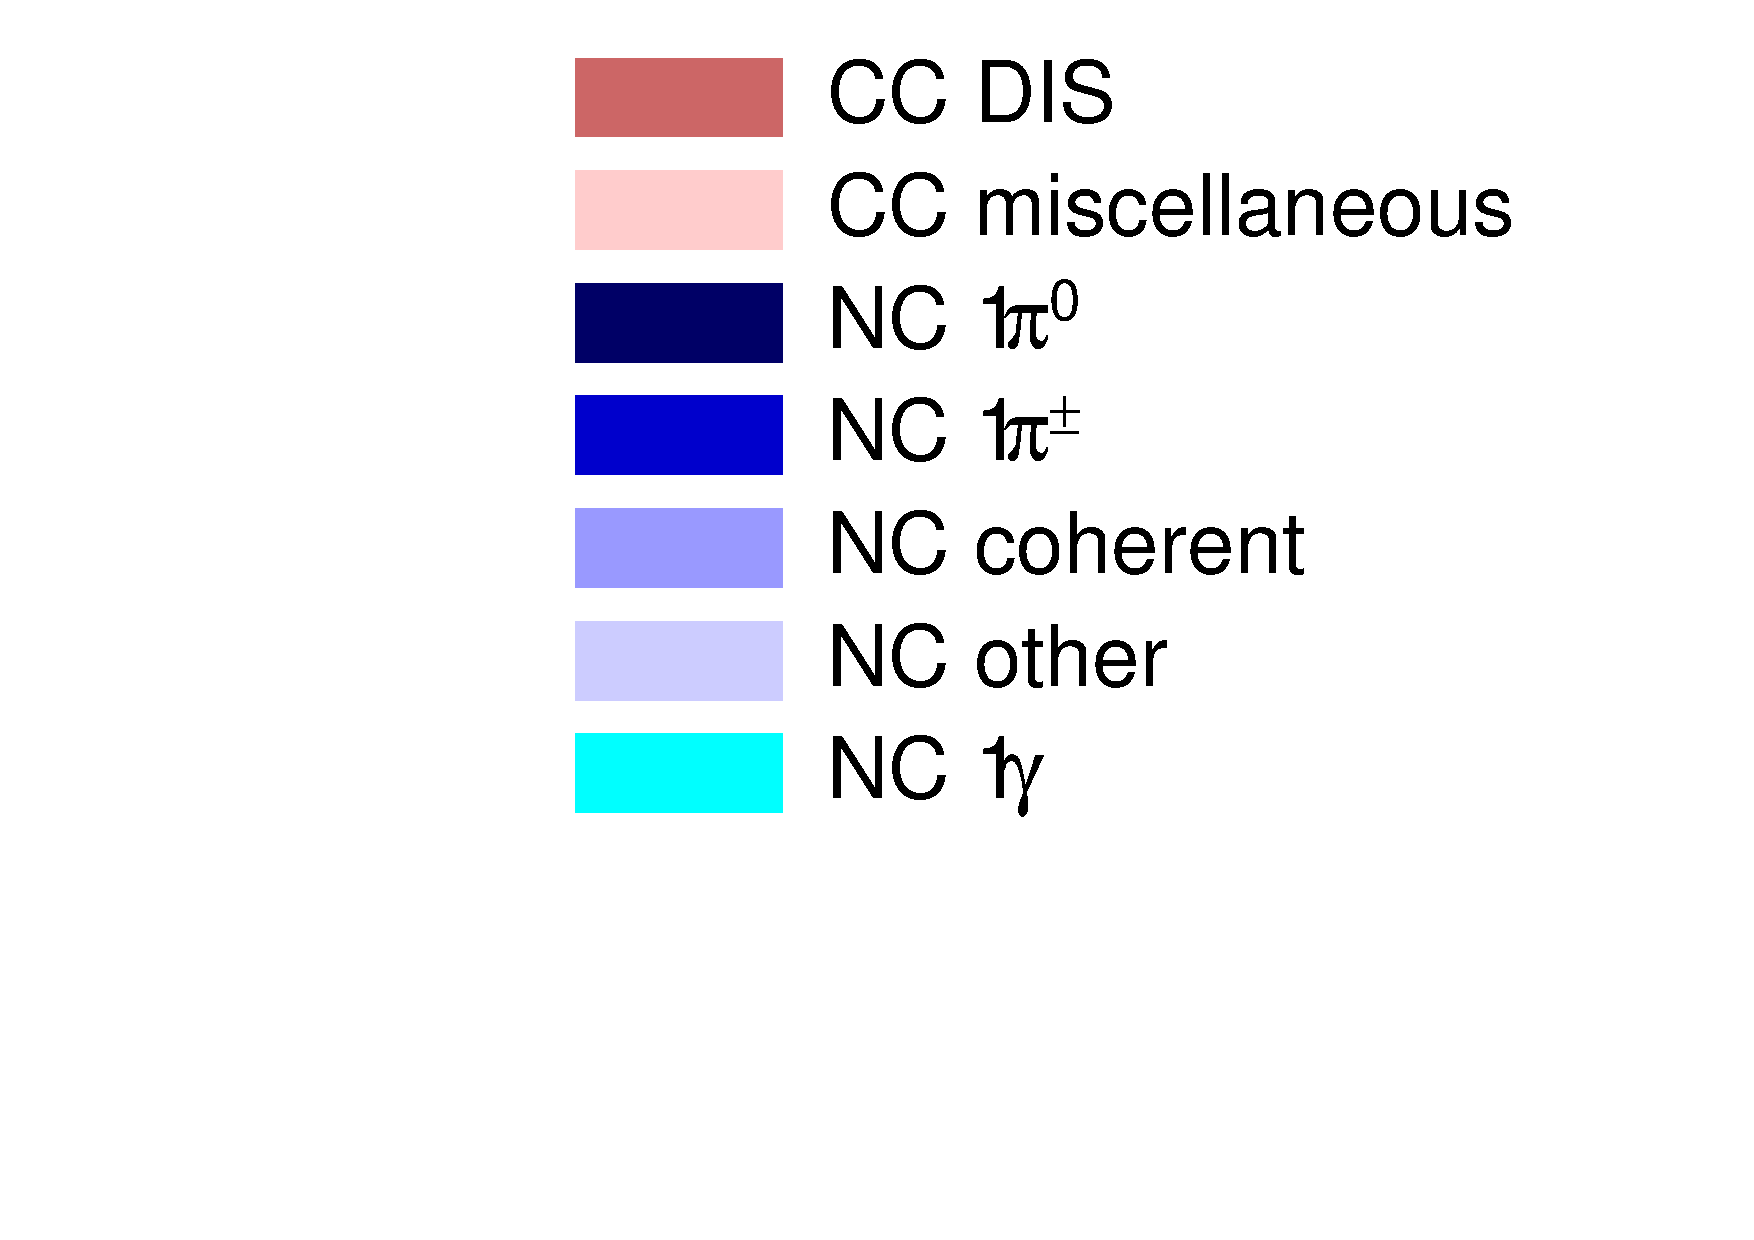
\includegraphics[width=0.7\linewidth]{figs/legend2}
\end{subfigure}
\begin{subfigure}{.32\textwidth}
  \centering
  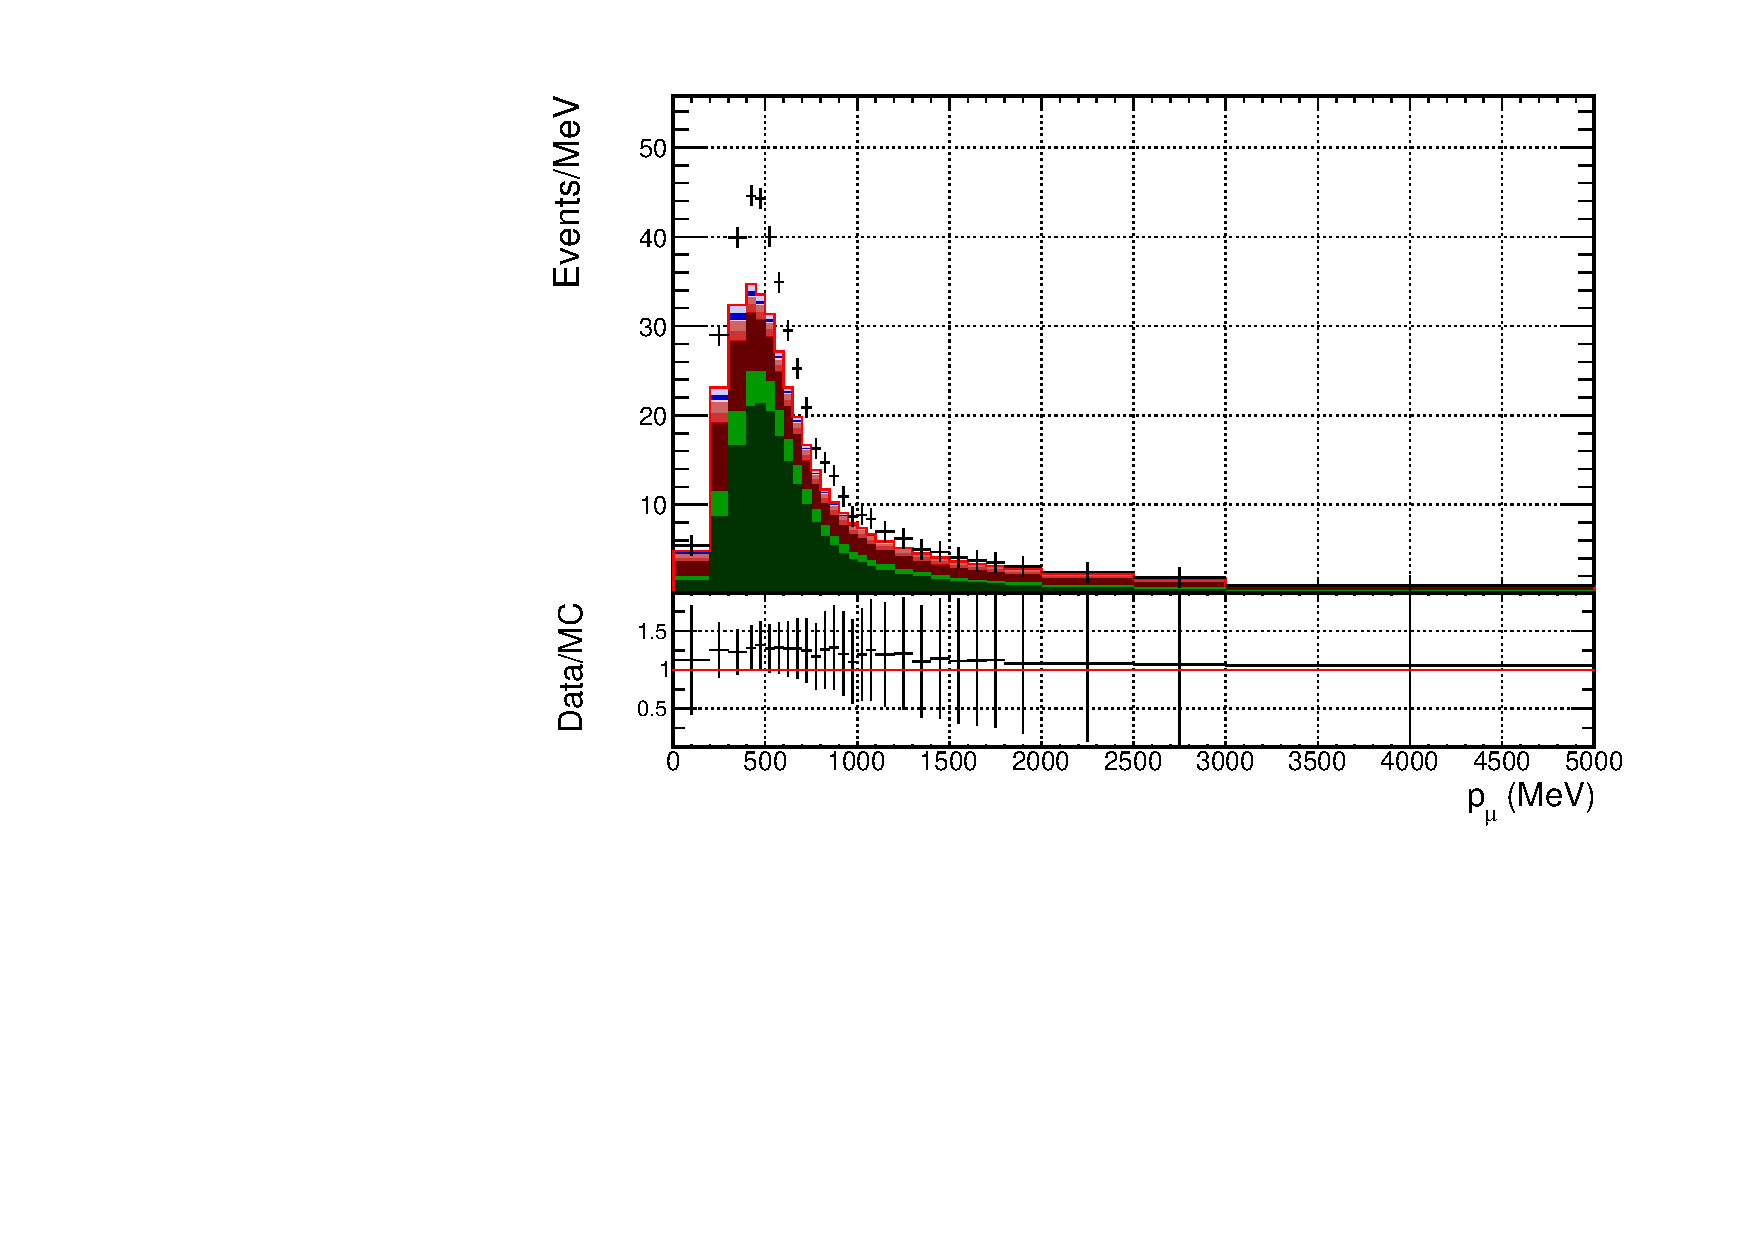
\includegraphics[width=0.95\linewidth]{figs/FGD2_numuCC_0pi_p}
  \caption{FGD1 FHC $\nu_{\mu}$ 0$\pi$}
  \label{fig:pstack_FGD1_numuCC_0pi}
\end{subfigure}
\begin{subfigure}{.32\textwidth}
  \centering
  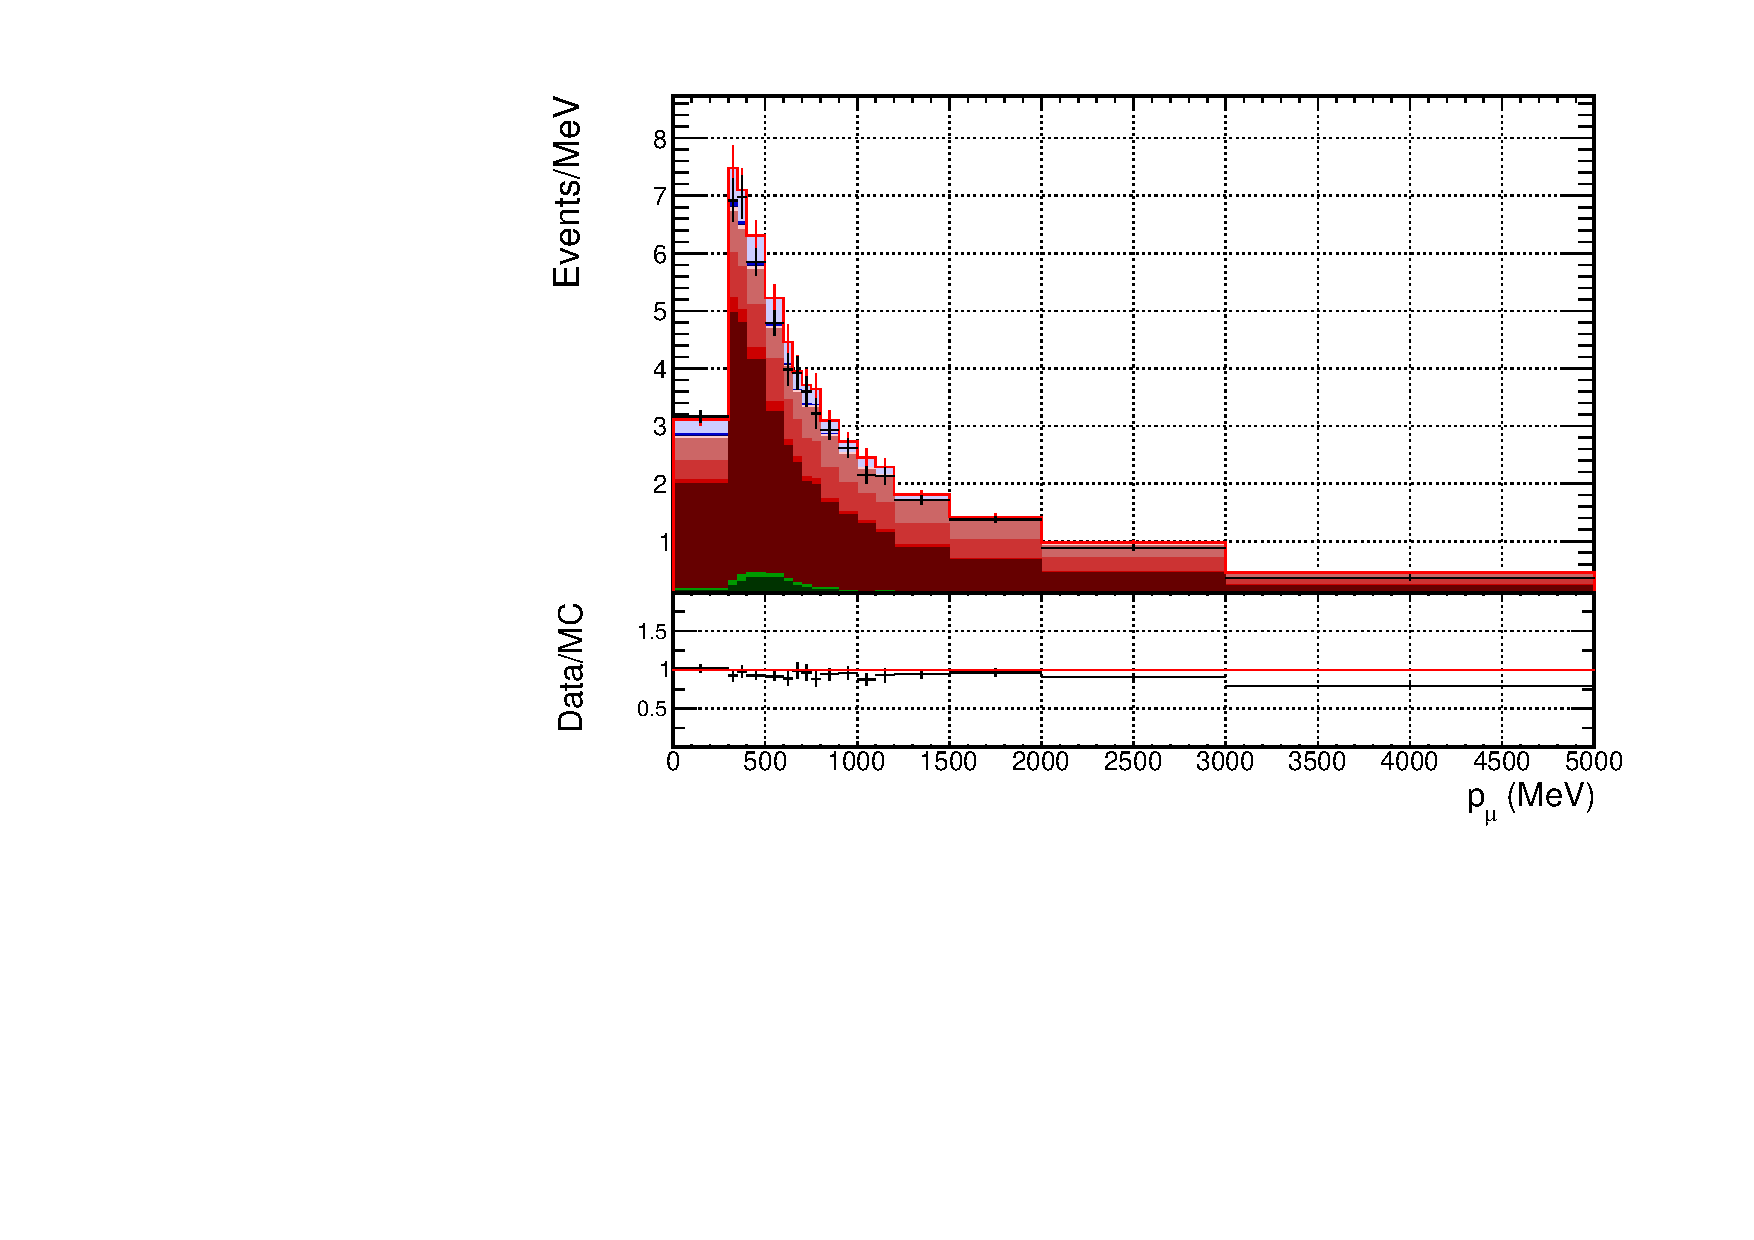
\includegraphics[width=0.95\linewidth]{figs/FGD1_numuCC_1pi_p}
  \caption{FGD1 FHC $\nu_{\mu}$ 1$\pi$}
  \label{fig:pstack_FGD1_numuCC_1pi}
\end{subfigure}
\begin{subfigure}{.32\textwidth}
  \centering
  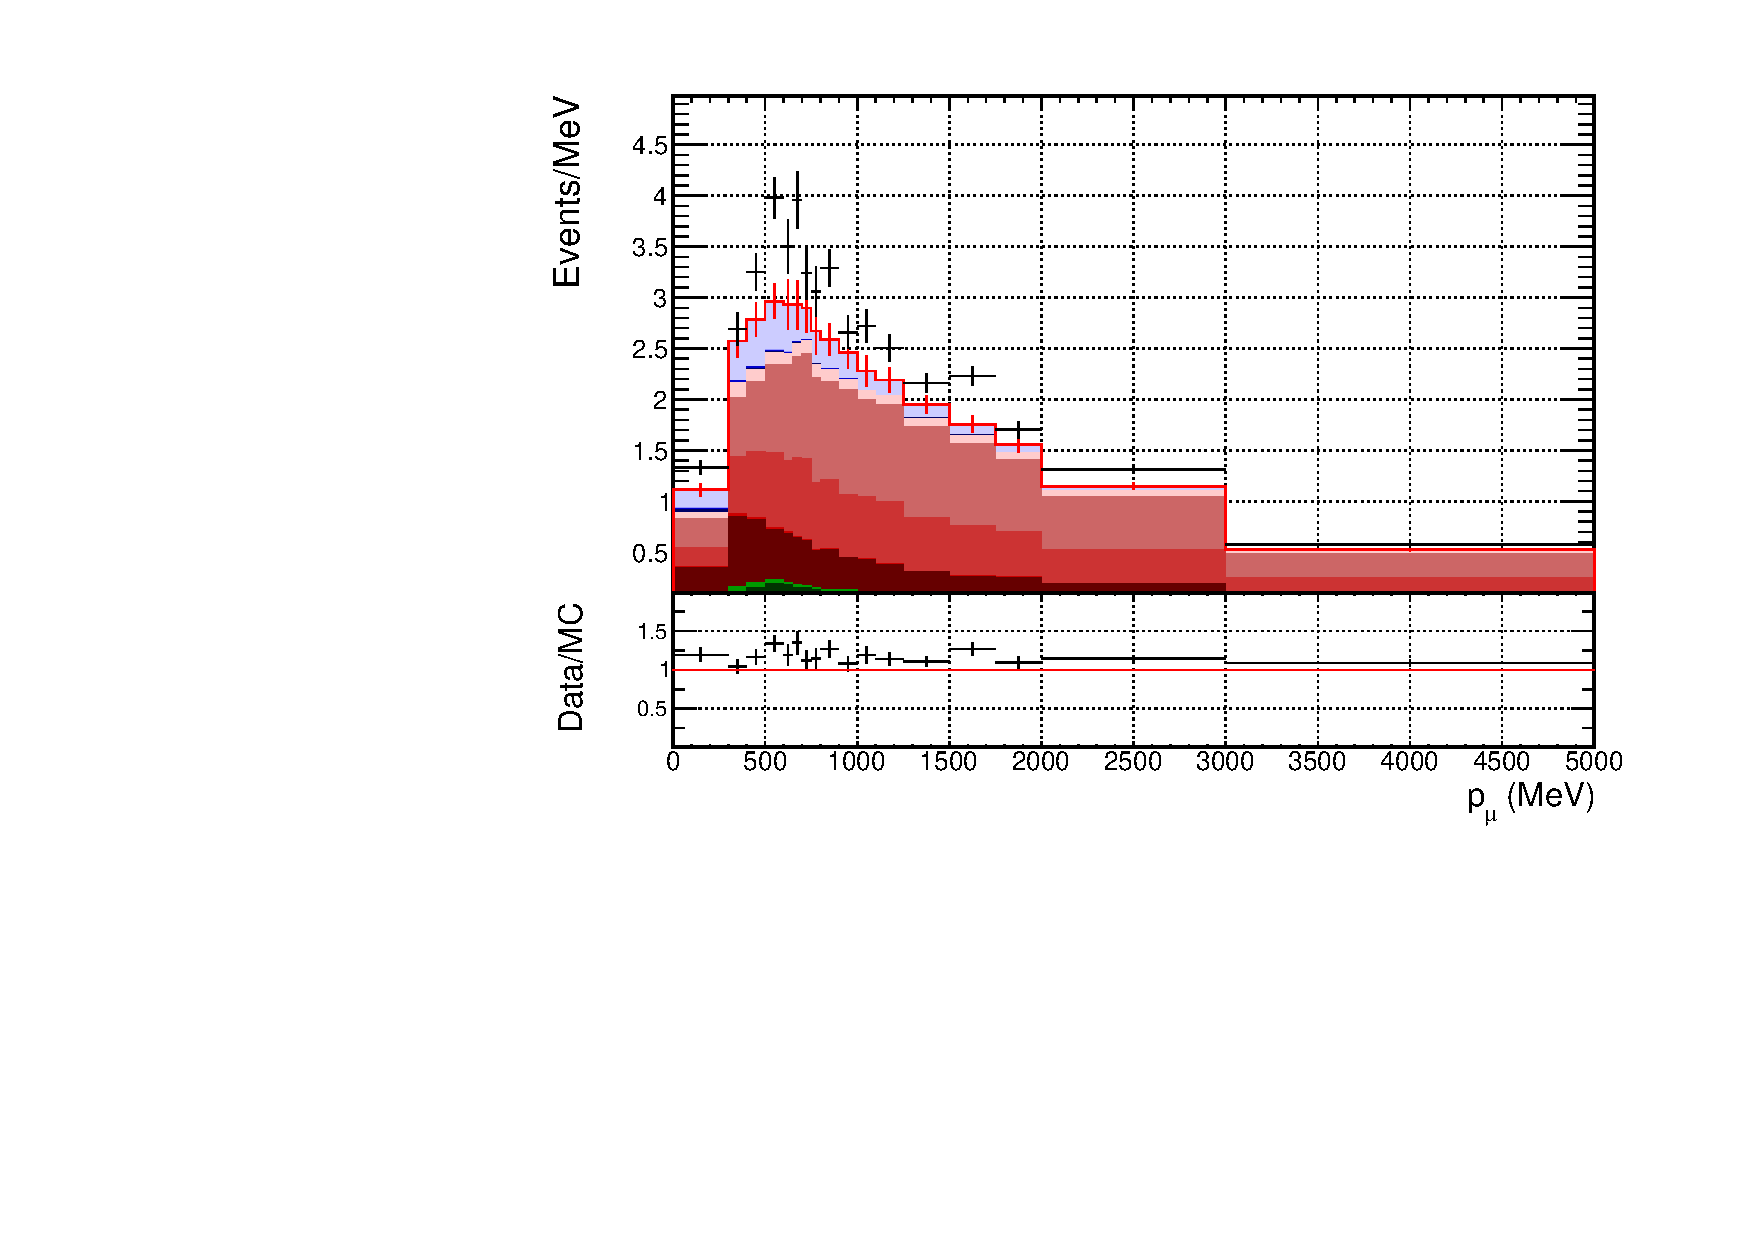
\includegraphics[width=0.95\linewidth]{figs/FGD1_numuCC_other_p}
  \caption{FGD1 FHC $\nu_{\mu}$ Other}
  \label{fig:pstack_FGD1_numuCC_other}
\end{subfigure}
\centering
\begin{subfigure}{.32\textwidth}
  \centering
  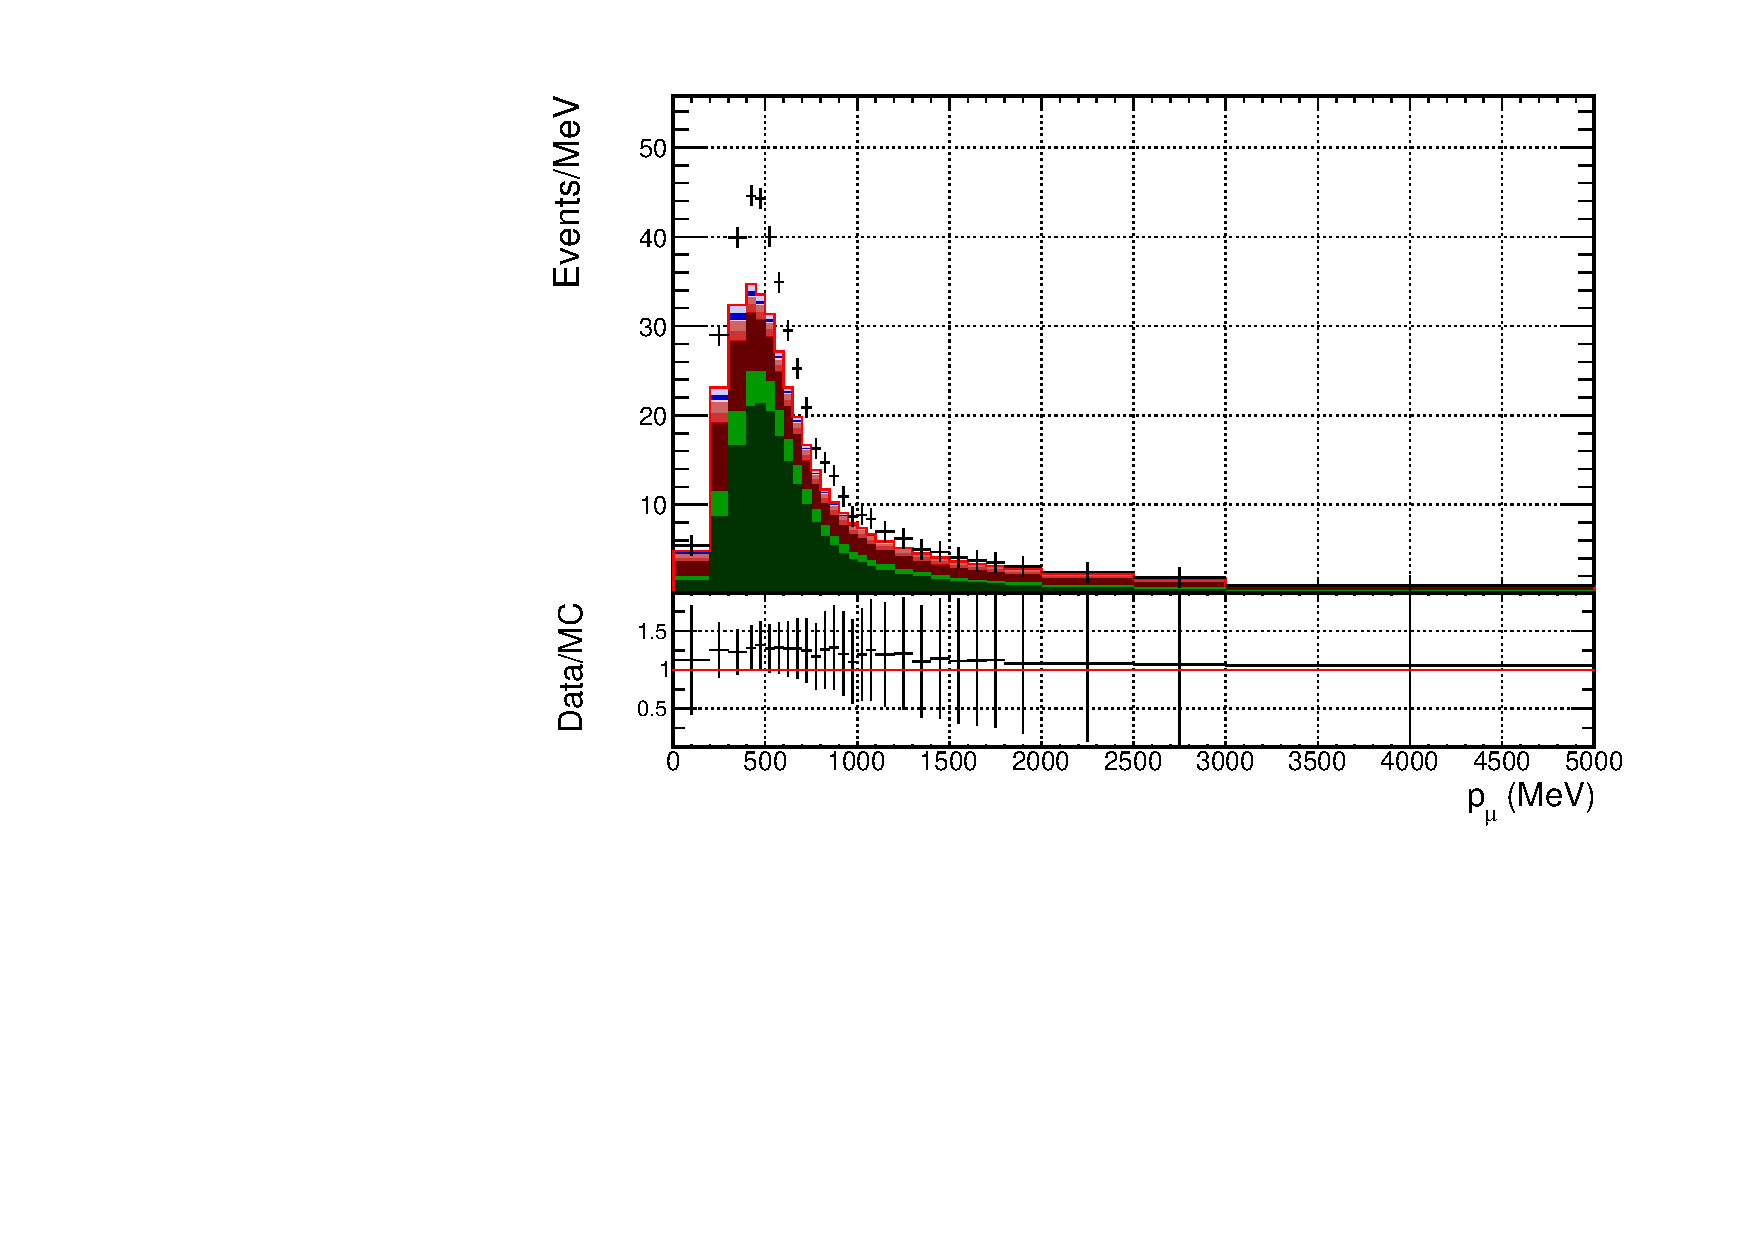
\includegraphics[width=0.95\linewidth]{figs/FGD2_numuCC_0pi_p}
  \caption{FGD2 FHC $\nu_{\mu}$ 0$\pi$}
  \label{fig:pstack_FGD2_numuCC_0pi}
\end{subfigure}
\begin{subfigure}{.32\textwidth}
  \centering
  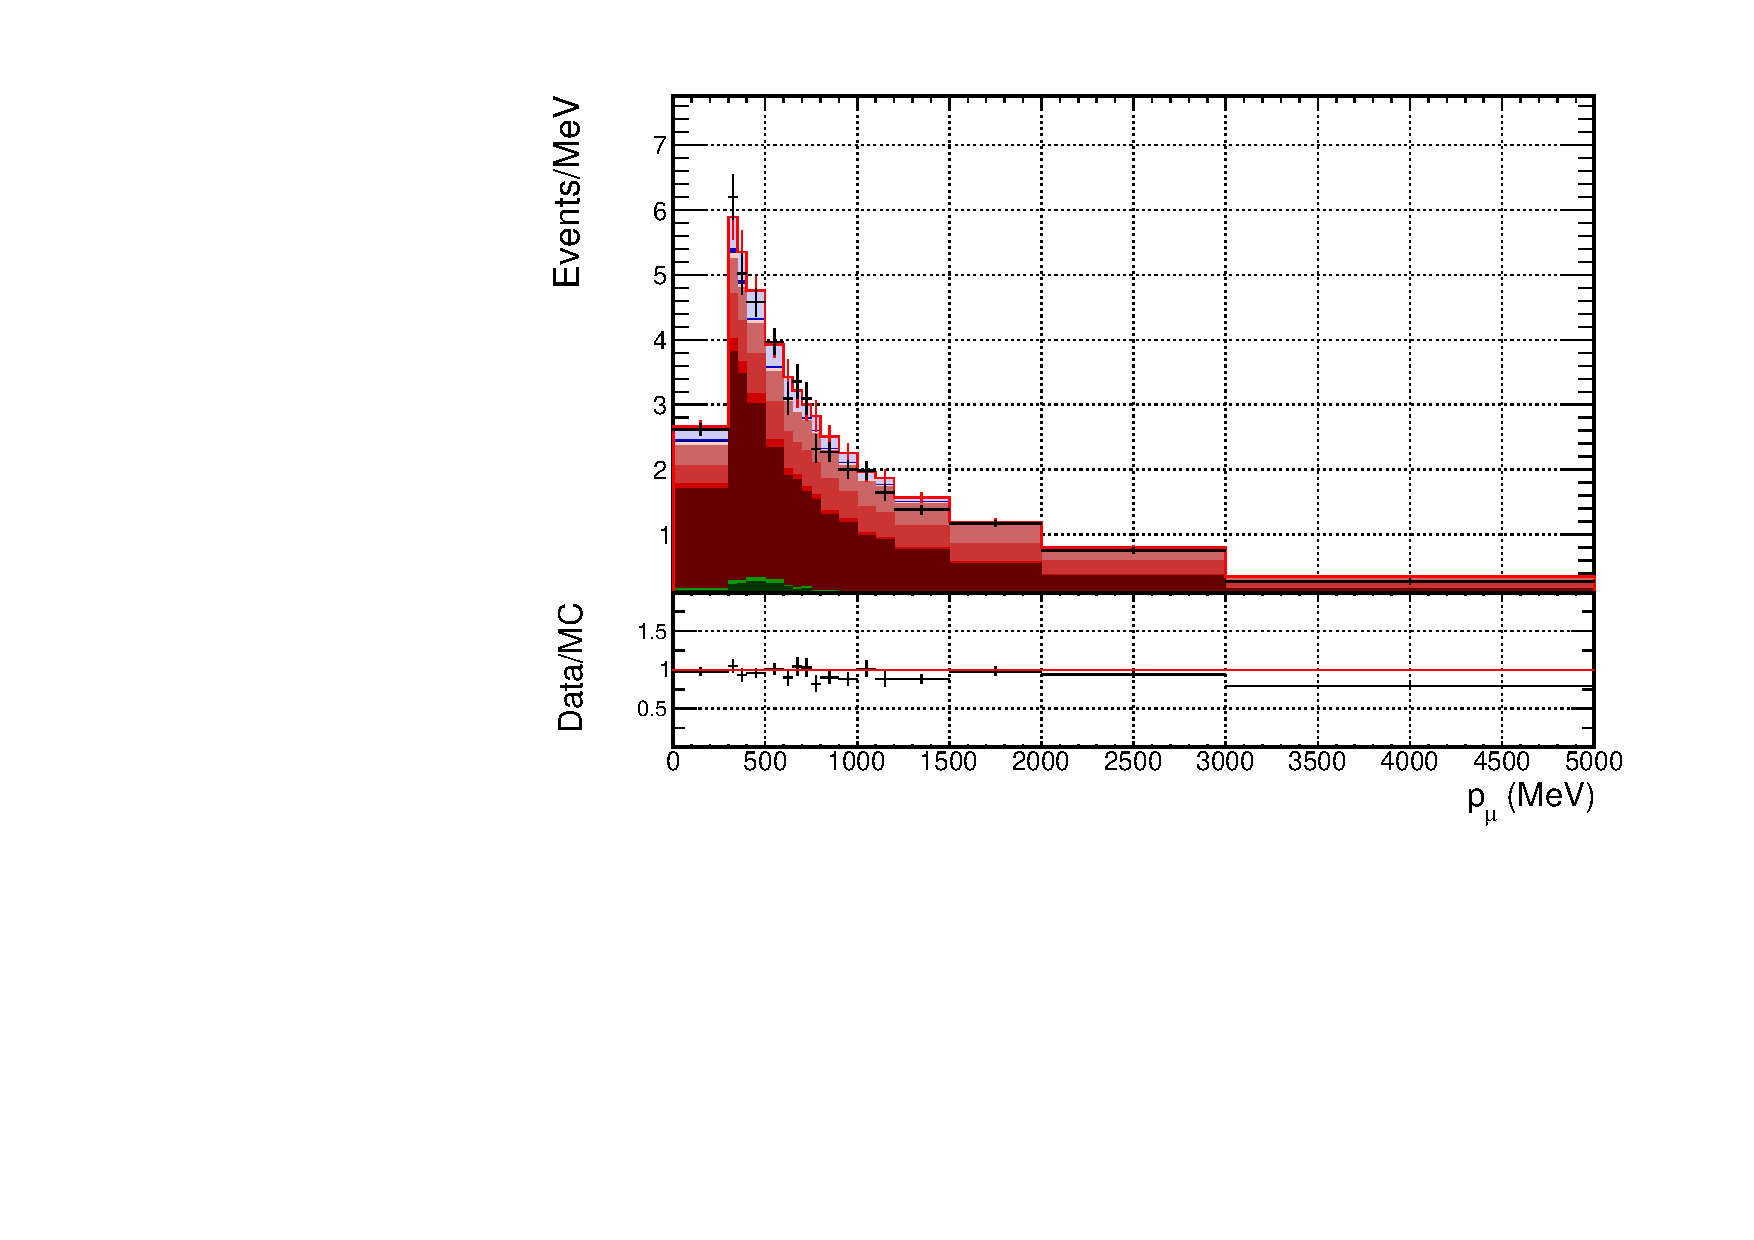
\includegraphics[width=0.95\linewidth]{figs/FGD2_numuCC_1pi_p}
  \caption{FGD2 FHC $\nu_{\mu}$ 1$\pi$}
  \label{fig:pstack_FGD2_numuCC_1pi}
\end{subfigure}
\begin{subfigure}{.32\textwidth}
  \centering
  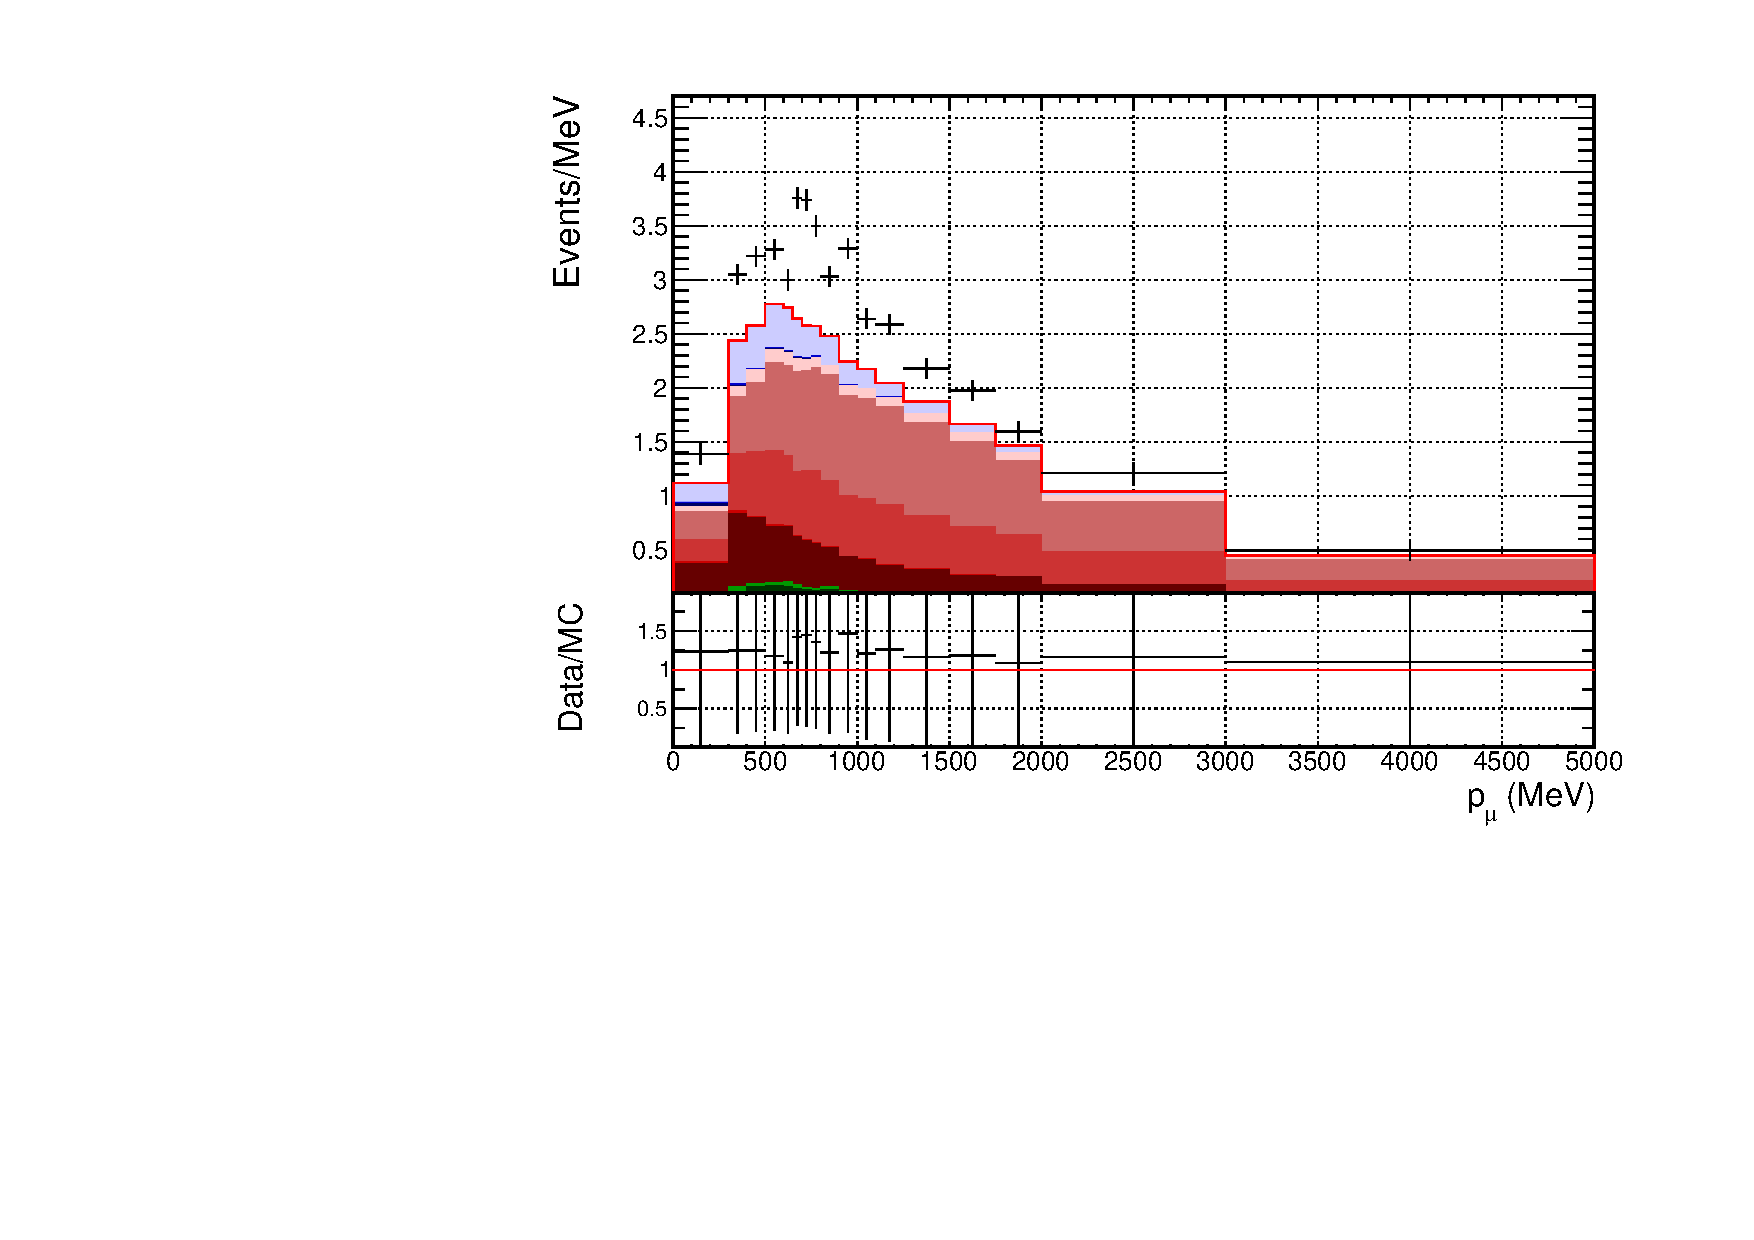
\includegraphics[width=0.95\linewidth]{figs/FGD2_numuCC_other_p}
  \caption{FGD2 $\nu_{\mu}$ Other}
  \label{fig:pstack_FGD2_numuCC_other}
\end{subfigure}
\centering
\begin{subfigure}{.32\textwidth}
  \centering
  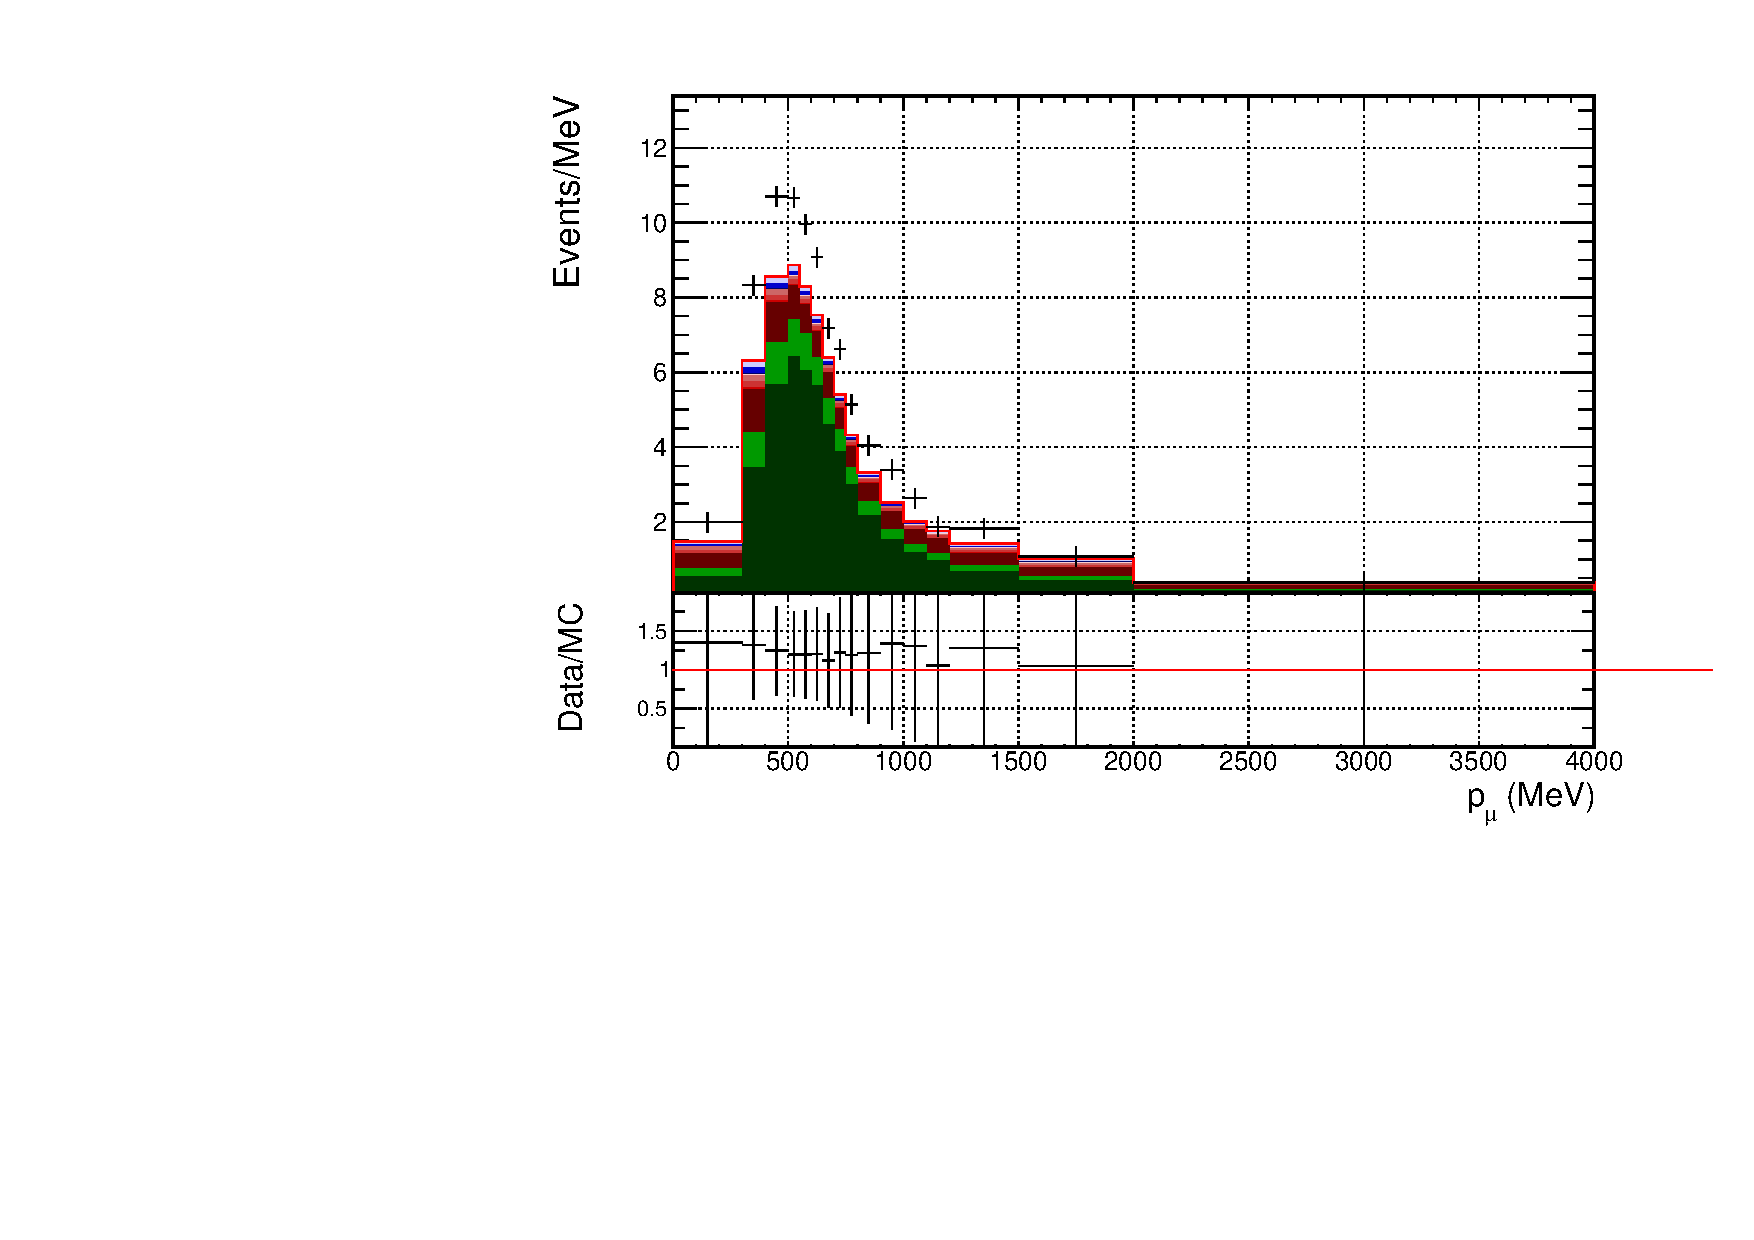
\includegraphics[width=0.95\linewidth]{figs/FGD1_anti-numuCC_0pi_p}
  \caption{FGD1 RHC $\bar{\nu_{\mu}}$ 0$\pi$}
  \label{fig:pstack_FGD1_anti-numuCC_0pi}
\end{subfigure}
\begin{subfigure}{.32\textwidth}
  \centering
  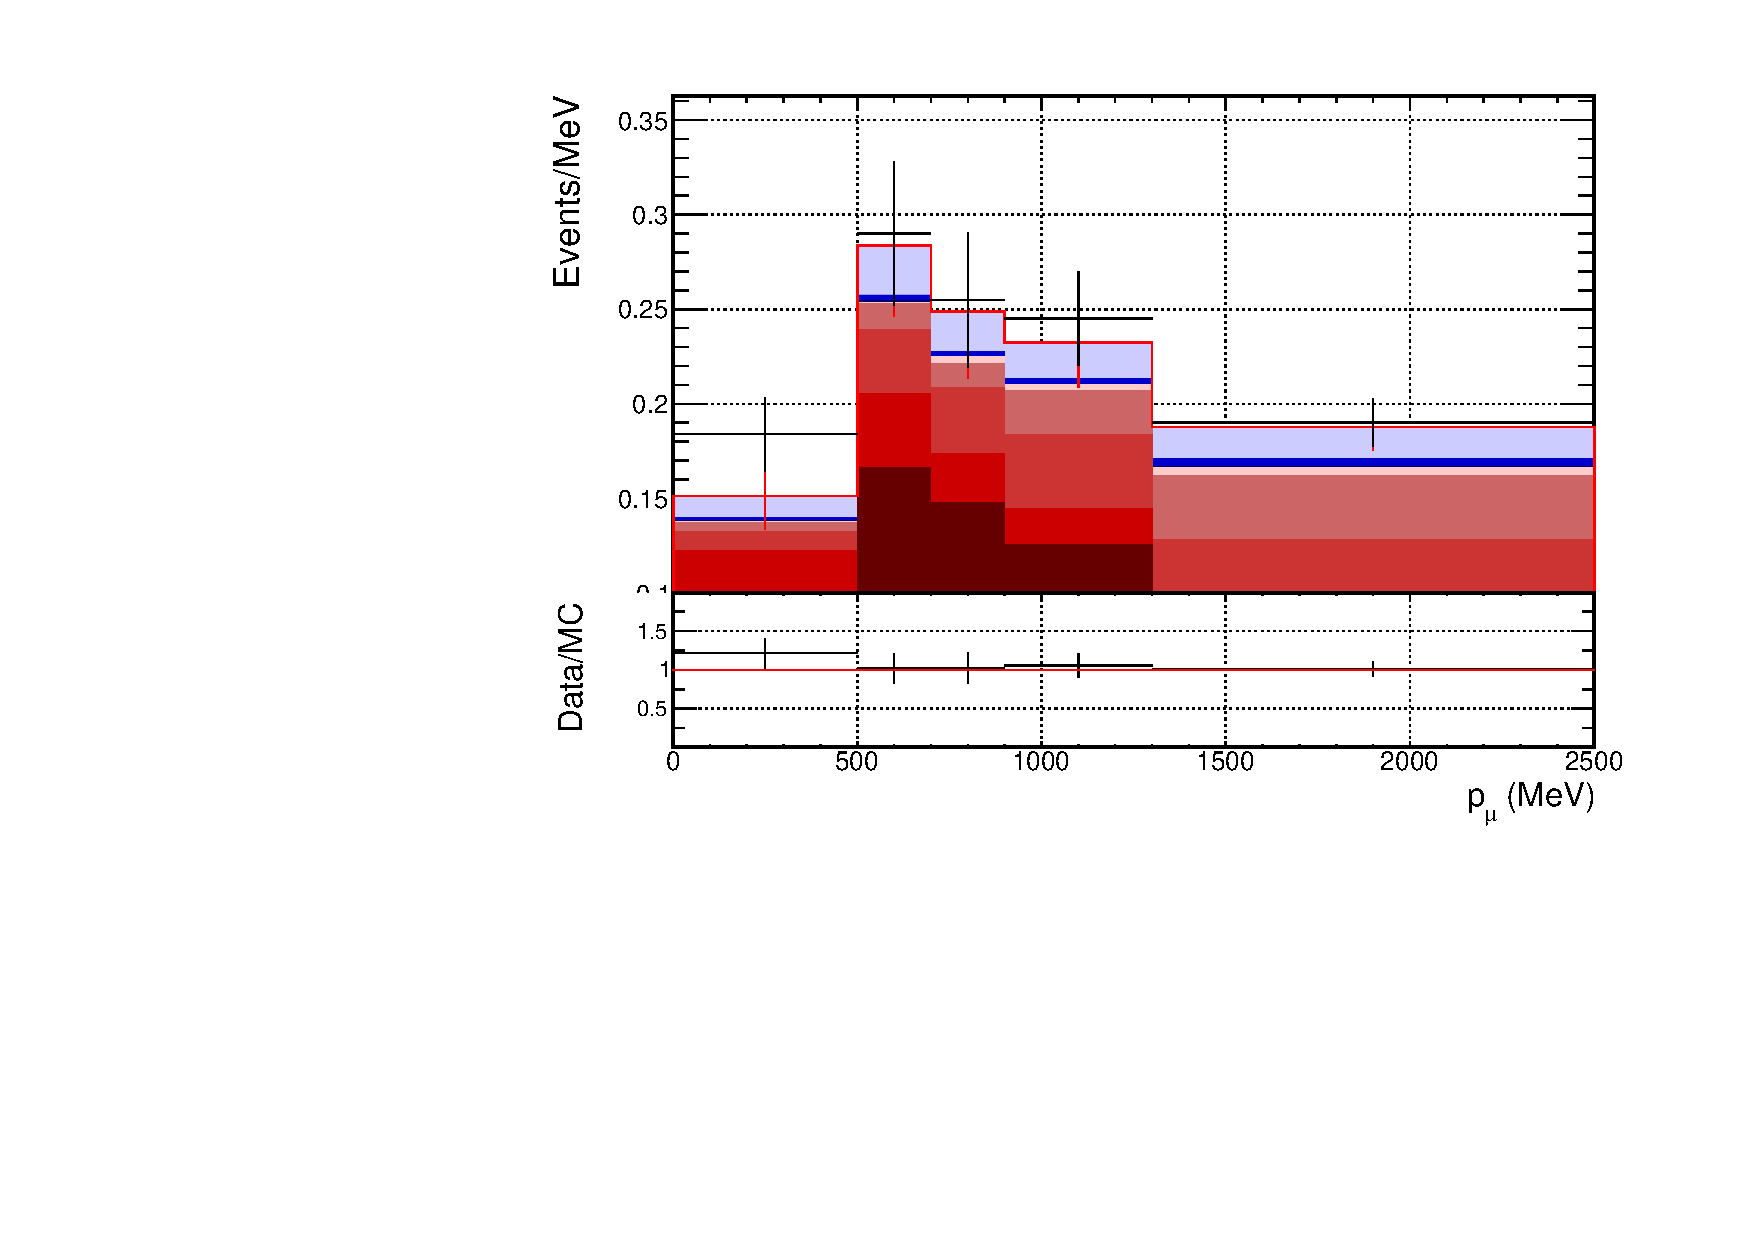
\includegraphics[width=0.95\linewidth]{figs/FGD1_anti-numuCC_1pi_p}
  \caption{FGD1 RHC $\bar{\nu_{\mu}}$ 1$\pi$}
  \label{fig:pstack_pstack_FGD1_anti-numuCC_1pi}
\end{subfigure}
\begin{subfigure}{.32\textwidth}
  \centering
  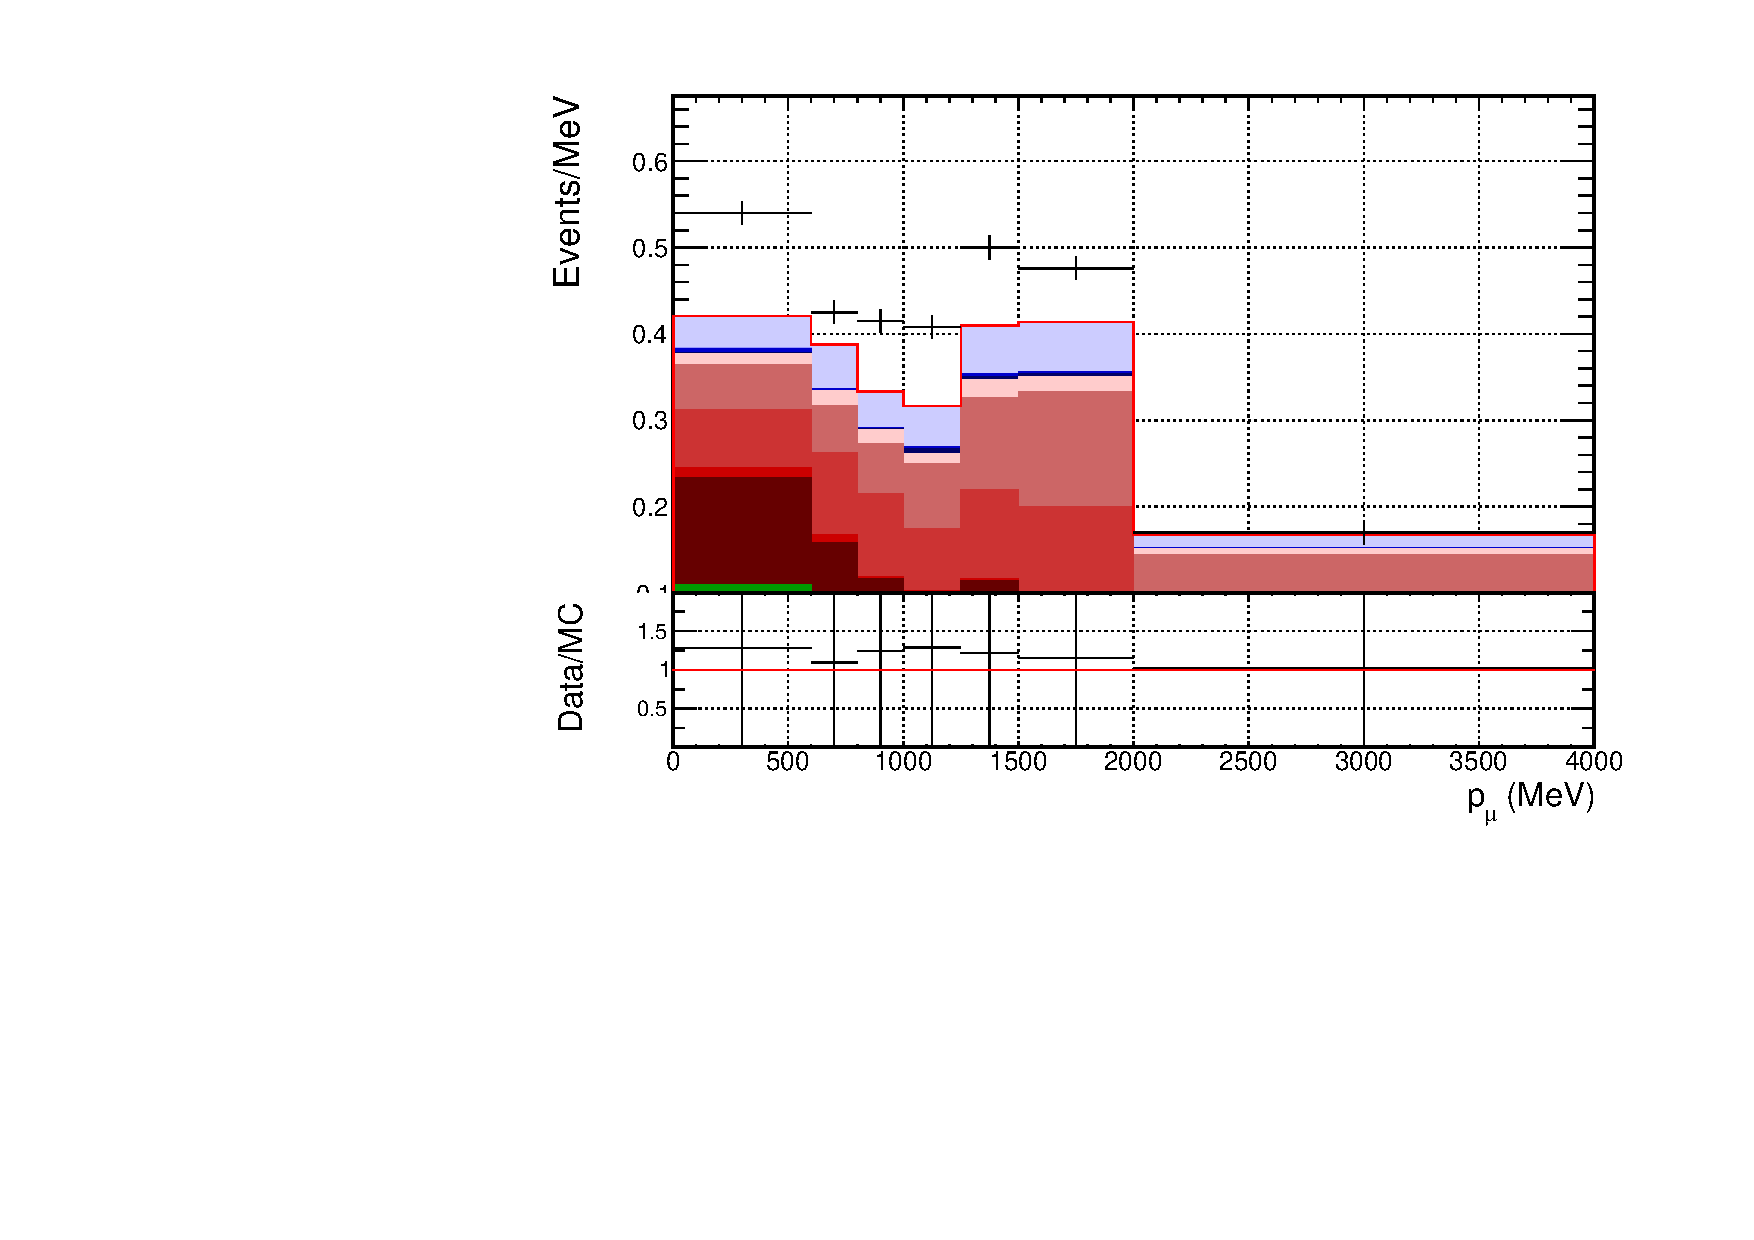
\includegraphics[width=0.95\linewidth]{figs/FGD1_anti-numuCC_other_p}
  \caption{FGD1 RHC $\bar{\nu_{\mu}}$ Other}
  \label{fig:pstack_FGD1_anti-numuCC_other}
\end{subfigure}
\centering
\begin{subfigure}{.32\textwidth}
  \centering
  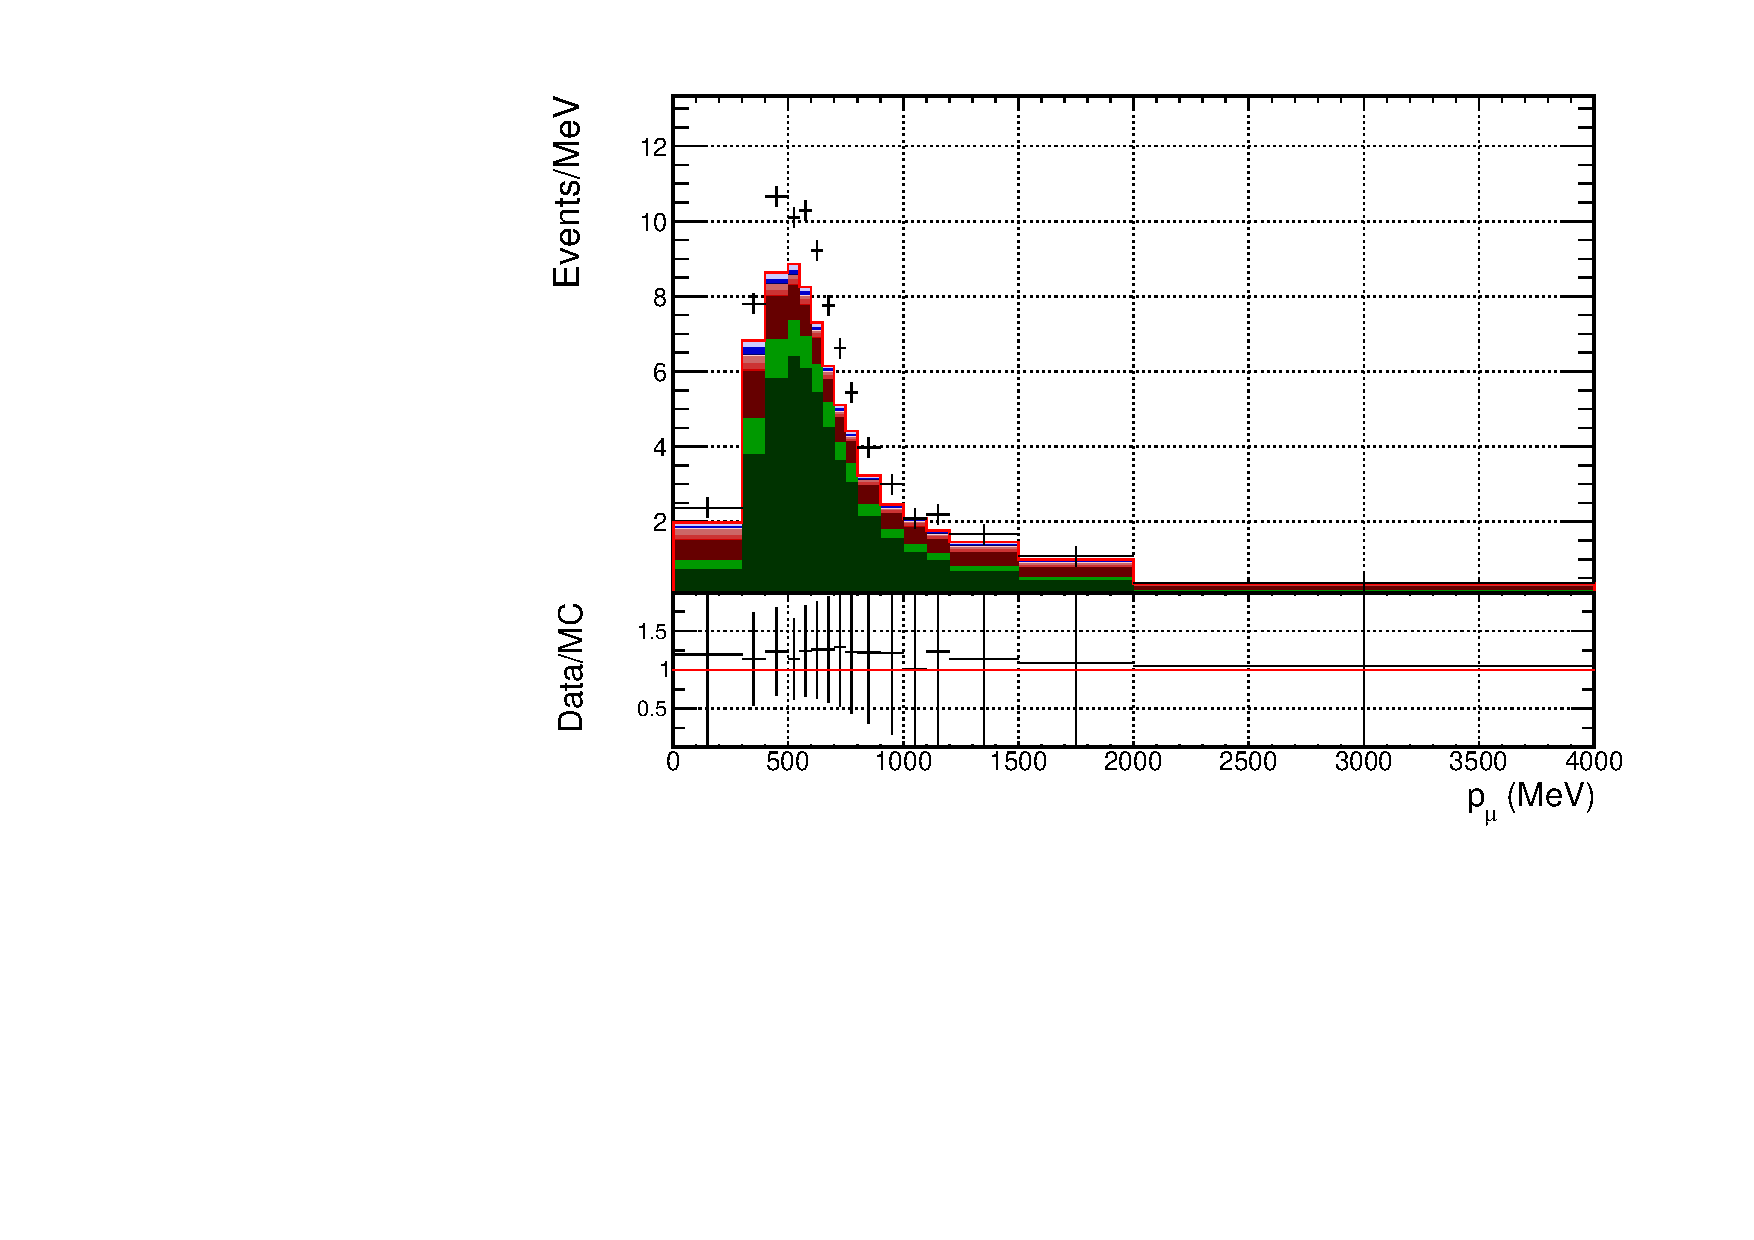
\includegraphics[width=0.95\linewidth]{figs/FGD2_anti-numuCC_0pi_p}
  \caption{FGD2 RHC $\bar{\nu_{\mu}}$ 0$\pi$}
  \label{fig:pstack_FGD2_anti-numuCC_0pi}
\end{subfigure}
\begin{subfigure}{.32\textwidth}
  \centering
  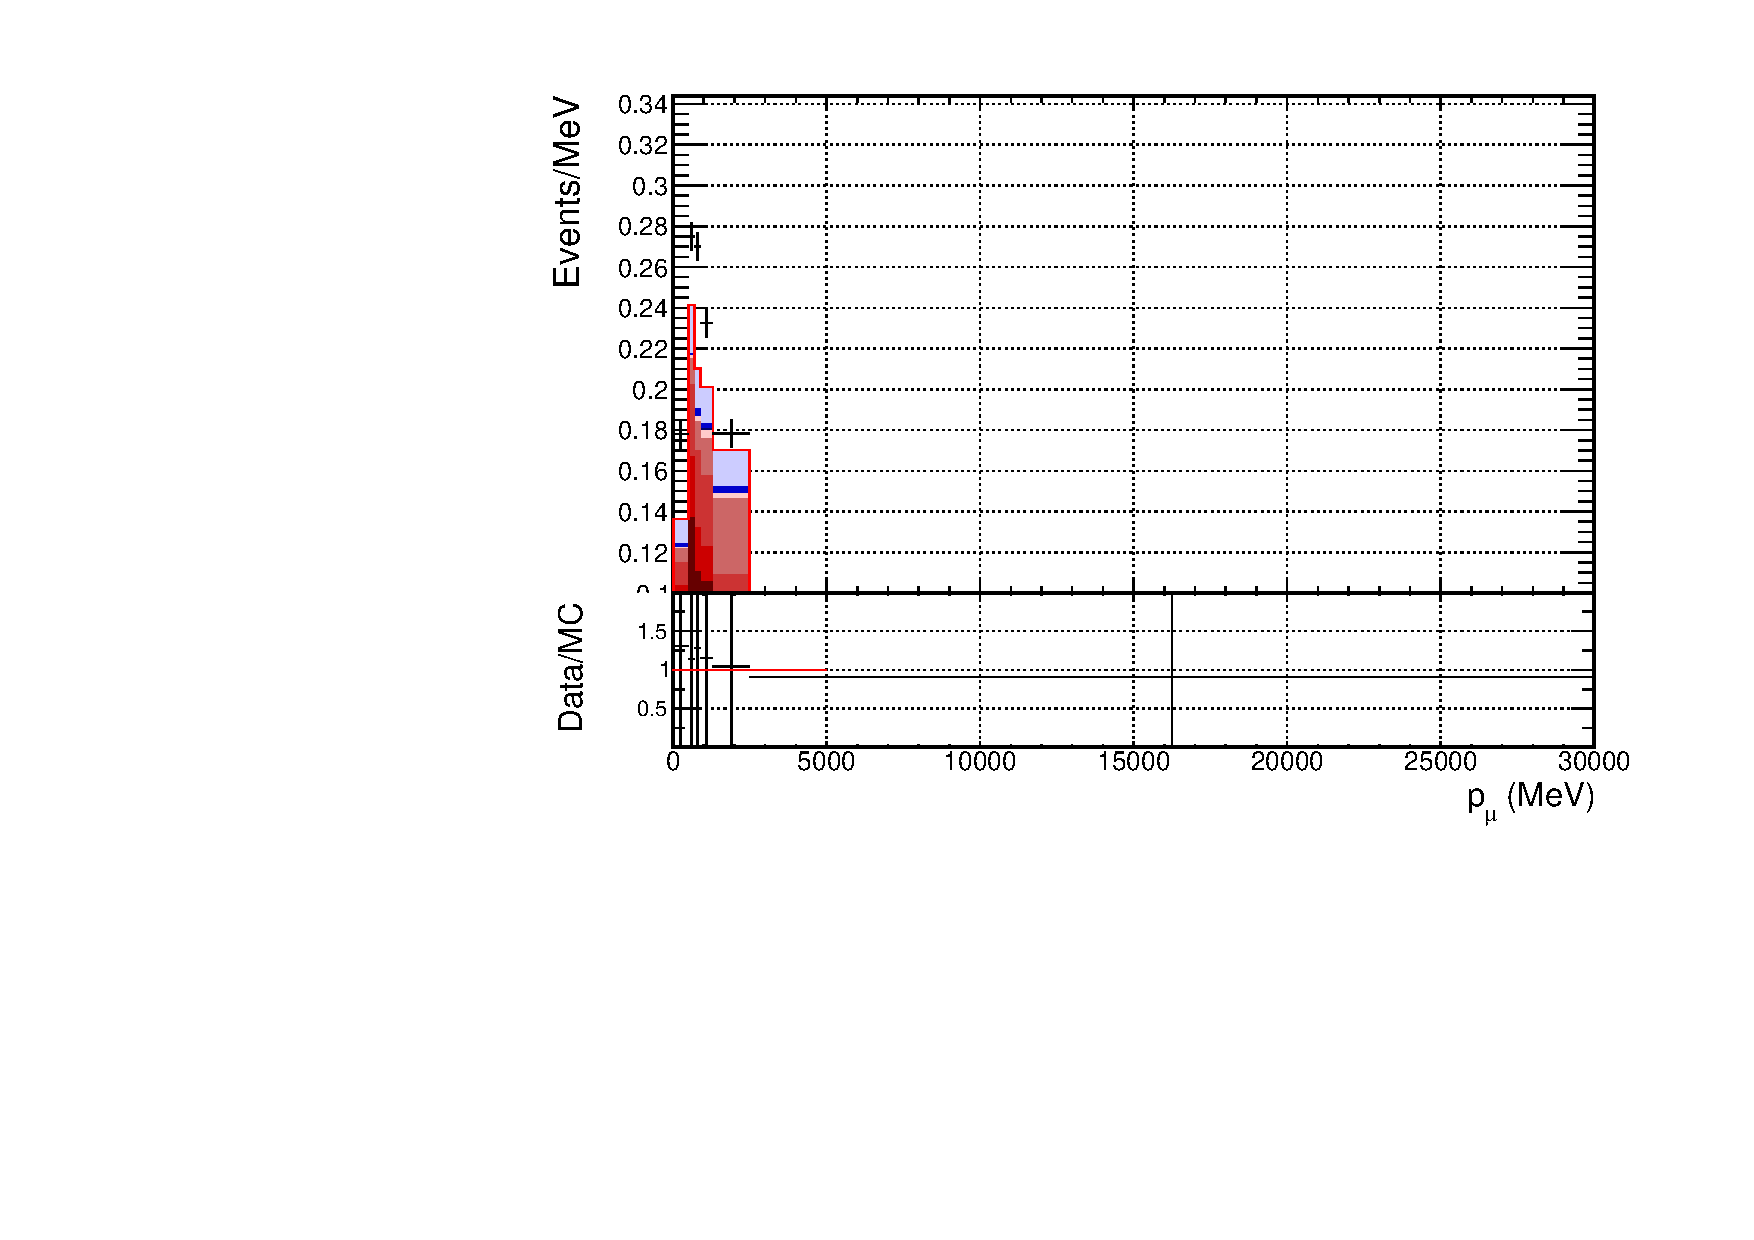
\includegraphics[width=0.95\linewidth]{figs/FGD2_anti-numuCC_1pi_p}
  \caption{FGD2 RHC $\bar{\nu_{\mu}}$ 1$\pi$}
  \label{fig:pstack_pstack_FGD2_anti-numuCC_1pi}
\end{subfigure}
\begin{subfigure}{.32\textwidth}
  \centering
  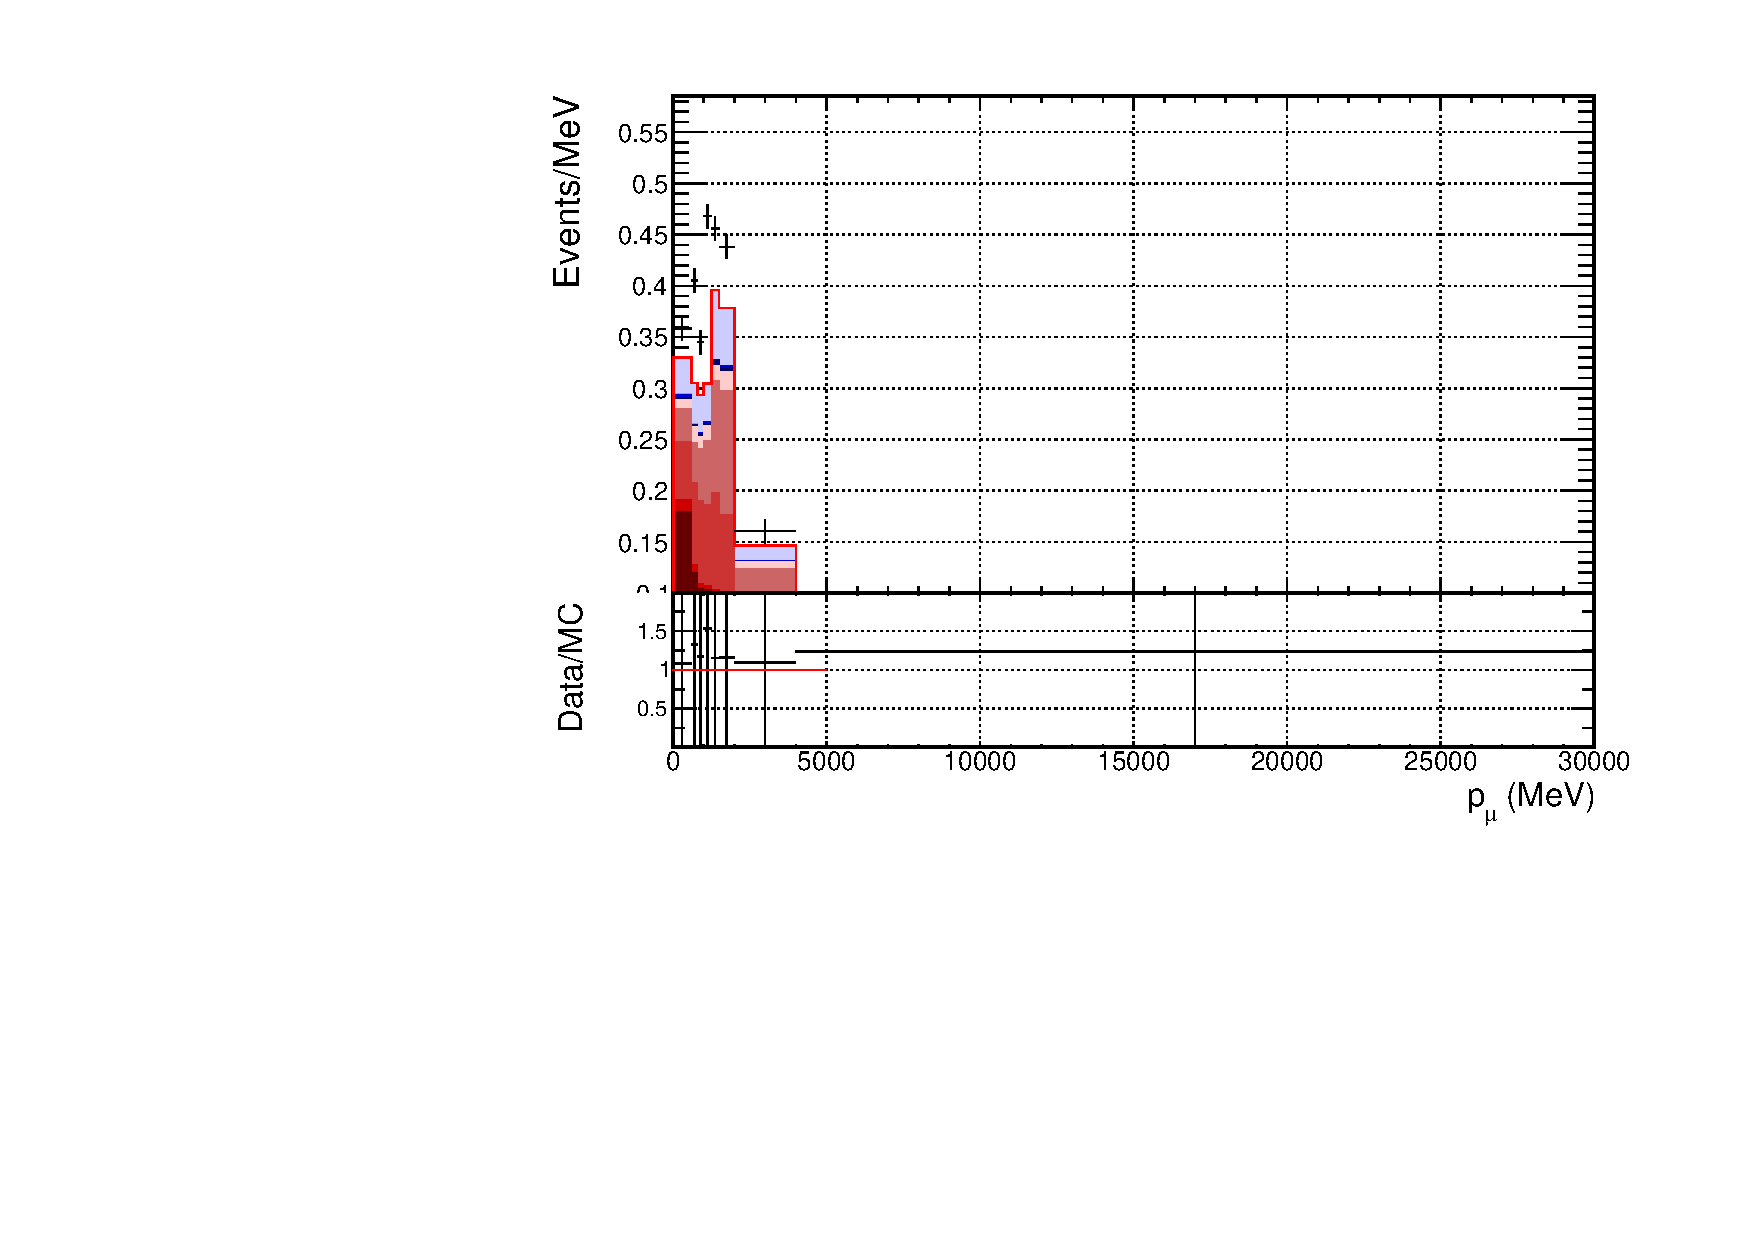
\includegraphics[width=0.95\linewidth]{figs/FGD2_anti-numuCC_other_p}
  \caption{FGD2 RHC $\bar{\nu_{\mu}}$ Other}
  \label{fig:pstack_FGD2_anti-numuCC_other}
\end{subfigure}
\begin{subfigure}{.32\textwidth}
  \centering
  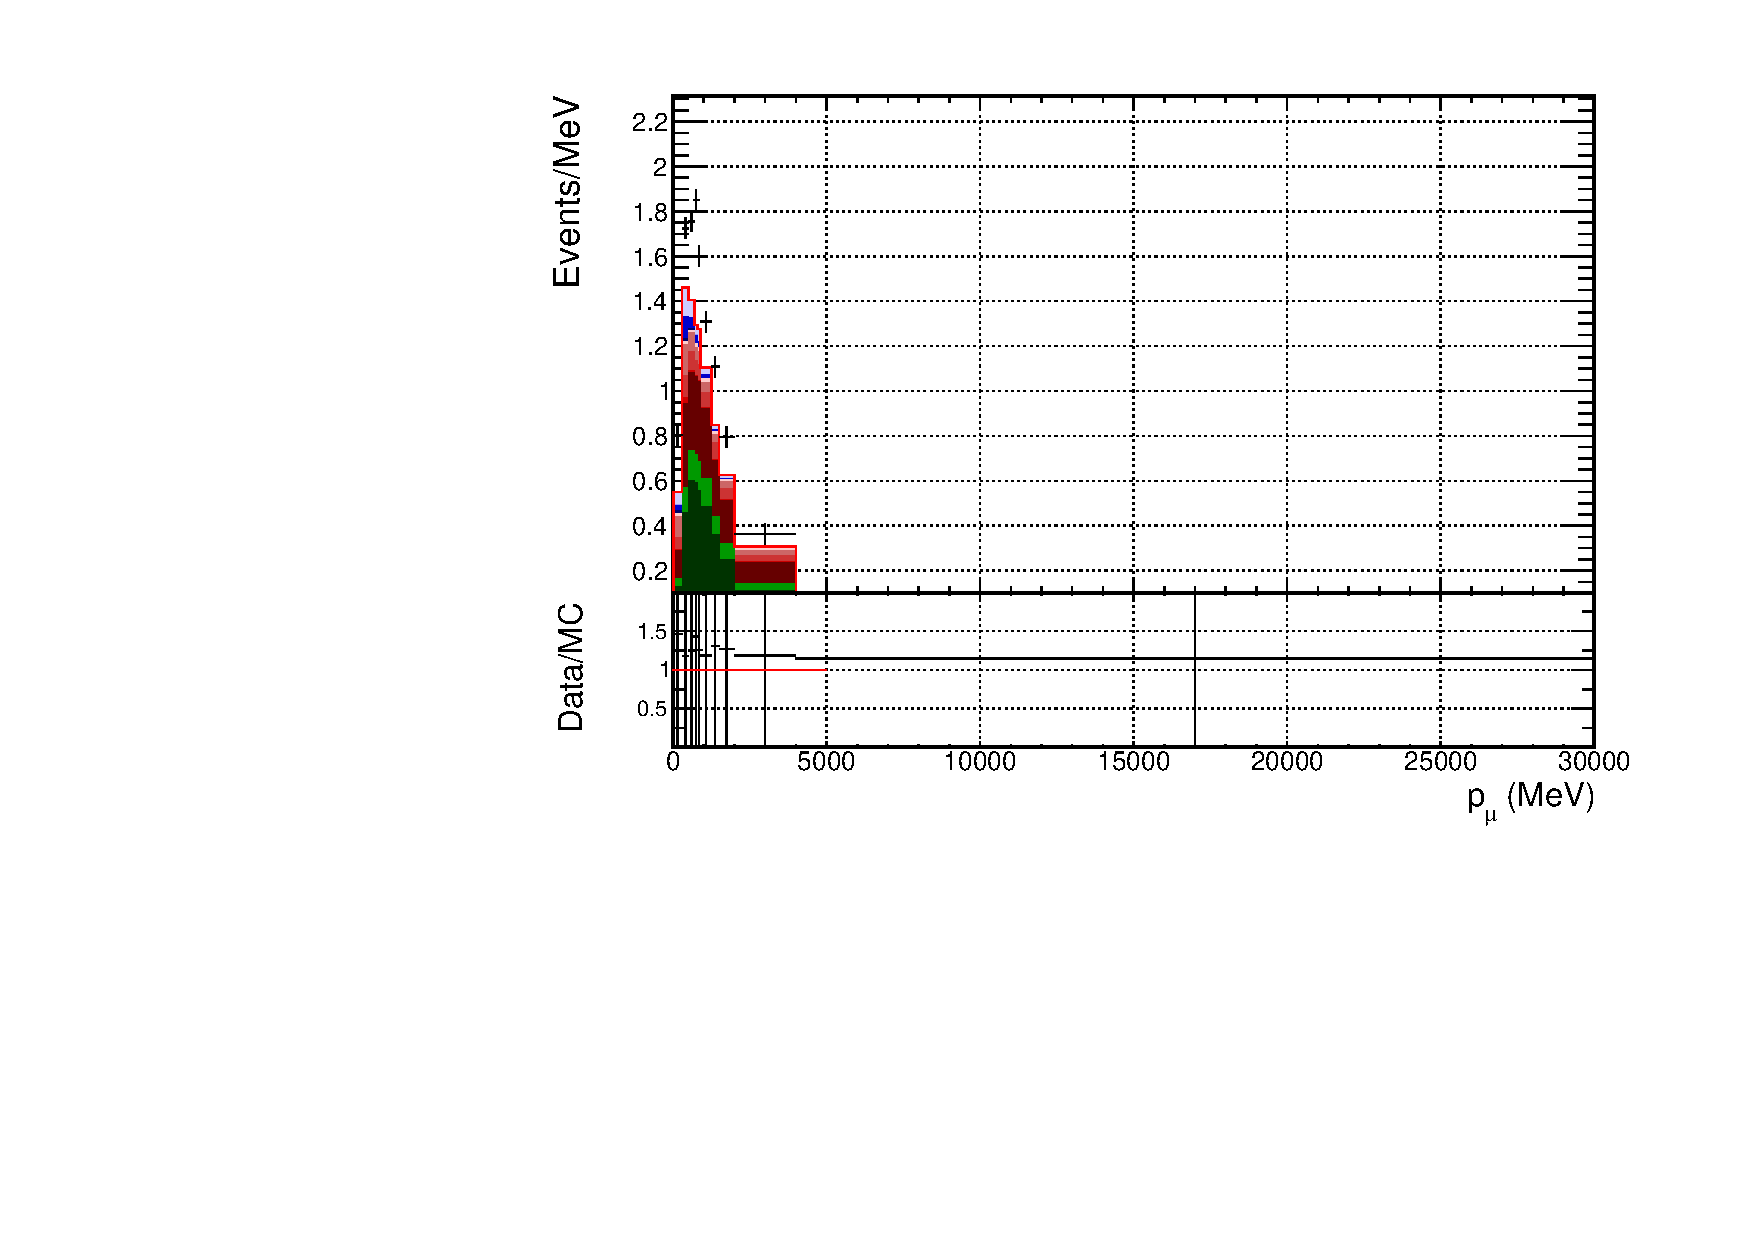
\includegraphics[width=0.95\linewidth]{figs/FGD1_NuMuBkg_CC0pi_in_AntiNu_Mode_p}
  \caption{FGD1 RHC $\nu_{\mu}$ 0$\pi$}
  \label{fig:pstack_FGD1_NuMuBkg_CC0pi_in_AntiNu_Mode}
\end{subfigure}
\begin{subfigure}{.32\textwidth}
  \centering
  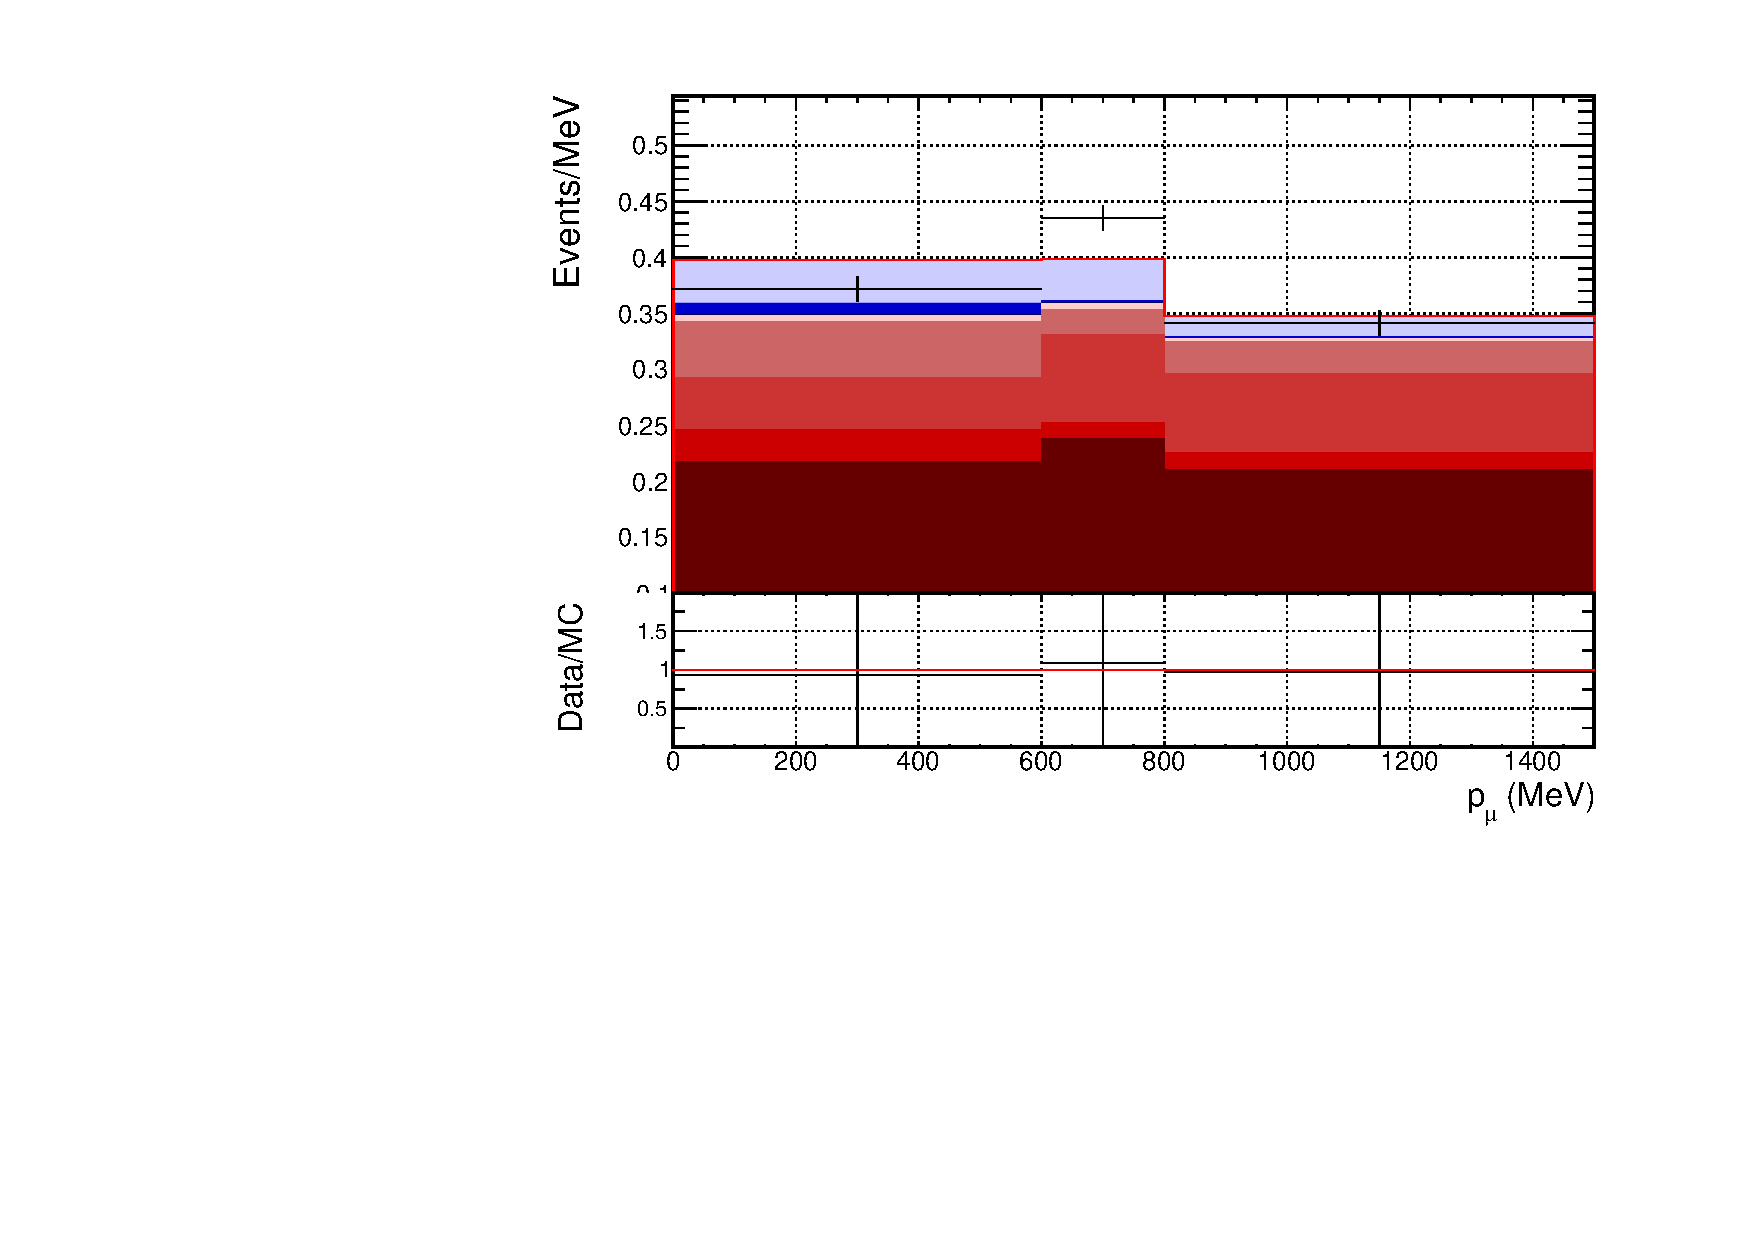
\includegraphics[width=0.95\linewidth]{figs/FGD1_NuMuBkg_CC1pi_in_AntiNu_Mode_p}
  \caption{FGD1 RHC $\nu_{\mu}$ 1$\pi$}
  \label{fig:pstack_FGD1_NuMuBkg_CC1pi_in_AntiNu_Mode}
\end{subfigure}
\begin{subfigure}{.32\textwidth}
  \centering
  \includegraphics[width=0.95\linewidth]{figs/FGD1_NuMuBkg_CCOther_in_AntiNu_Mode_p}
  \caption{FGD1 RHC $\nu_{\mu}$ Other}
  \label{fig:pstack_FGD1_NuMuBkg_CCOther_in_AntiNu_Mode}
\end{subfigure}
\begin{subfigure}{.32\textwidth}
  \centering
  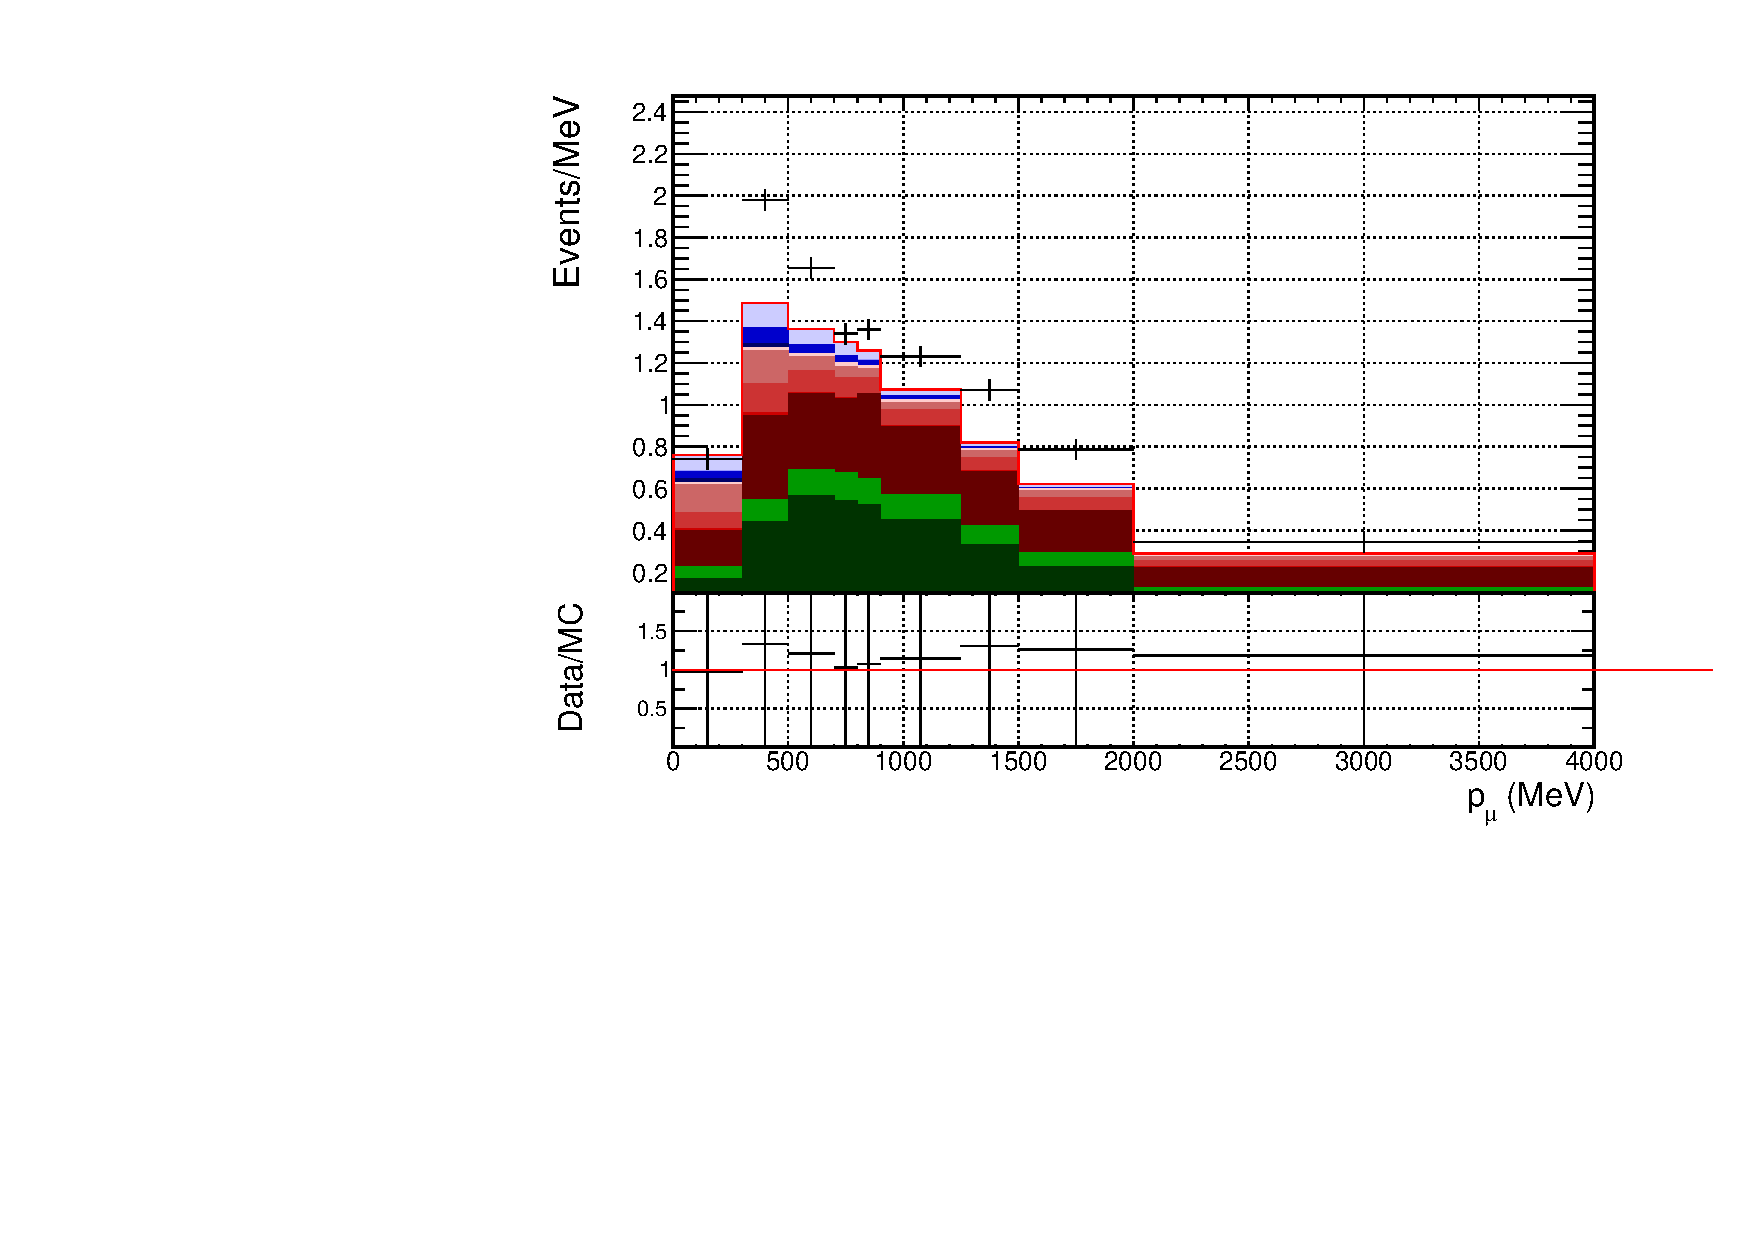
\includegraphics[width=0.95\linewidth]{figs/FGD2_NuMuBkg_CC0pi_in_AntiNu_Mode_p}
  \caption{FGD2 RHC $\nu_{\mu}$ 0$\pi$}
  \label{fig:pstack_FGD2_NuMuBkg_CC0pi_in_AntiNu_Mode}
\end{subfigure}
\begin{subfigure}{.32\textwidth}
  \centering
  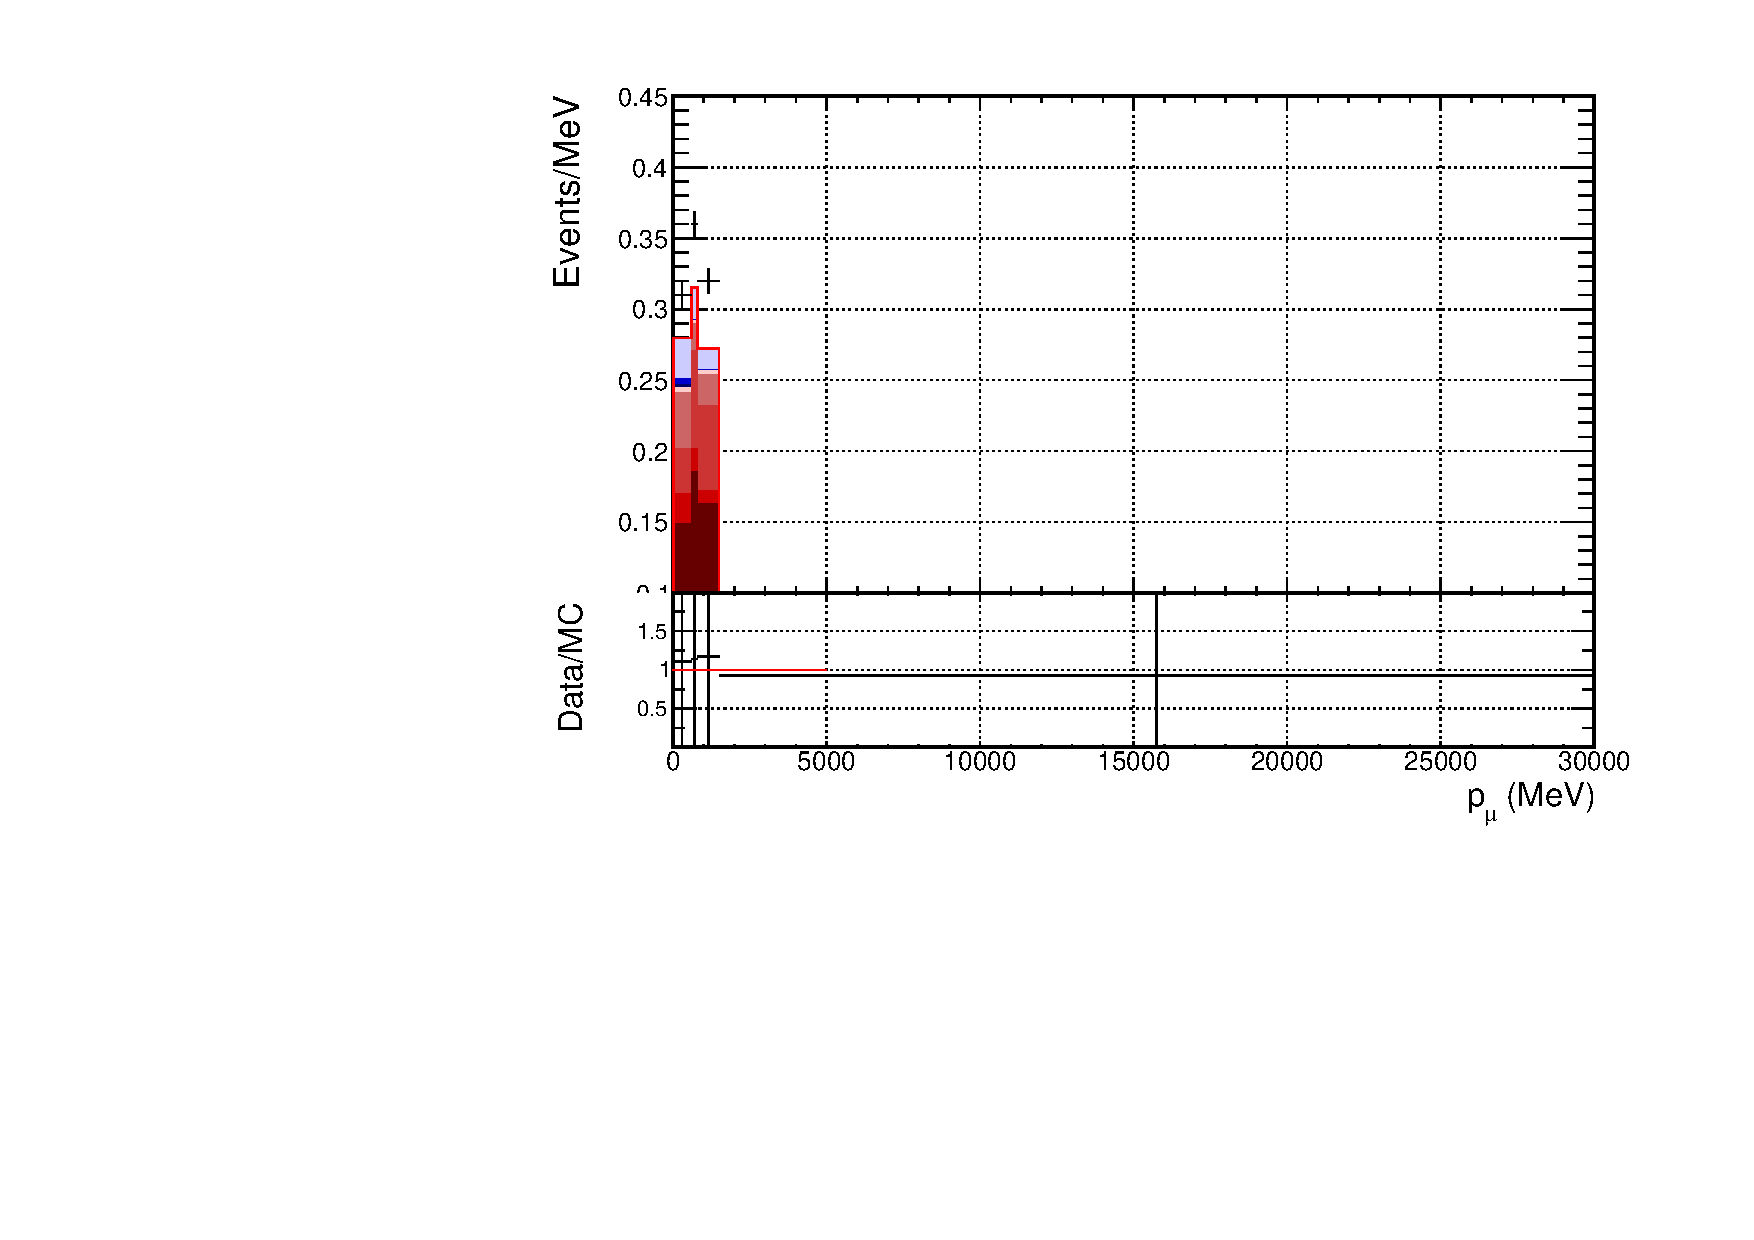
\includegraphics[width=0.95\linewidth]{figs/FGD2_NuMuBkg_CC1pi_in_AntiNu_Mode_p}
  \caption{FGD2 RHC $\nu_{\mu}$ 1$\pi$}
  \label{fig:pstack_FGD2_NuMuBkg_CC1pi_in_AntiNu_Mode}
\end{subfigure}
\begin{subfigure}{.32\textwidth}
  \centering
  \includegraphics[width=0.95\linewidth]{figs/FGD2_NuMuBkg_CCOther_in_AntiNu_Mode_p}
  \caption{FGD2 RHC $\nu_{\mu}$ Other}
  \label{fig:pstack_FGD2_NuMuBkg_CCOther_in_AntiNu_Mode}
\end{subfigure}
\caption{P$_{\mu}$ projections of data and nominal MC broken down by interaction mode.}
\label{fig:pstack}
\end{figure}

The projections onto the $cos\theta_{\mu}$ axis are shown in Figure \ref{fig:tstack}, along with the data and interaction mode breakdown.

The CC 0$\pi$ and CC Other samples again show oscillatory behaviour in the ratio of data to MC. At high angle, the ratio increases and decreases, but always remains $>1$. For the CC 1$\pi$ samples,  the ratio is again more flat, but at high angle oscillates between the MC over and underestimating the data. This is again consistent across the FGDs.

\begin{figure}
\centering
\begin{subfigure}{.35\textwidth}
  \centering
  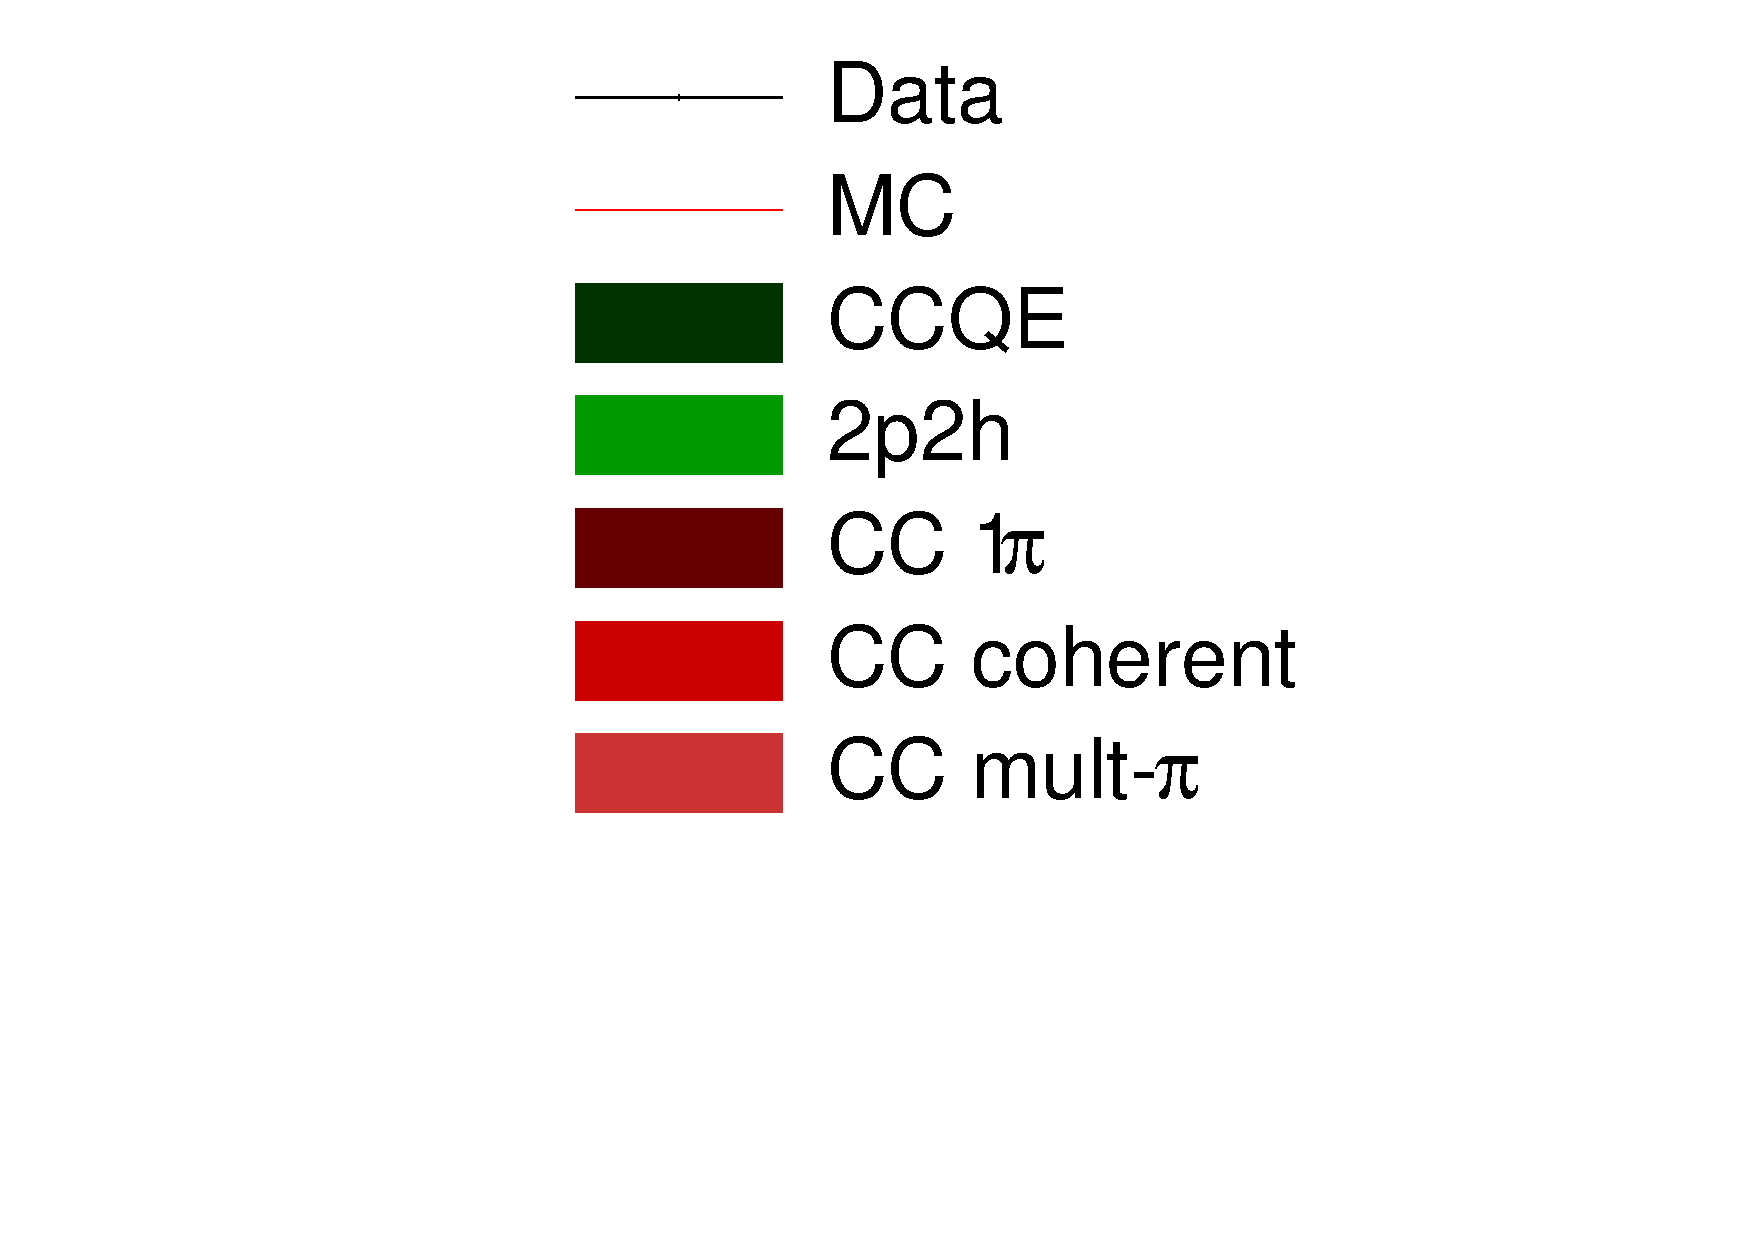
\includegraphics[width=0.7\linewidth]{figs/legend}
\end{subfigure}
\begin{subfigure}{.35\textwidth}
  \centering
  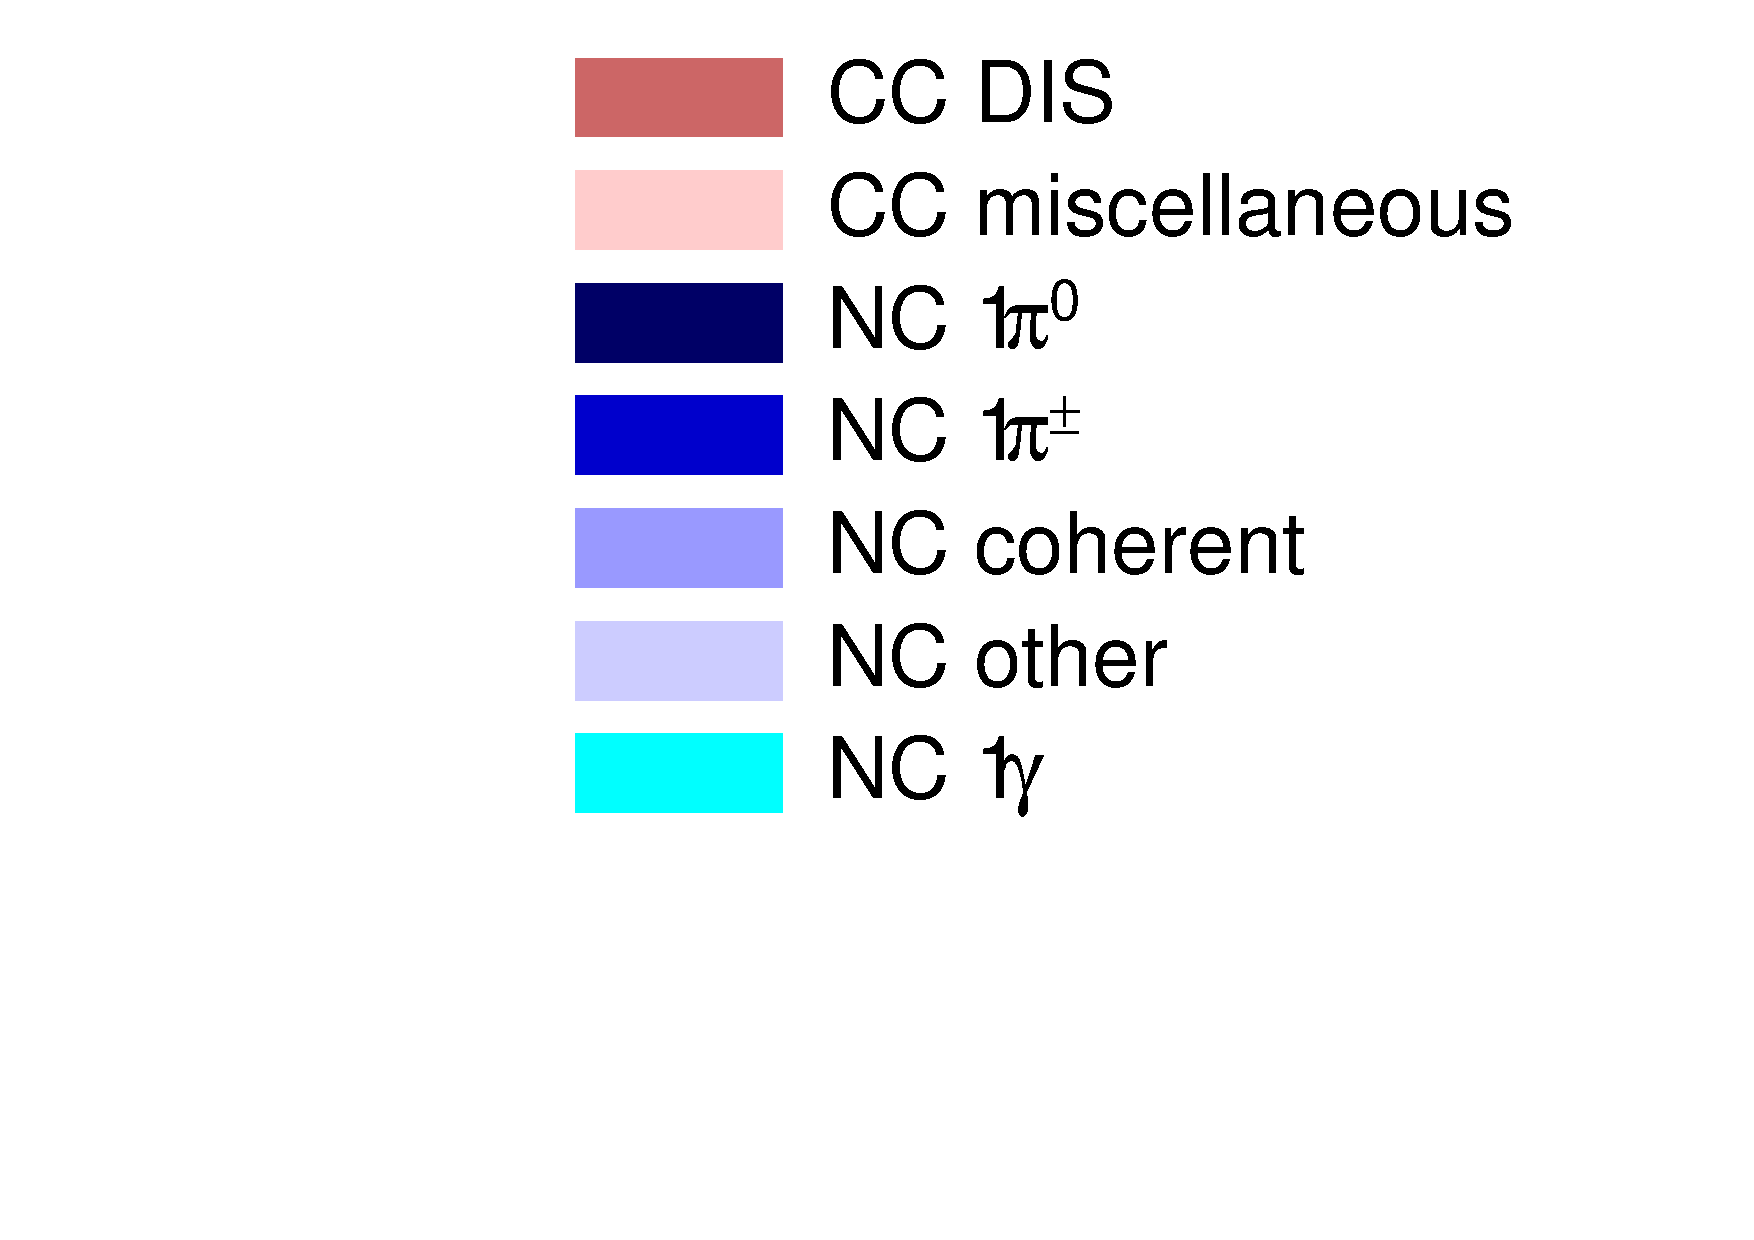
\includegraphics[width=0.7\linewidth]{figs/legend2}
\end{subfigure}
\begin{subfigure}{.32\textwidth}
  \centering
  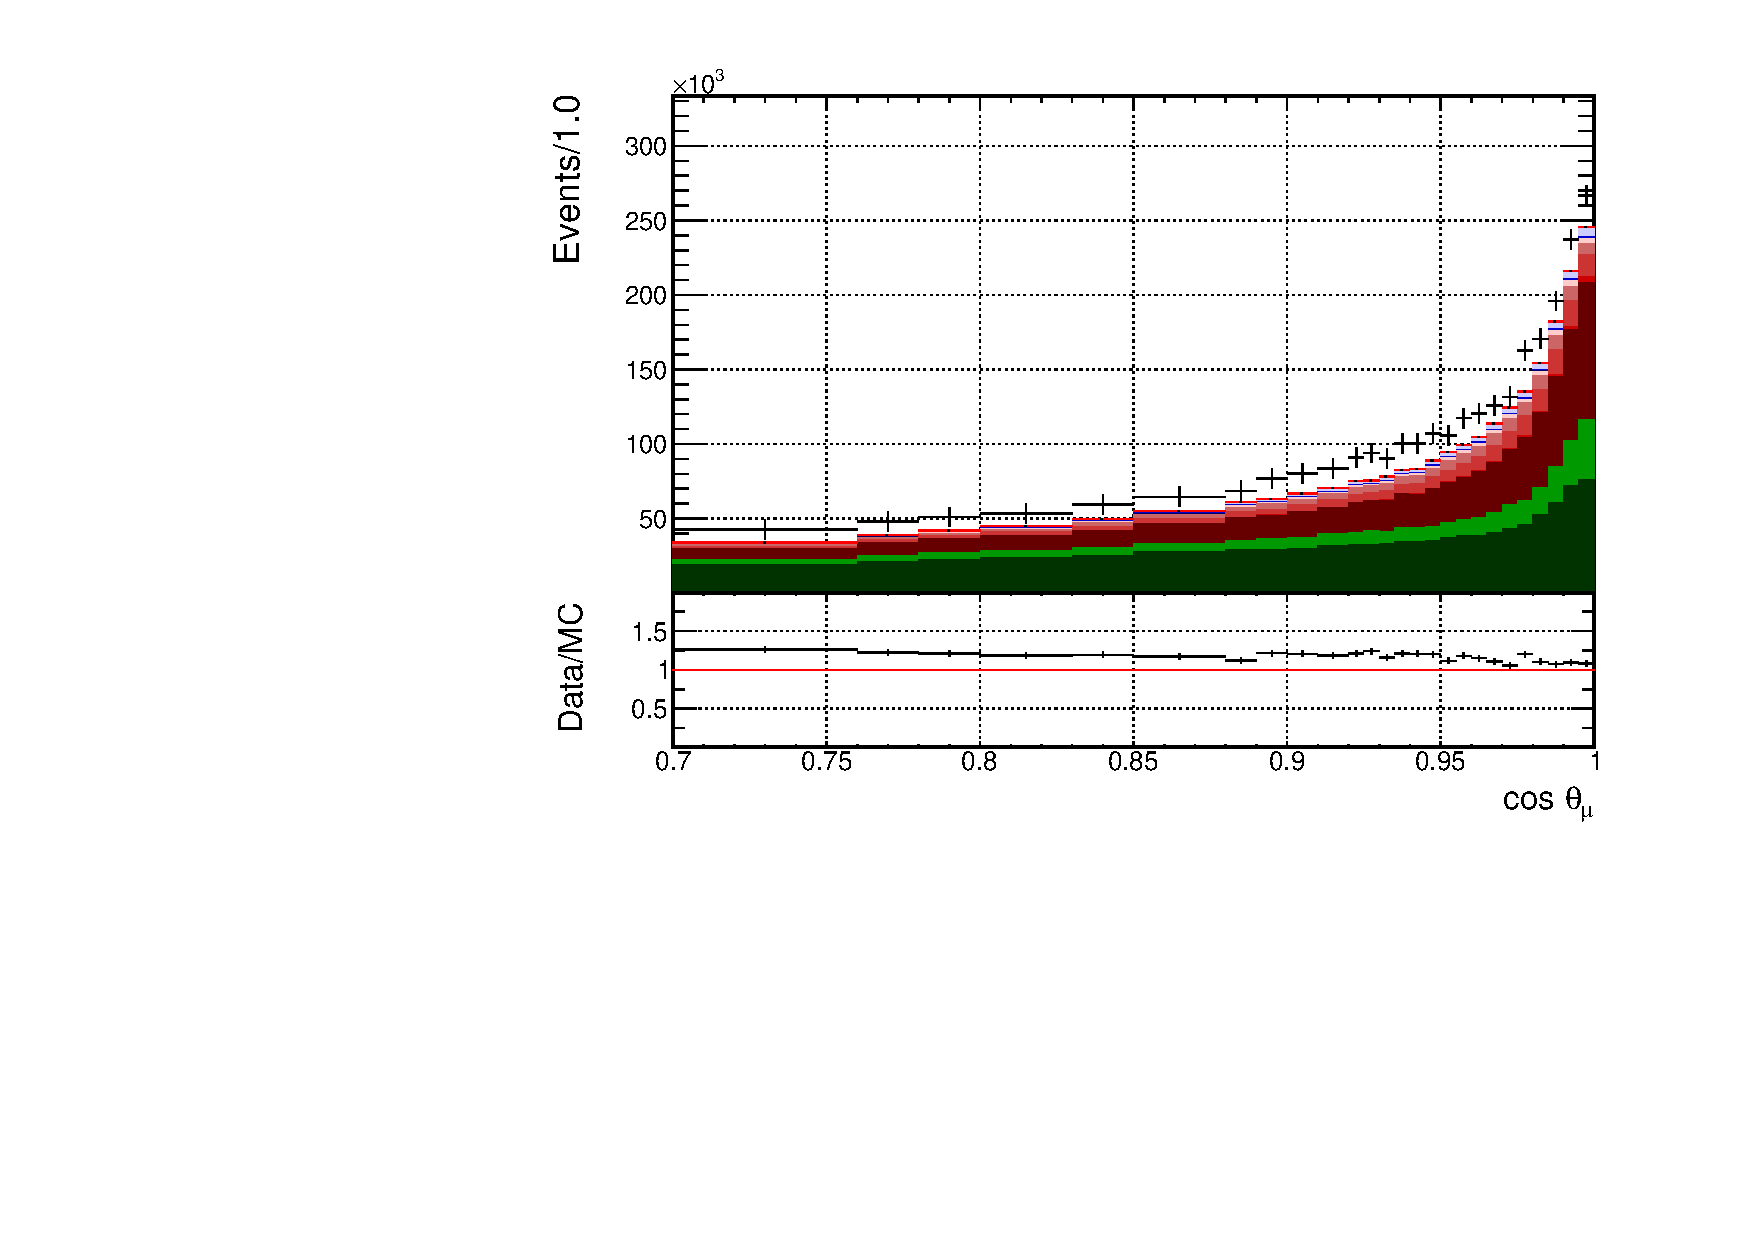
\includegraphics[width=0.95\linewidth]{figs/FGD2_numuCC_0pi_t}
  \caption{FGD1 FHC $\nu_{\mu}$ 0$\pi$}
  \label{fig:tstack_FGD1_numuCC_0pi}
\end{subfigure}
\begin{subfigure}{.32\textwidth}
  \centering
  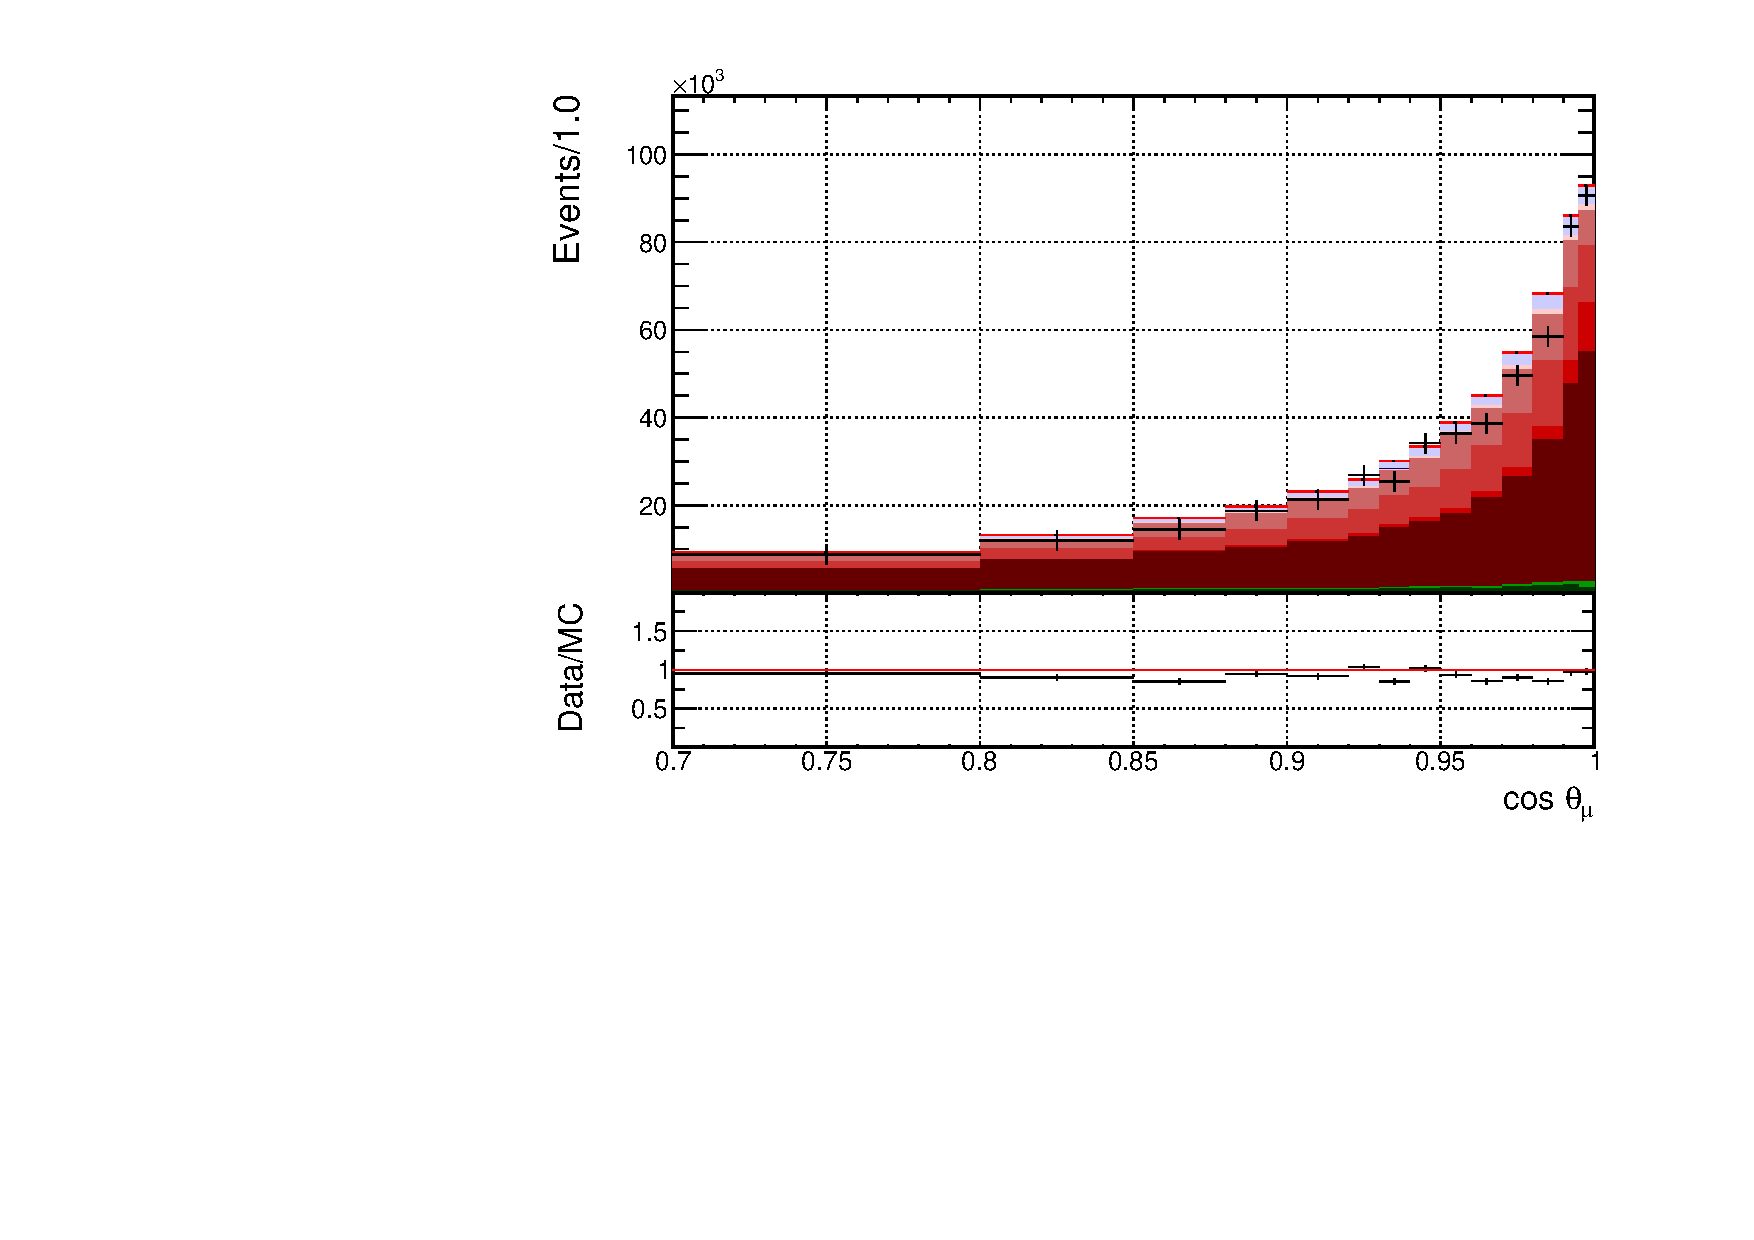
\includegraphics[width=0.95\linewidth]{figs/FGD1_numuCC_1pi_t}
  \caption{FGD1 FHC $\nu_{\mu}$ 1$\pi$}
  \label{fig:tstack_FGD1_numuCC_1pi}
\end{subfigure}
\begin{subfigure}{.32\textwidth}
  \centering
  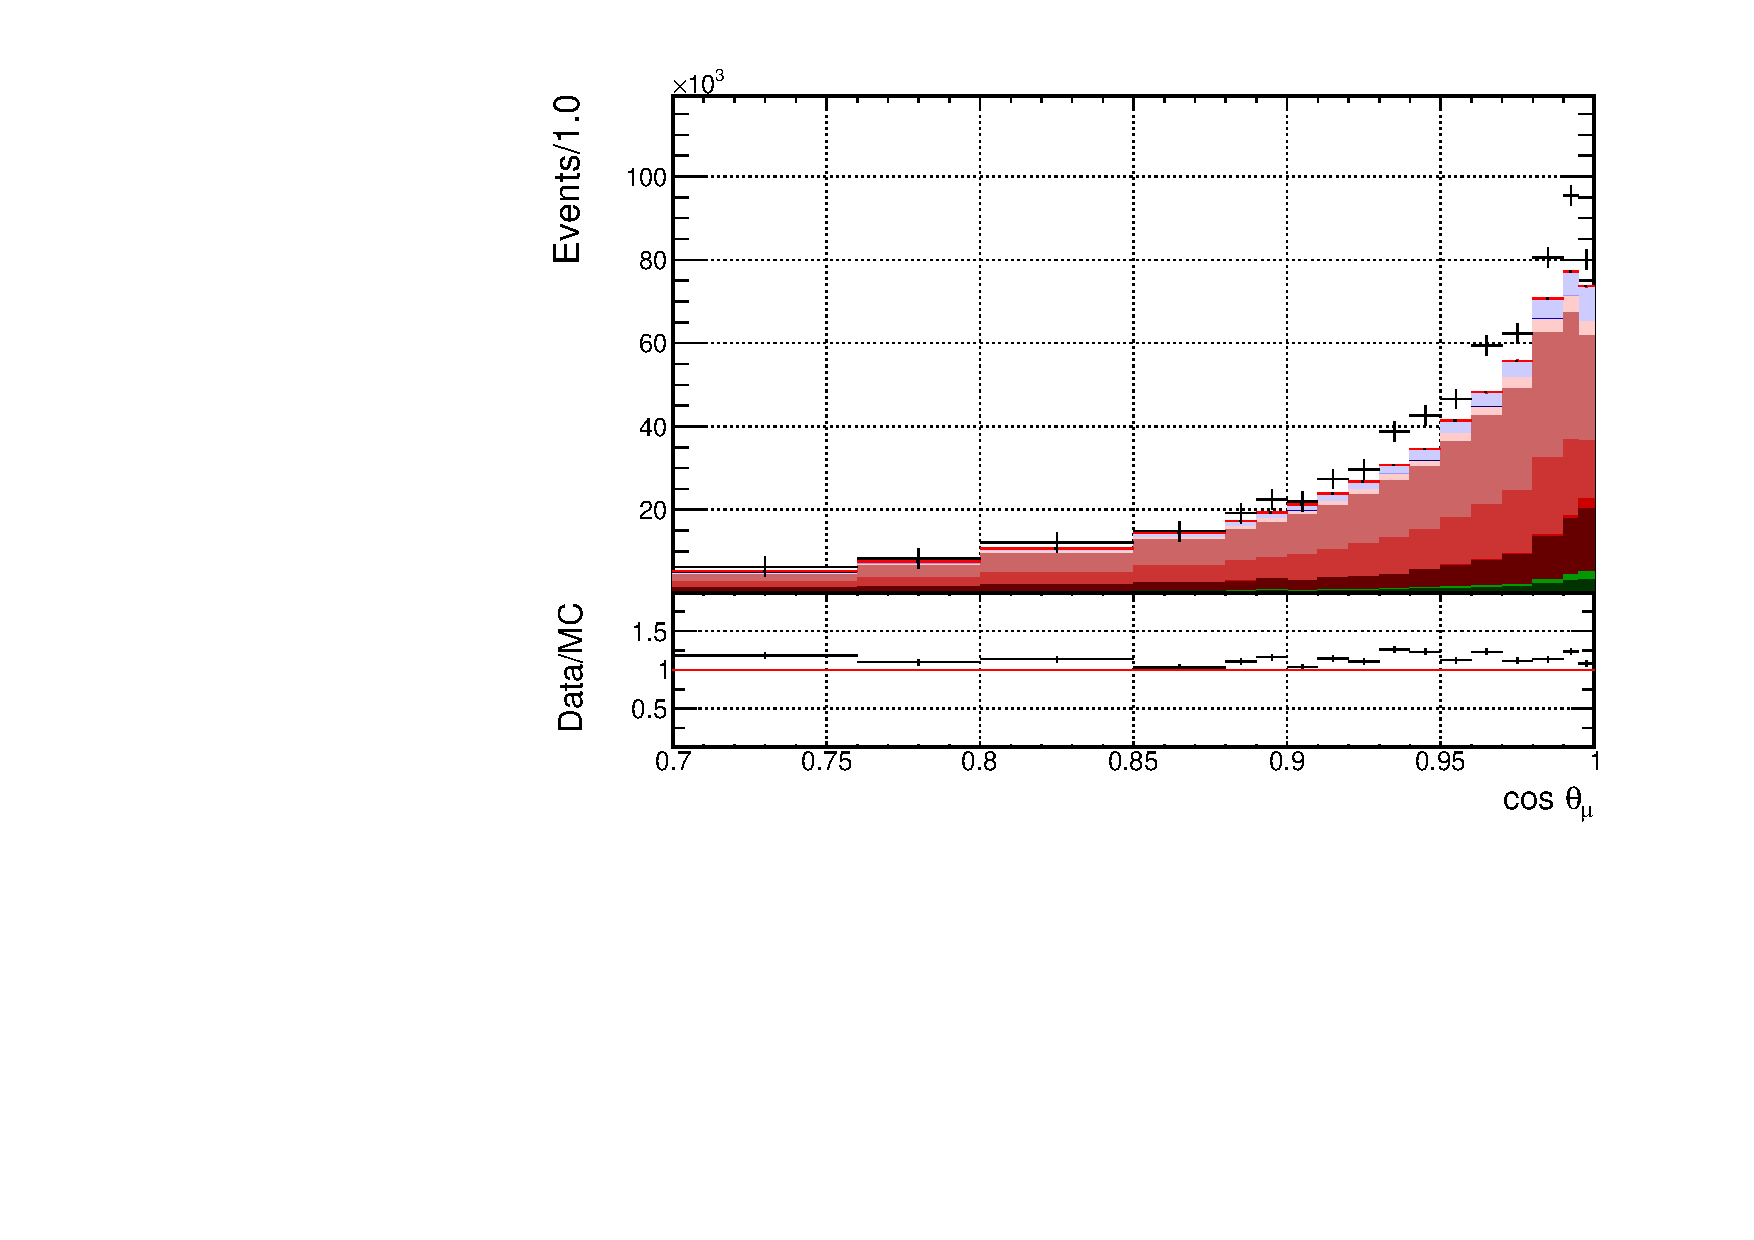
\includegraphics[width=0.95\linewidth]{figs/FGD1_numuCC_other_t}
  \caption{FGD1 FHC $\nu_{\mu}$ Other}
  \label{fig:tstack_FGD1_numuCC_other}
\end{subfigure}
\centering
\begin{subfigure}{.32\textwidth}
  \centering
  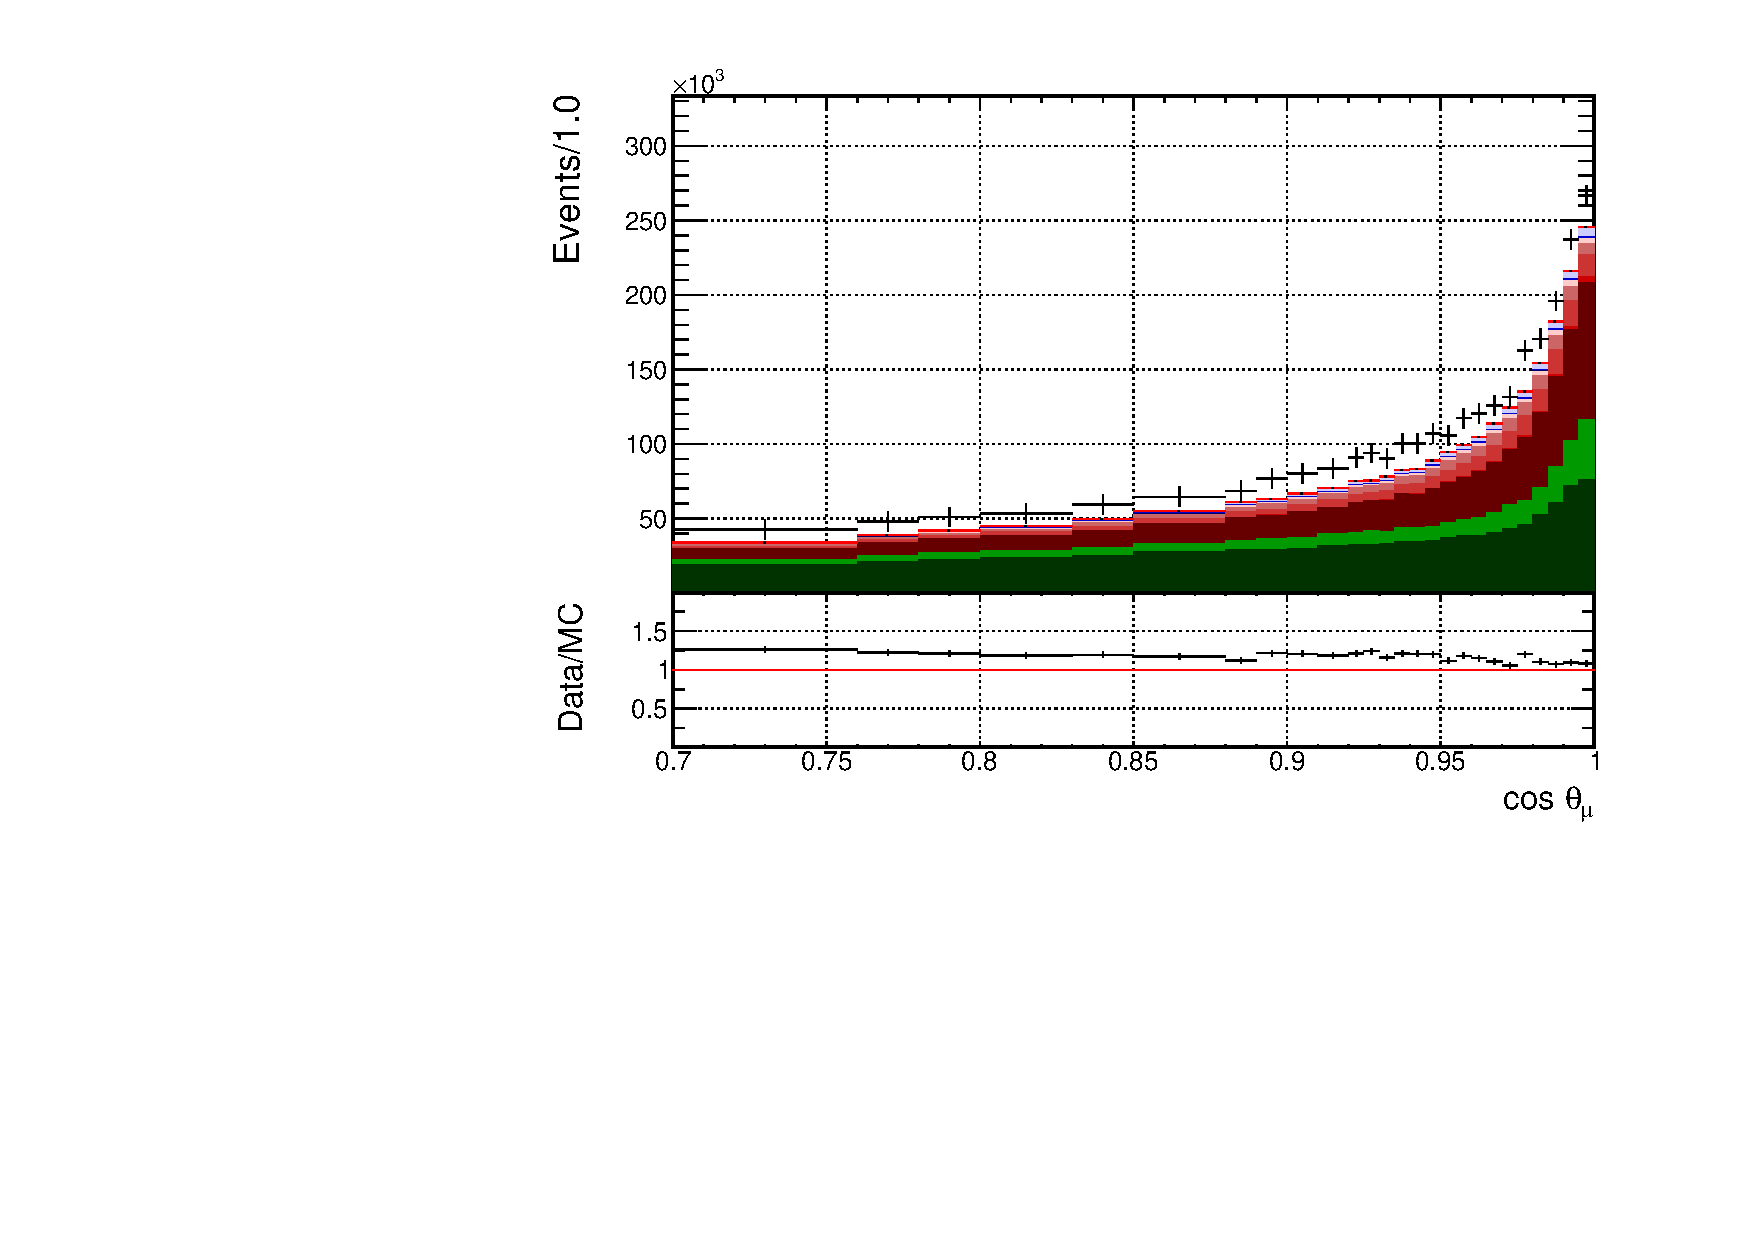
\includegraphics[width=0.95\linewidth]{figs/FGD2_numuCC_0pi_t}
  \caption{FGD2 FHC $\nu_{\mu}$ 0$\pi$}
  \label{fig:tstack_FGD2_numuCC_0pi}
\end{subfigure}
\begin{subfigure}{.32\textwidth}
  \centering
  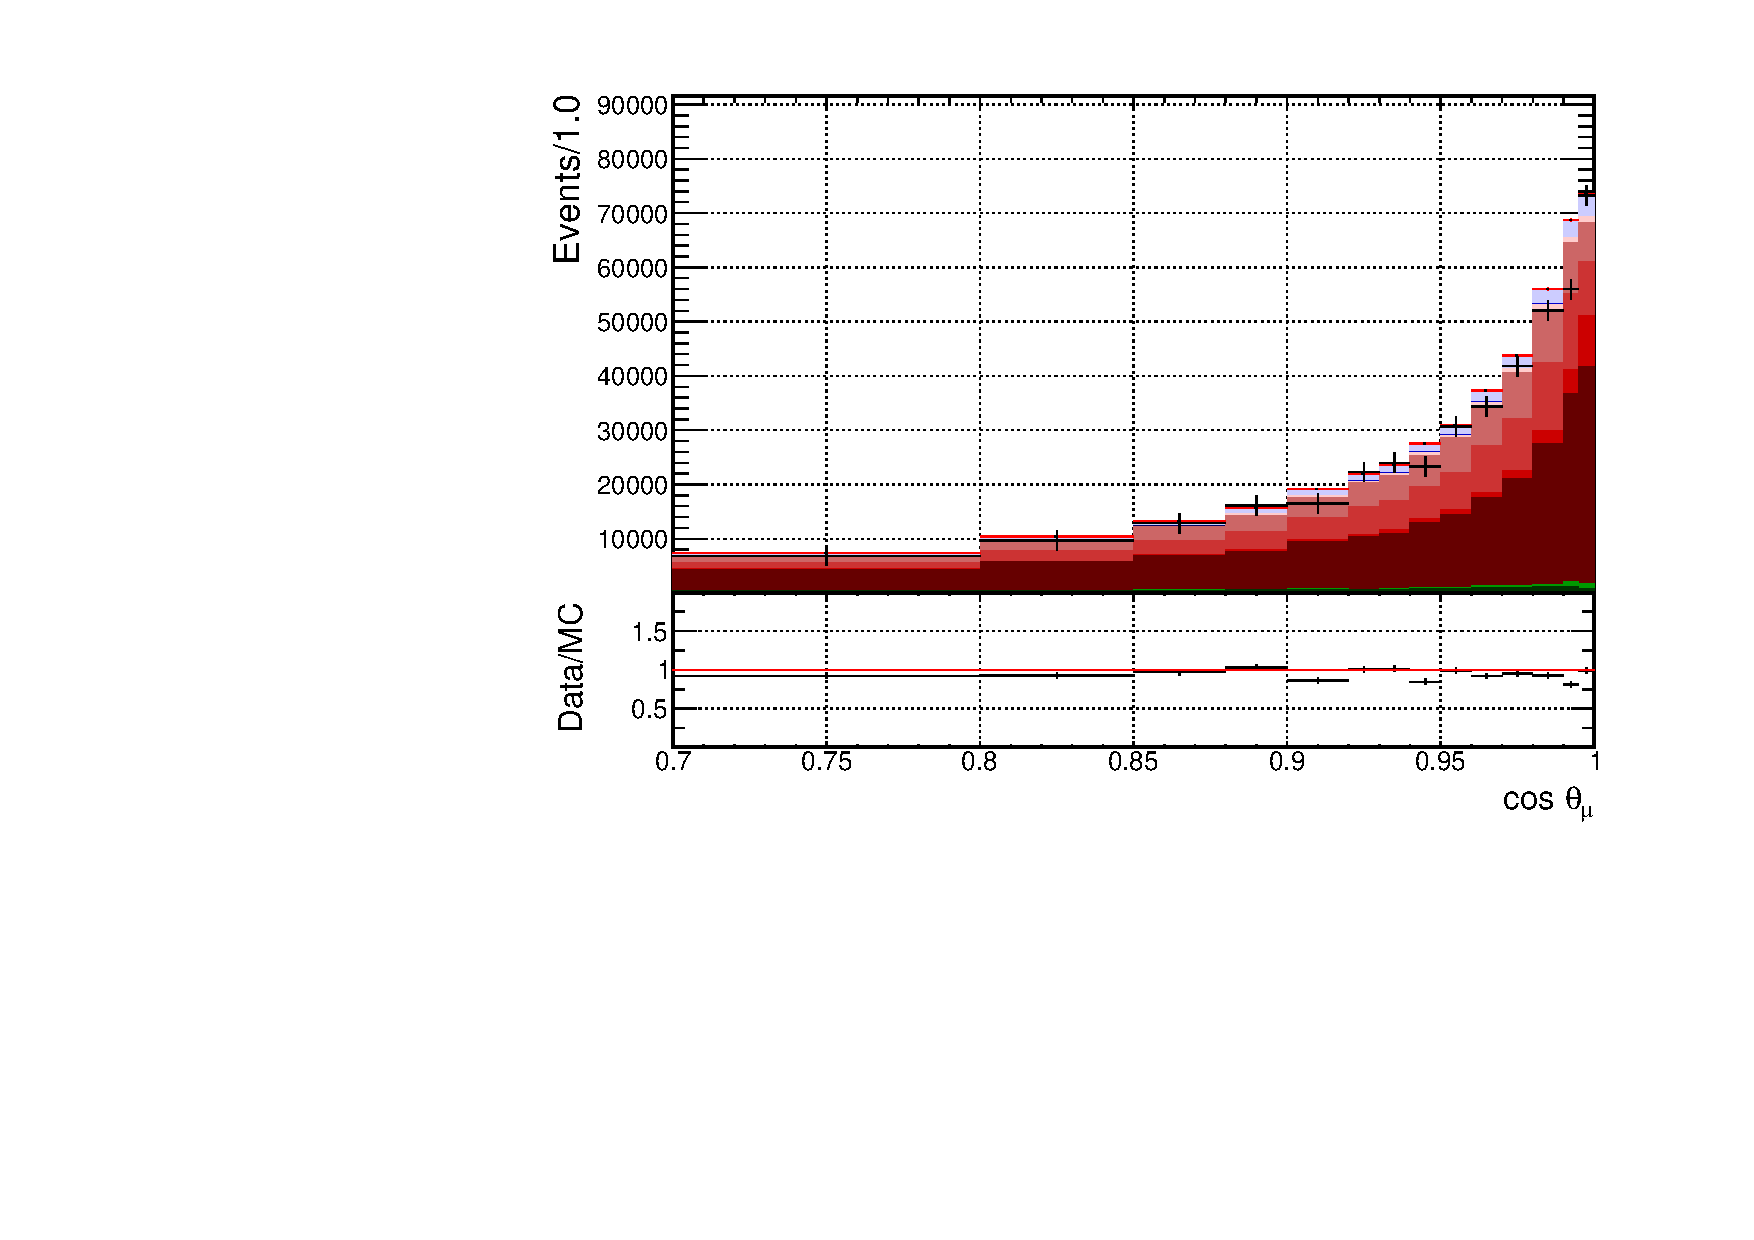
\includegraphics[width=0.95\linewidth]{figs/FGD2_numuCC_1pi_t}
  \caption{FGD2 FHC $\nu_{\mu}$ 1$\pi$}
  \label{fig:tstack_FGD2_numuCC_1pi}
\end{subfigure}
\begin{subfigure}{.32\textwidth}
  \centering
  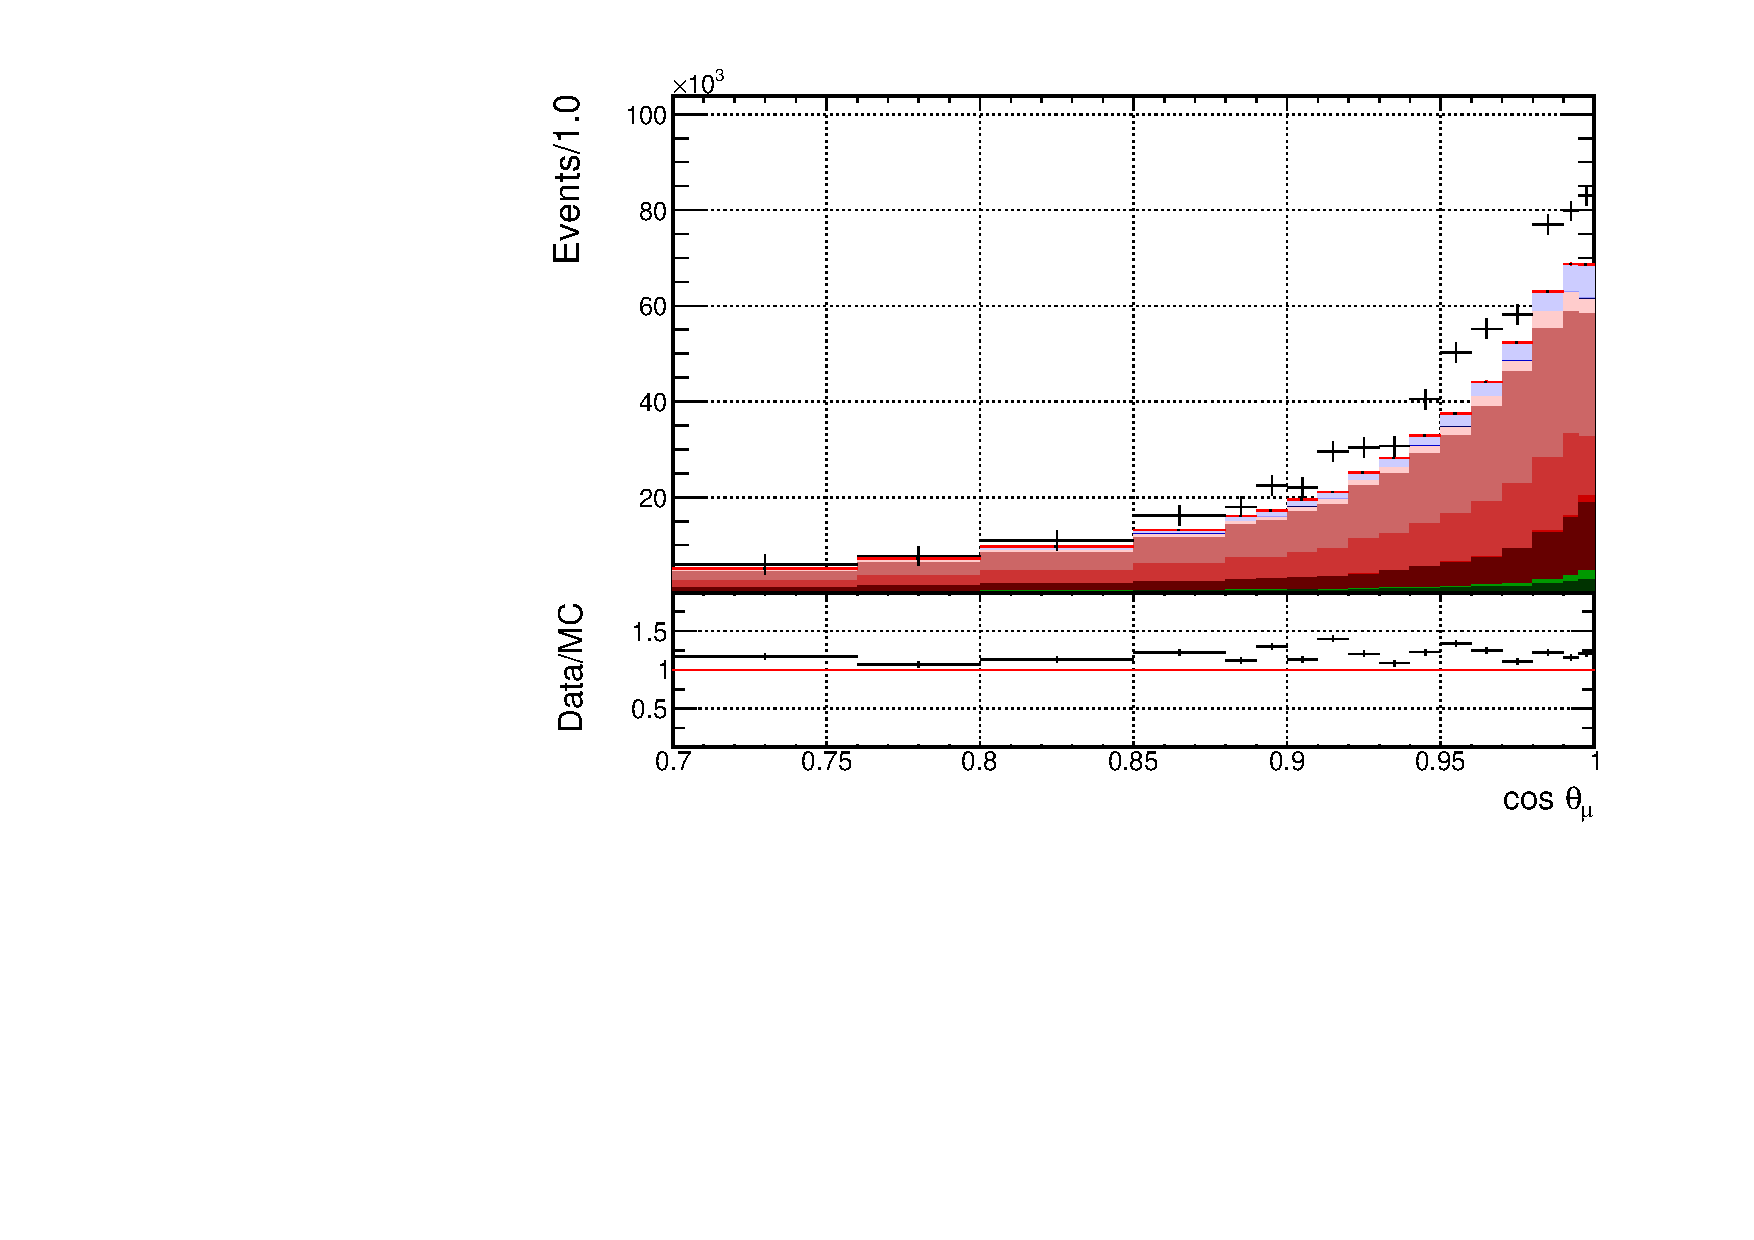
\includegraphics[width=0.95\linewidth]{figs/FGD2_numuCC_other_t}
  \caption{FGD2 $\nu_{\mu}$ Other}
  \label{fig:tstack_FGD2_numuCC_other}
\end{subfigure}
\centering
\begin{subfigure}{.32\textwidth}
  \centering
  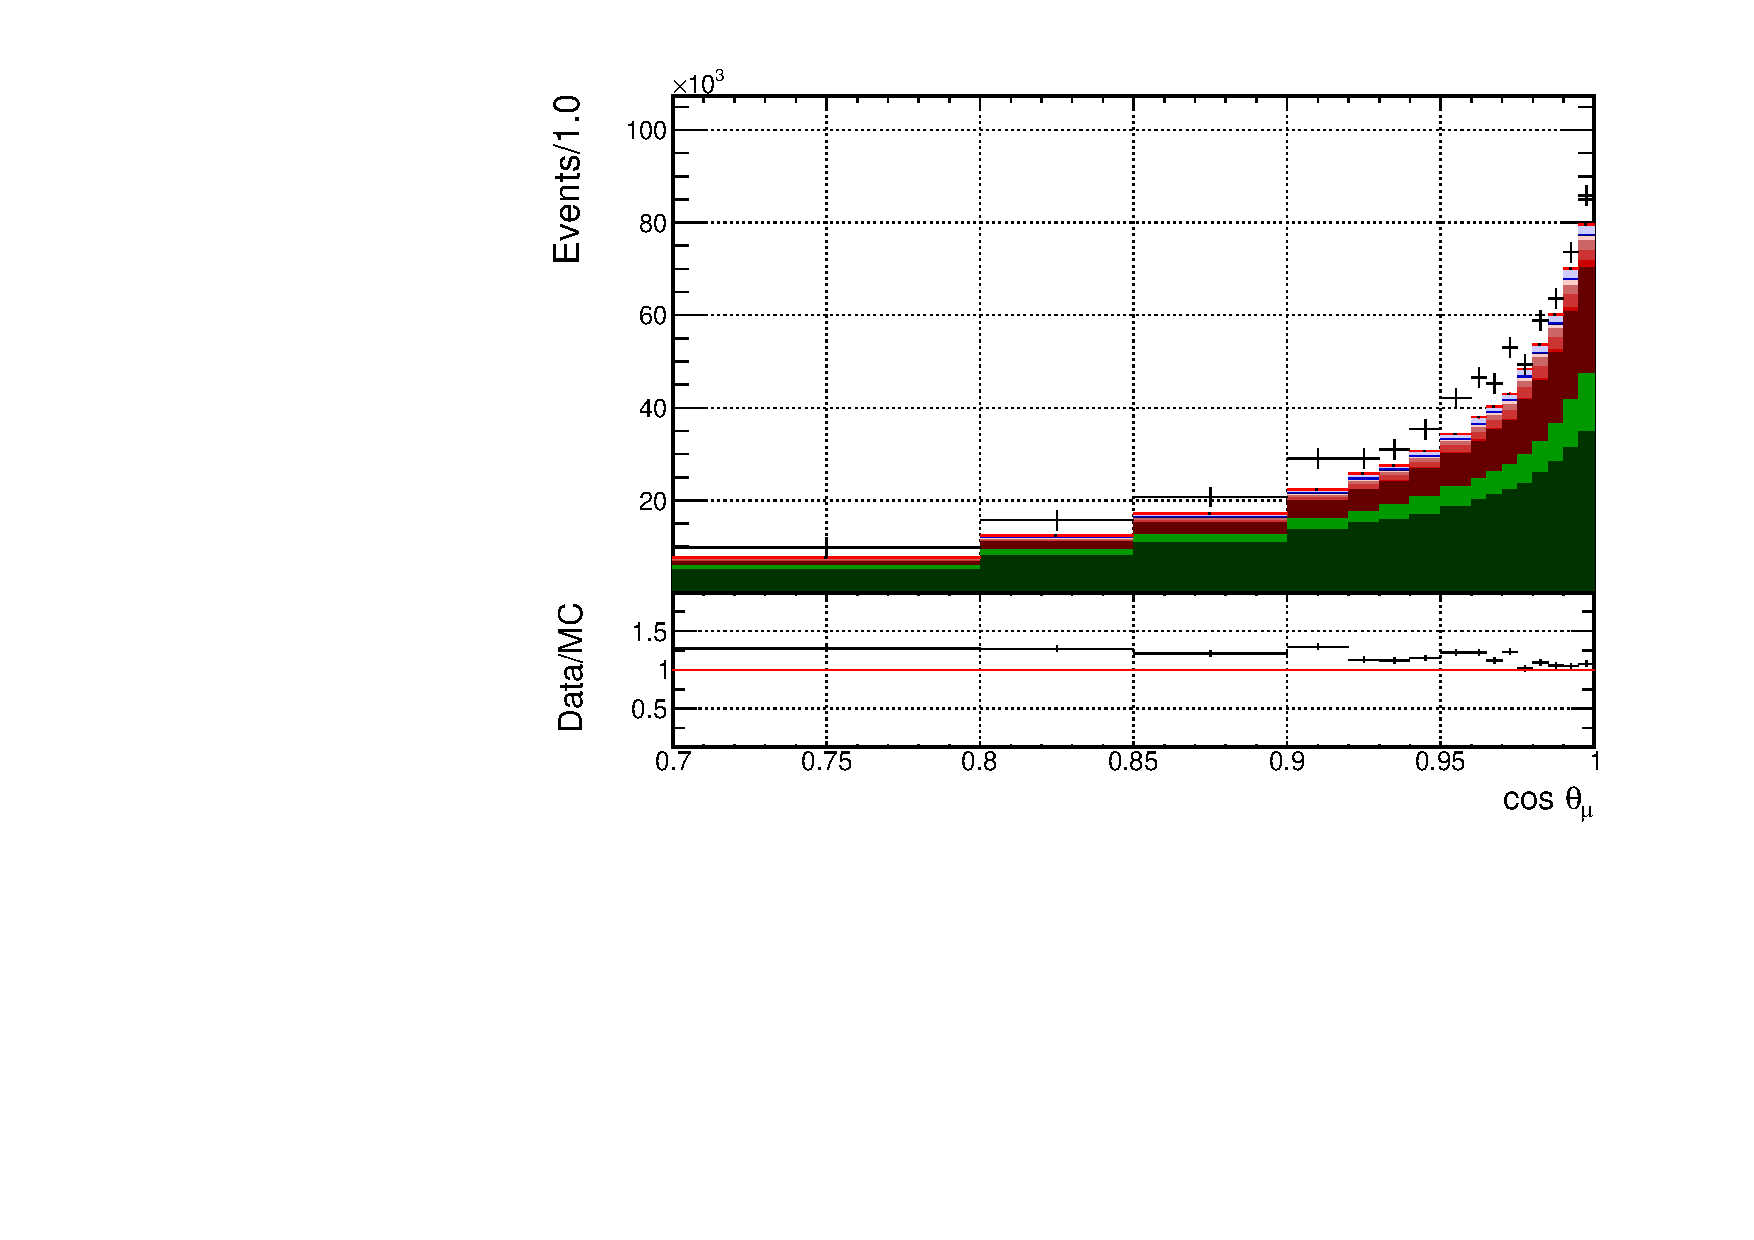
\includegraphics[width=0.95\linewidth]{figs/FGD1_anti-numuCC_0pi_t}
  \caption{FGD1 RHC $\bar{\nu_{\mu}}$ 0$\pi$}
  \label{fig:tstack_FGD1_anti-numuCC_0pi}
\end{subfigure}
\begin{subfigure}{.32\textwidth}
  \centering
  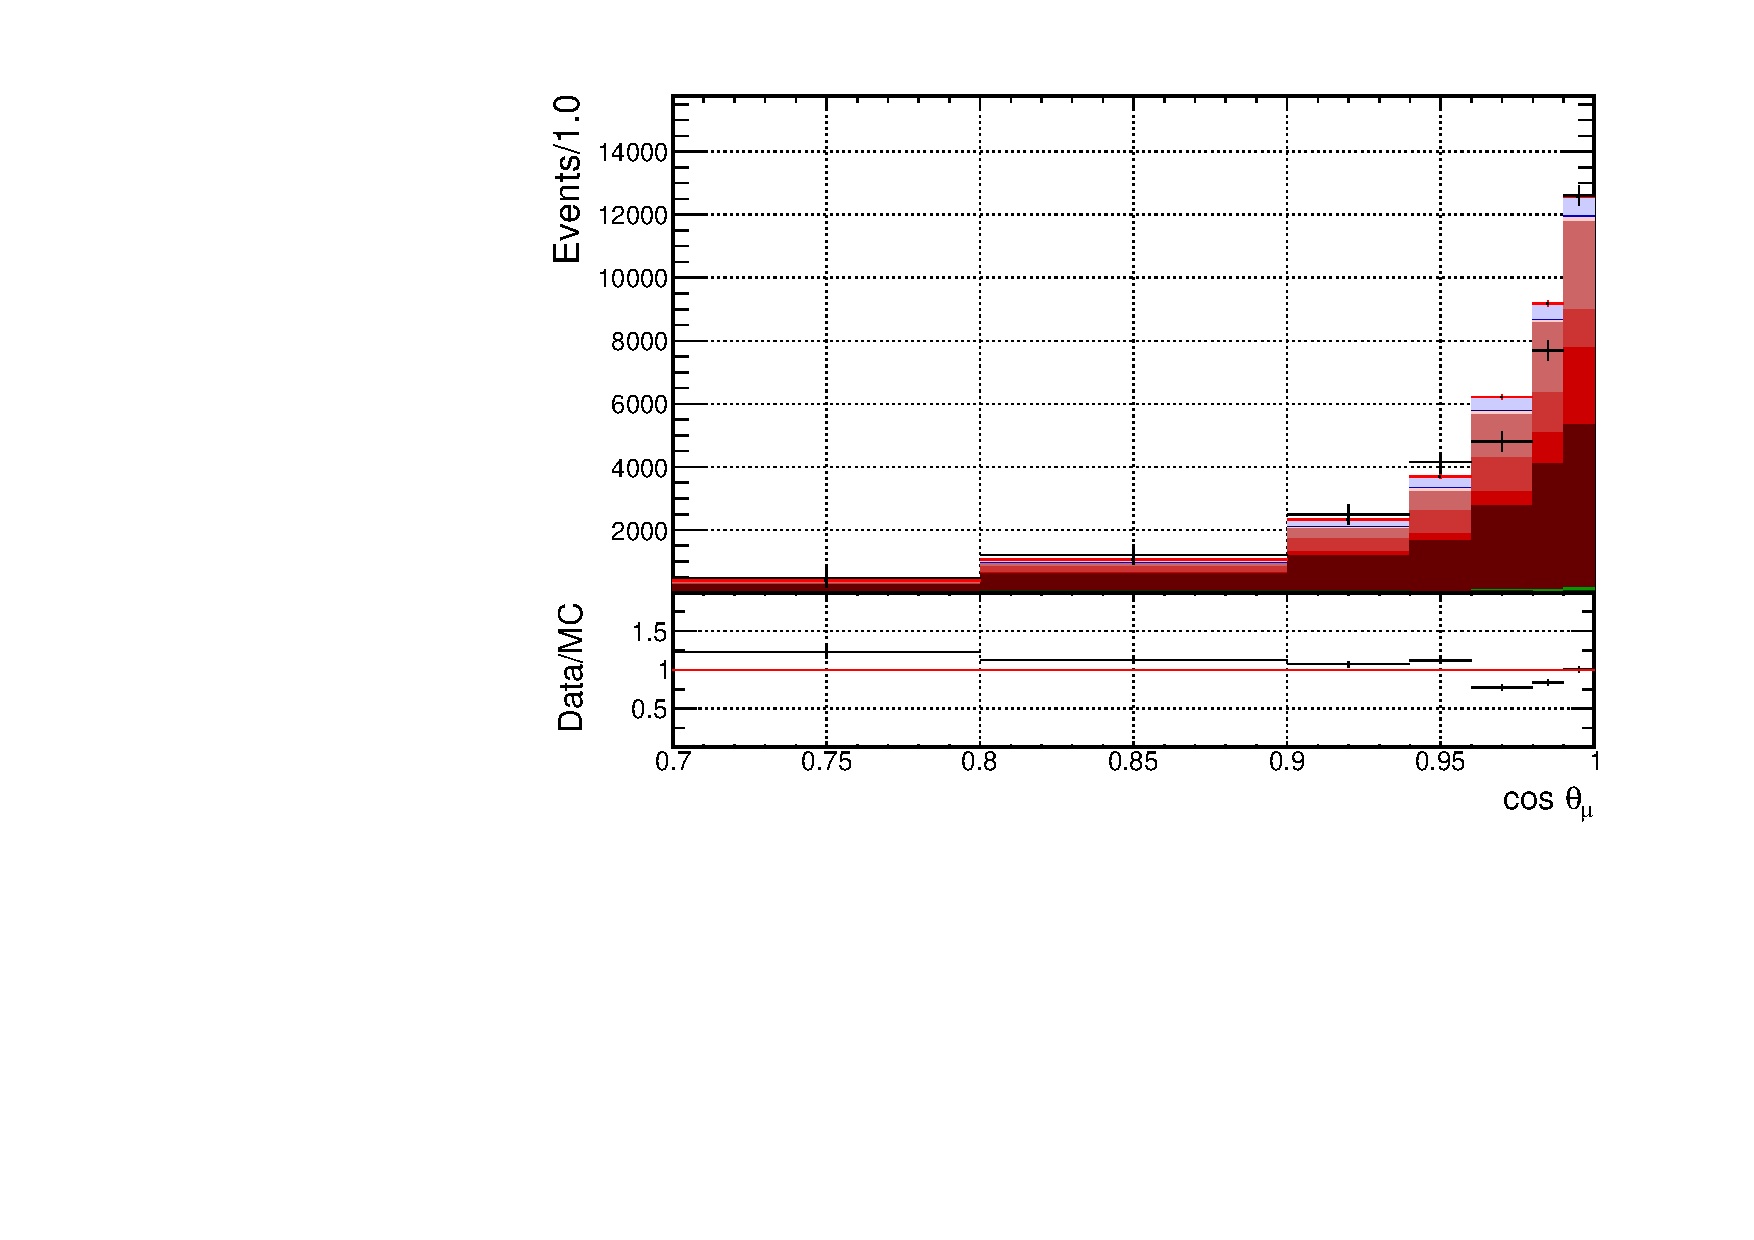
\includegraphics[width=0.95\linewidth]{figs/FGD1_anti-numuCC_1pi_t}
  \caption{FGD1 RHC $\bar{\nu_{\mu}}$ 1$\pi$}
  \label{fig:tstack_tstack_FGD1_anti-numuCC_1pi}
\end{subfigure}
\begin{subfigure}{.32\textwidth}
  \centering
  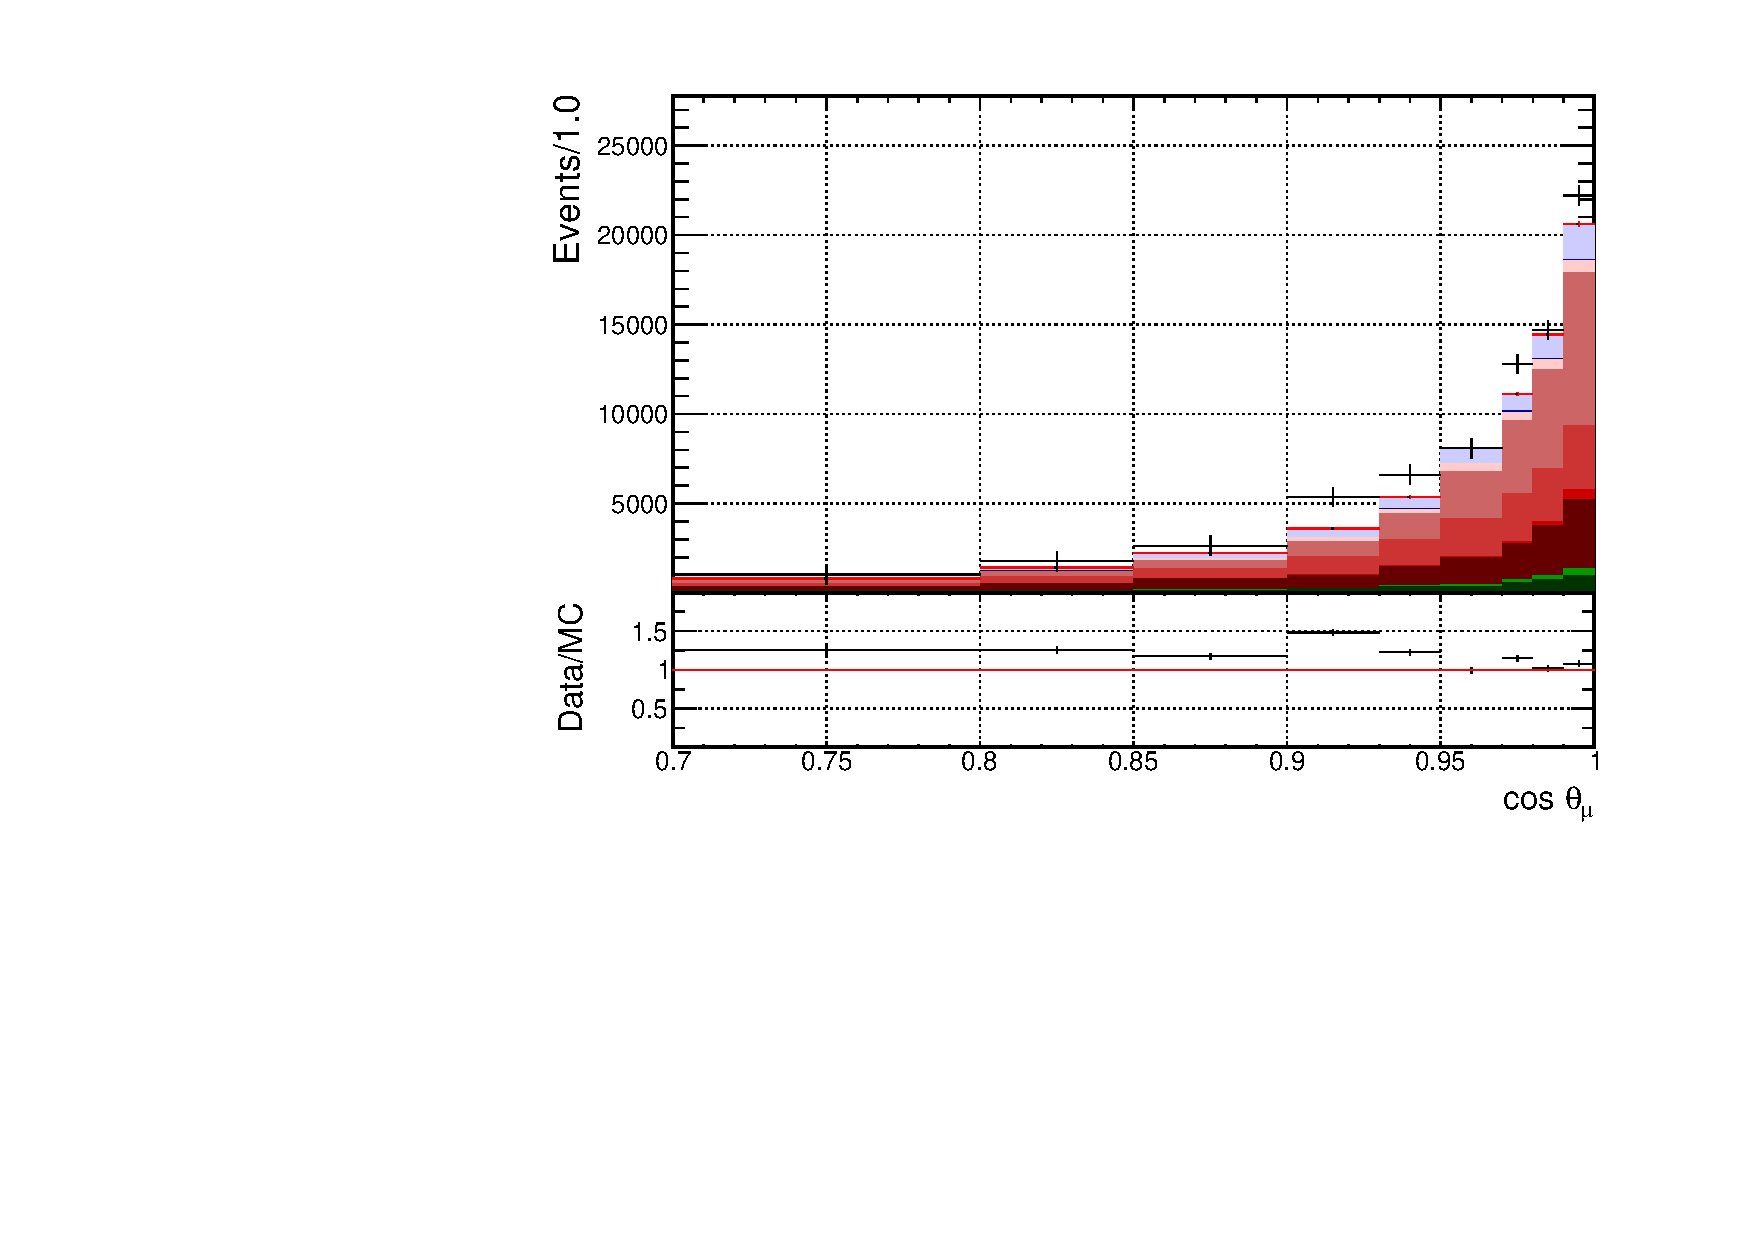
\includegraphics[width=0.95\linewidth]{figs/FGD1_anti-numuCC_other_t}
  \caption{FGD1 RHC $\bar{\nu_{\mu}}$ Other}
  \label{fig:tstack_FGD1_anti-numuCC_other}
\end{subfigure}
\centering
\begin{subfigure}{.32\textwidth}
  \centering
  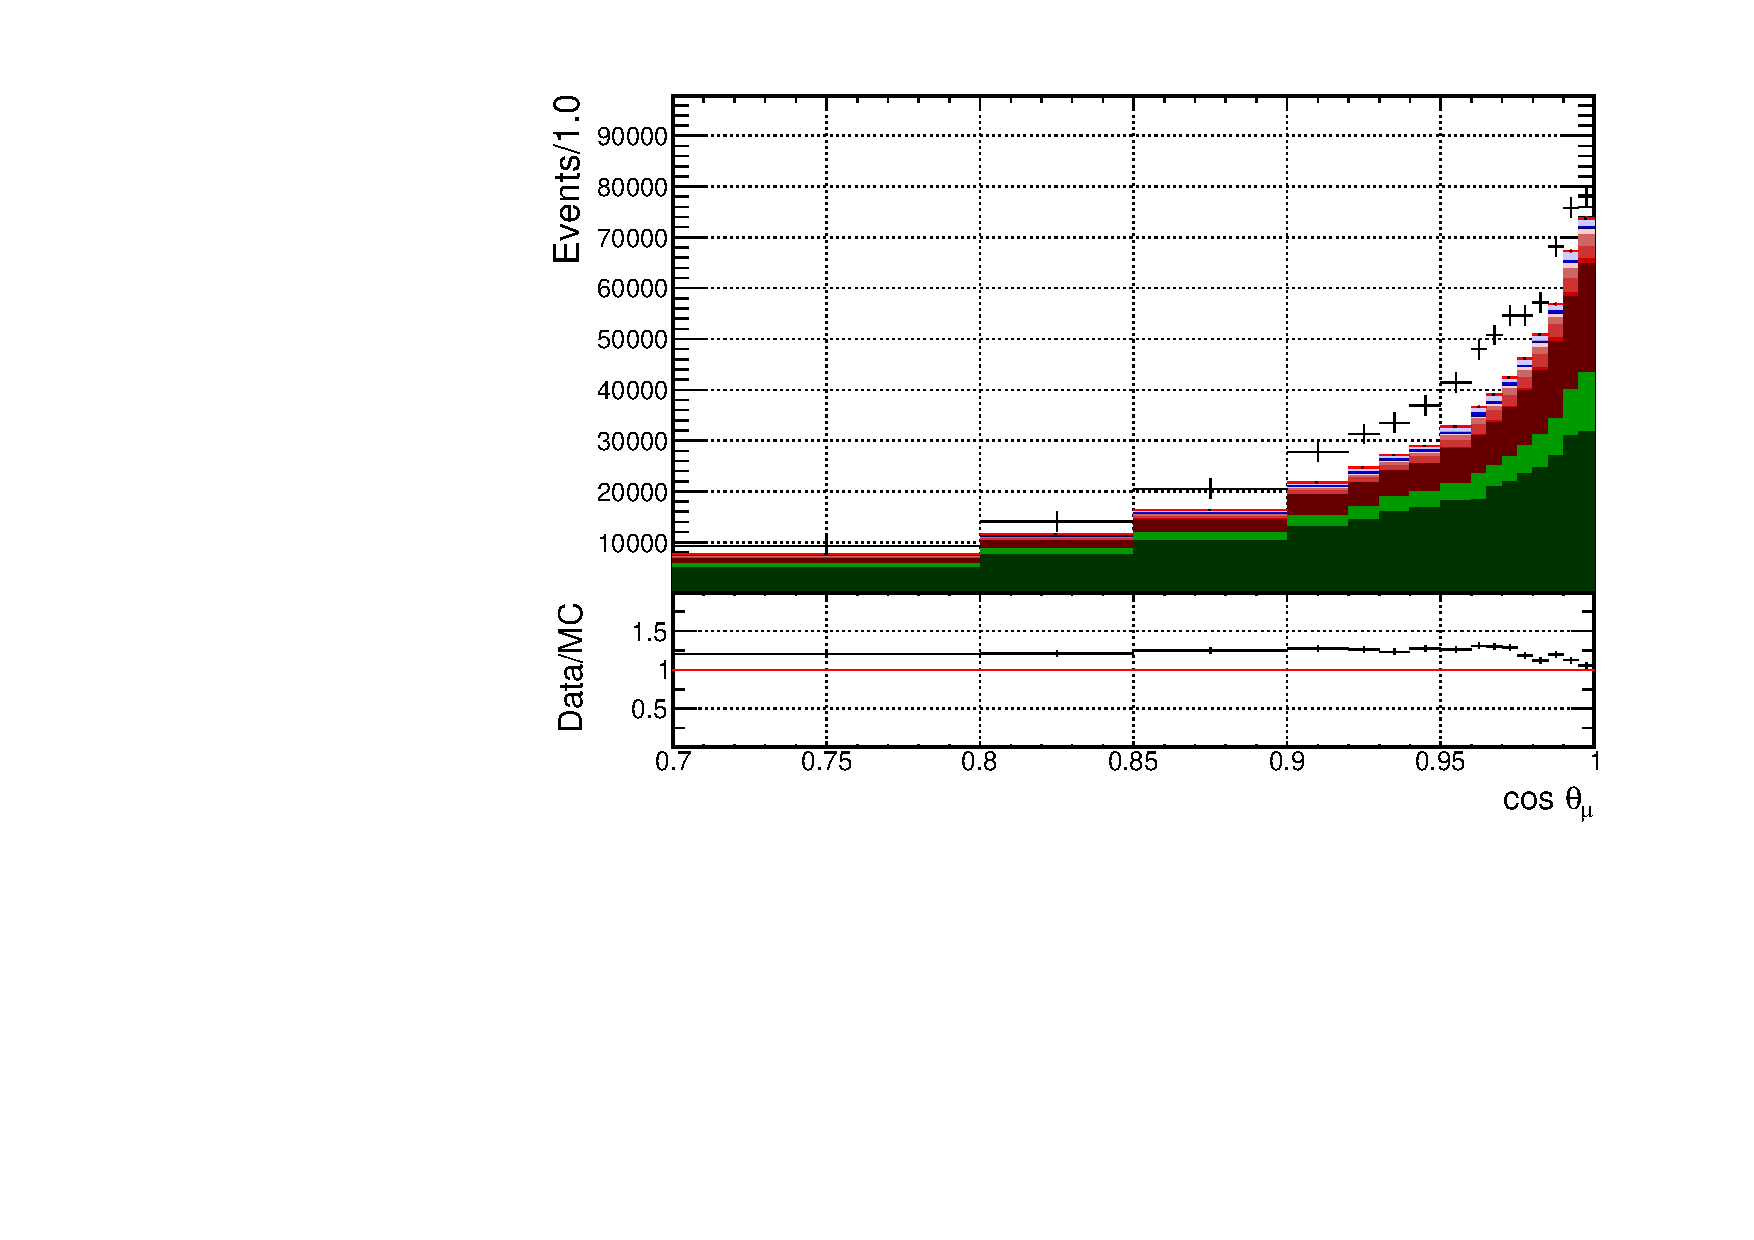
\includegraphics[width=0.95\linewidth]{figs/FGD2_anti-numuCC_0pi_t}
  \caption{FGD2 RHC $\bar{\nu_{\mu}}$ 0$\pi$}
  \label{fig:tstack_FGD2_anti-numuCC_0pi}
\end{subfigure}
\begin{subfigure}{.32\textwidth}
  \centering
  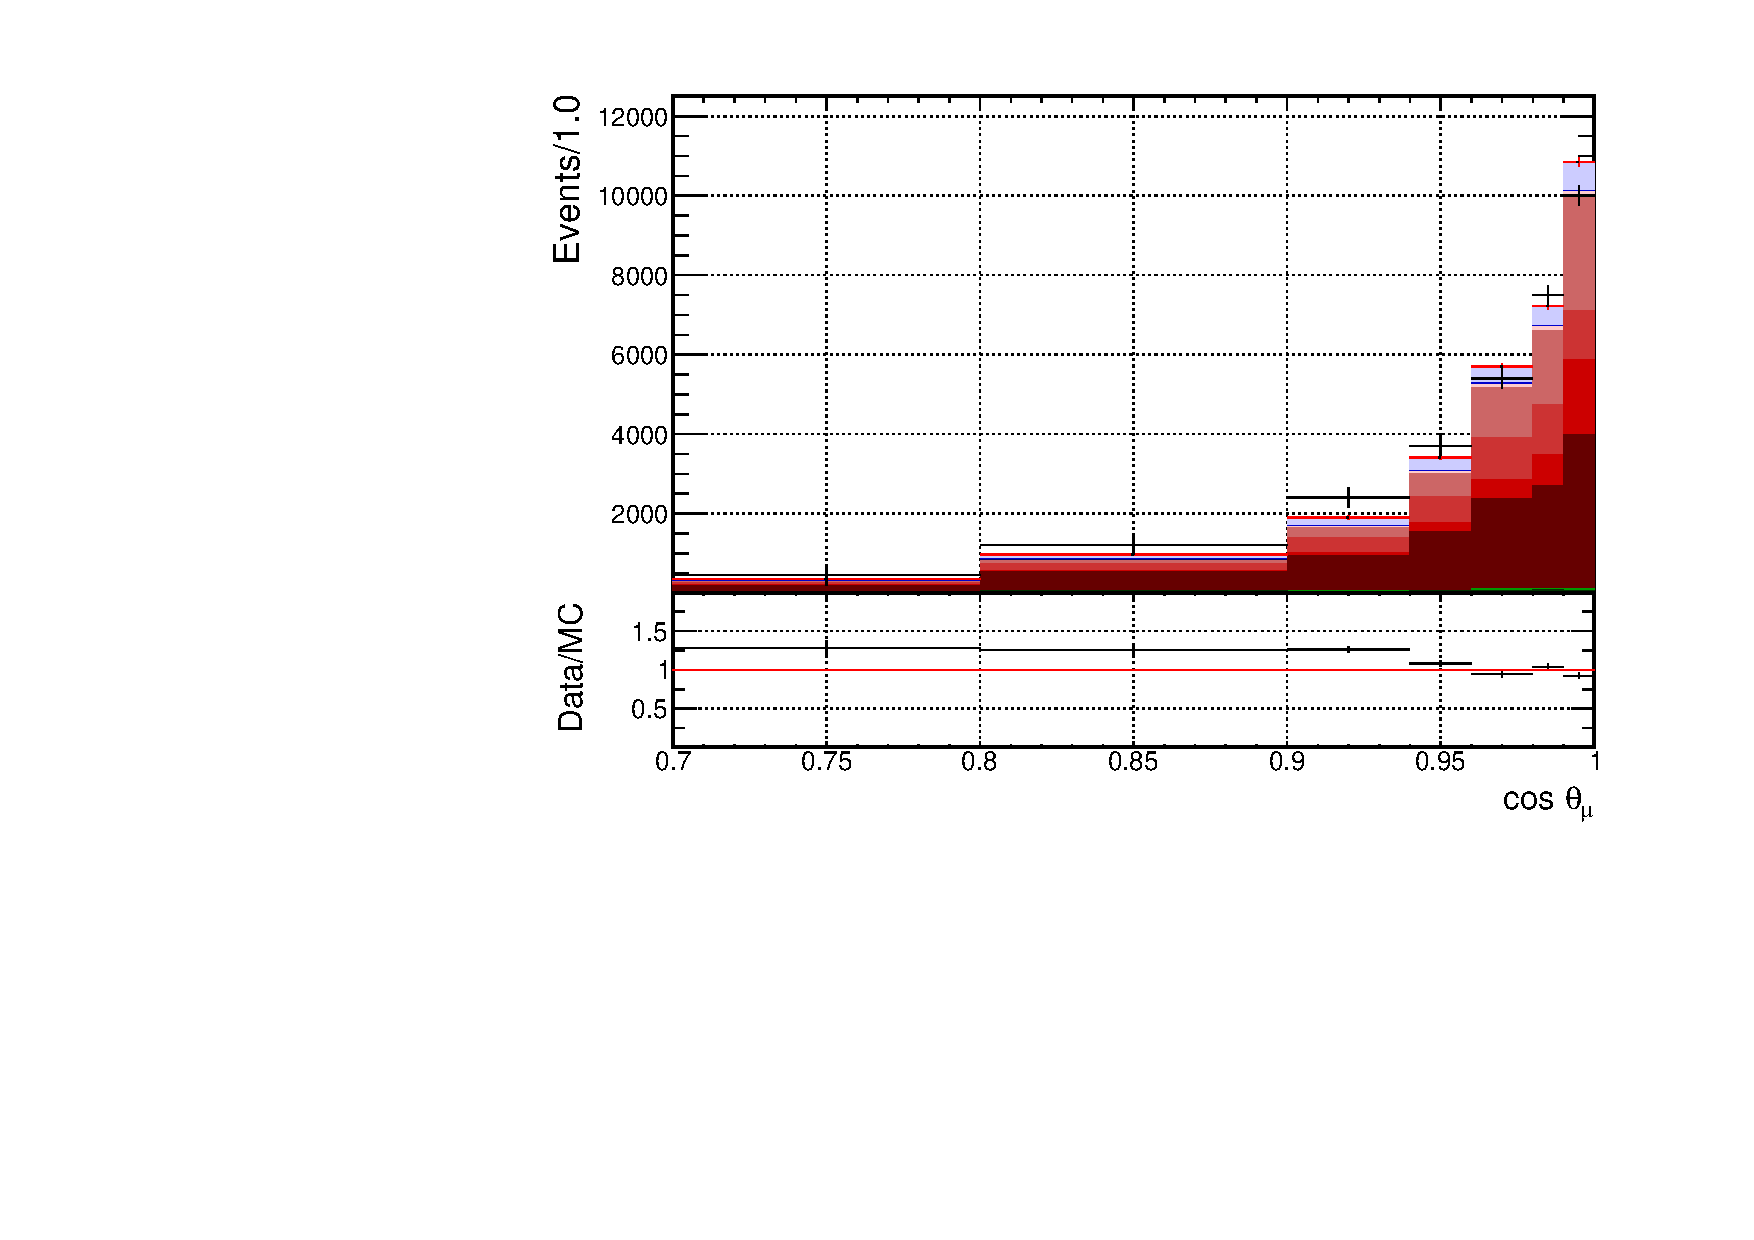
\includegraphics[width=0.95\linewidth]{figs/FGD2_anti-numuCC_1pi_t}
  \caption{FGD2 RHC $\bar{\nu_{\mu}}$ 1$\pi$}
  \label{fig:tstack_tstack_FGD2_anti-numuCC_1pi}
\end{subfigure}
\begin{subfigure}{.32\textwidth}
  \centering
  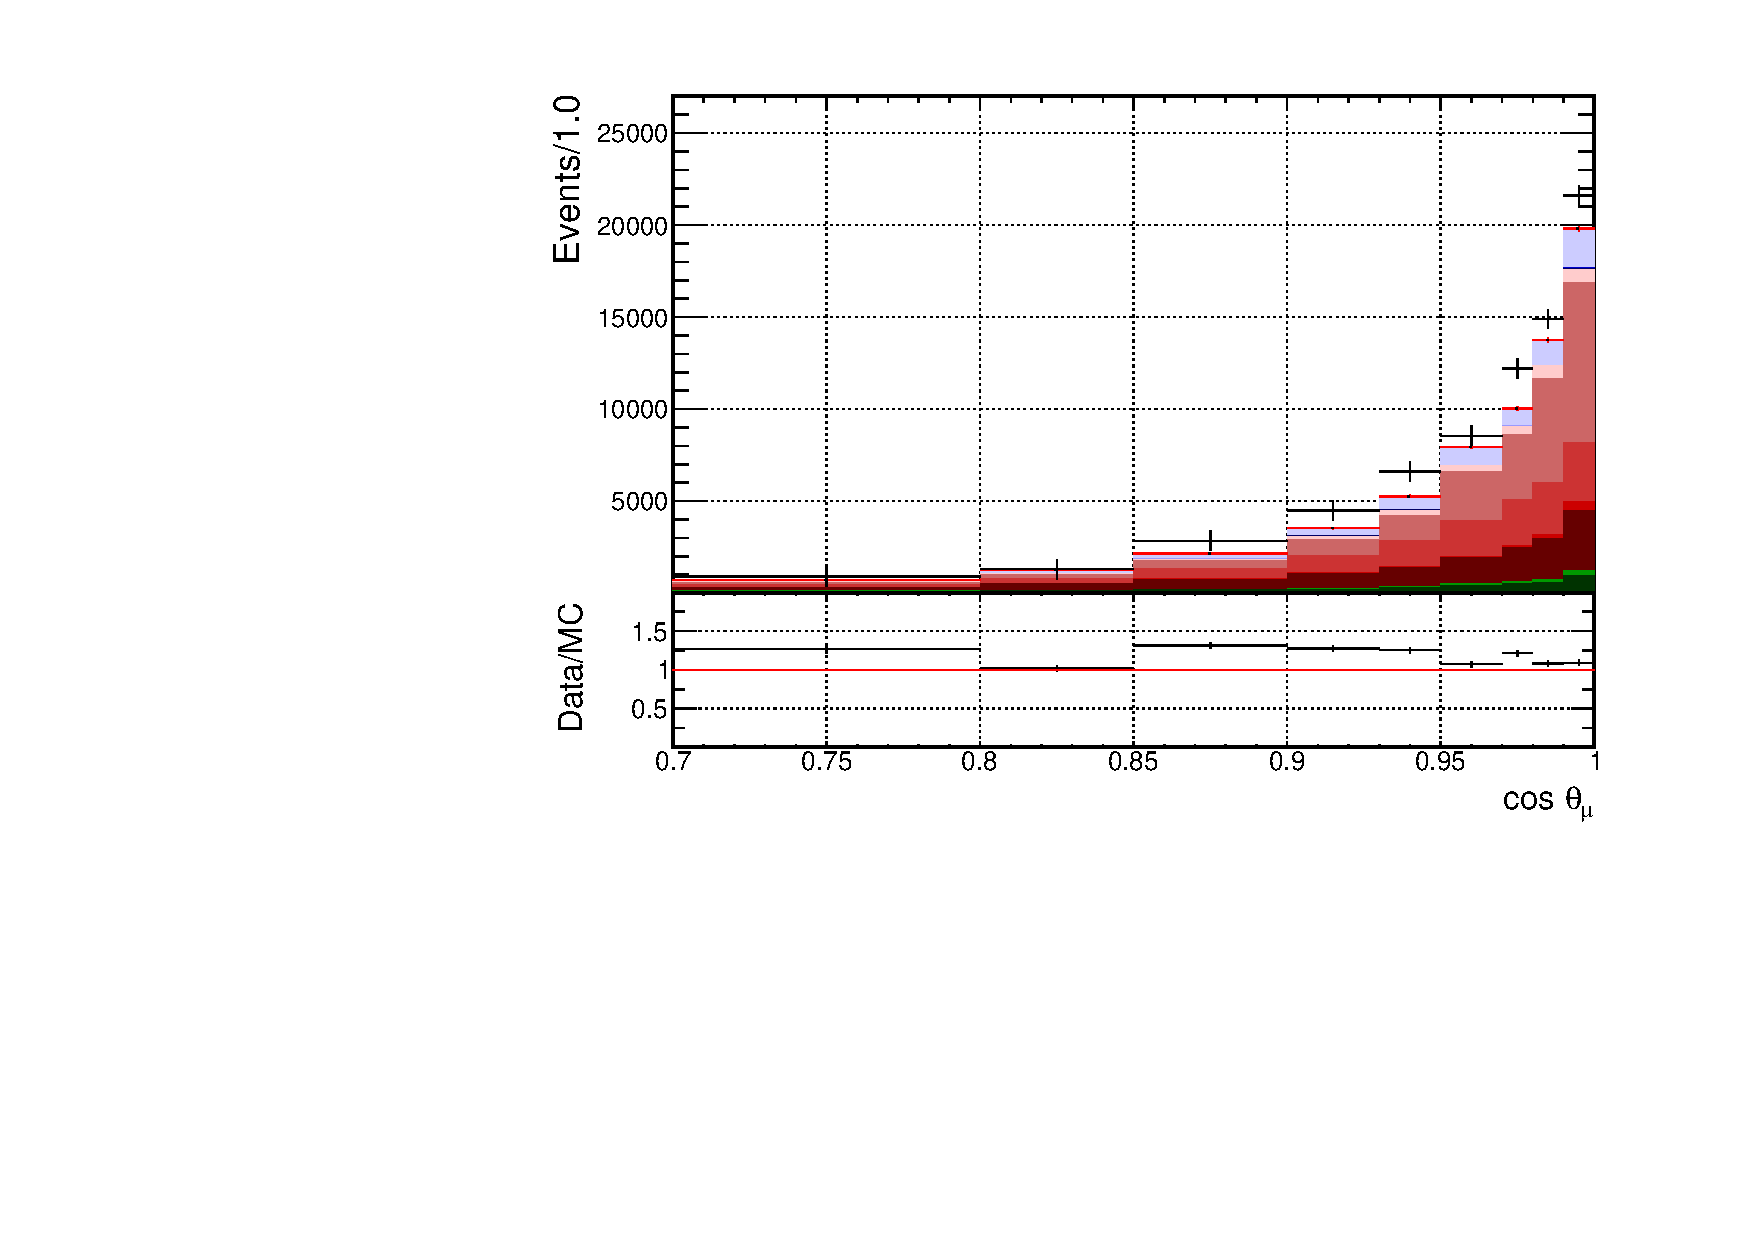
\includegraphics[width=0.95\linewidth]{figs/FGD2_anti-numuCC_other_t}
  \caption{FGD2 RHC $\bar{\nu_{\mu}}$ Other}
  \label{fig:tstack_FGD2_anti-numuCC_other}
\end{subfigure}
\begin{subfigure}{.32\textwidth}
  \centering
  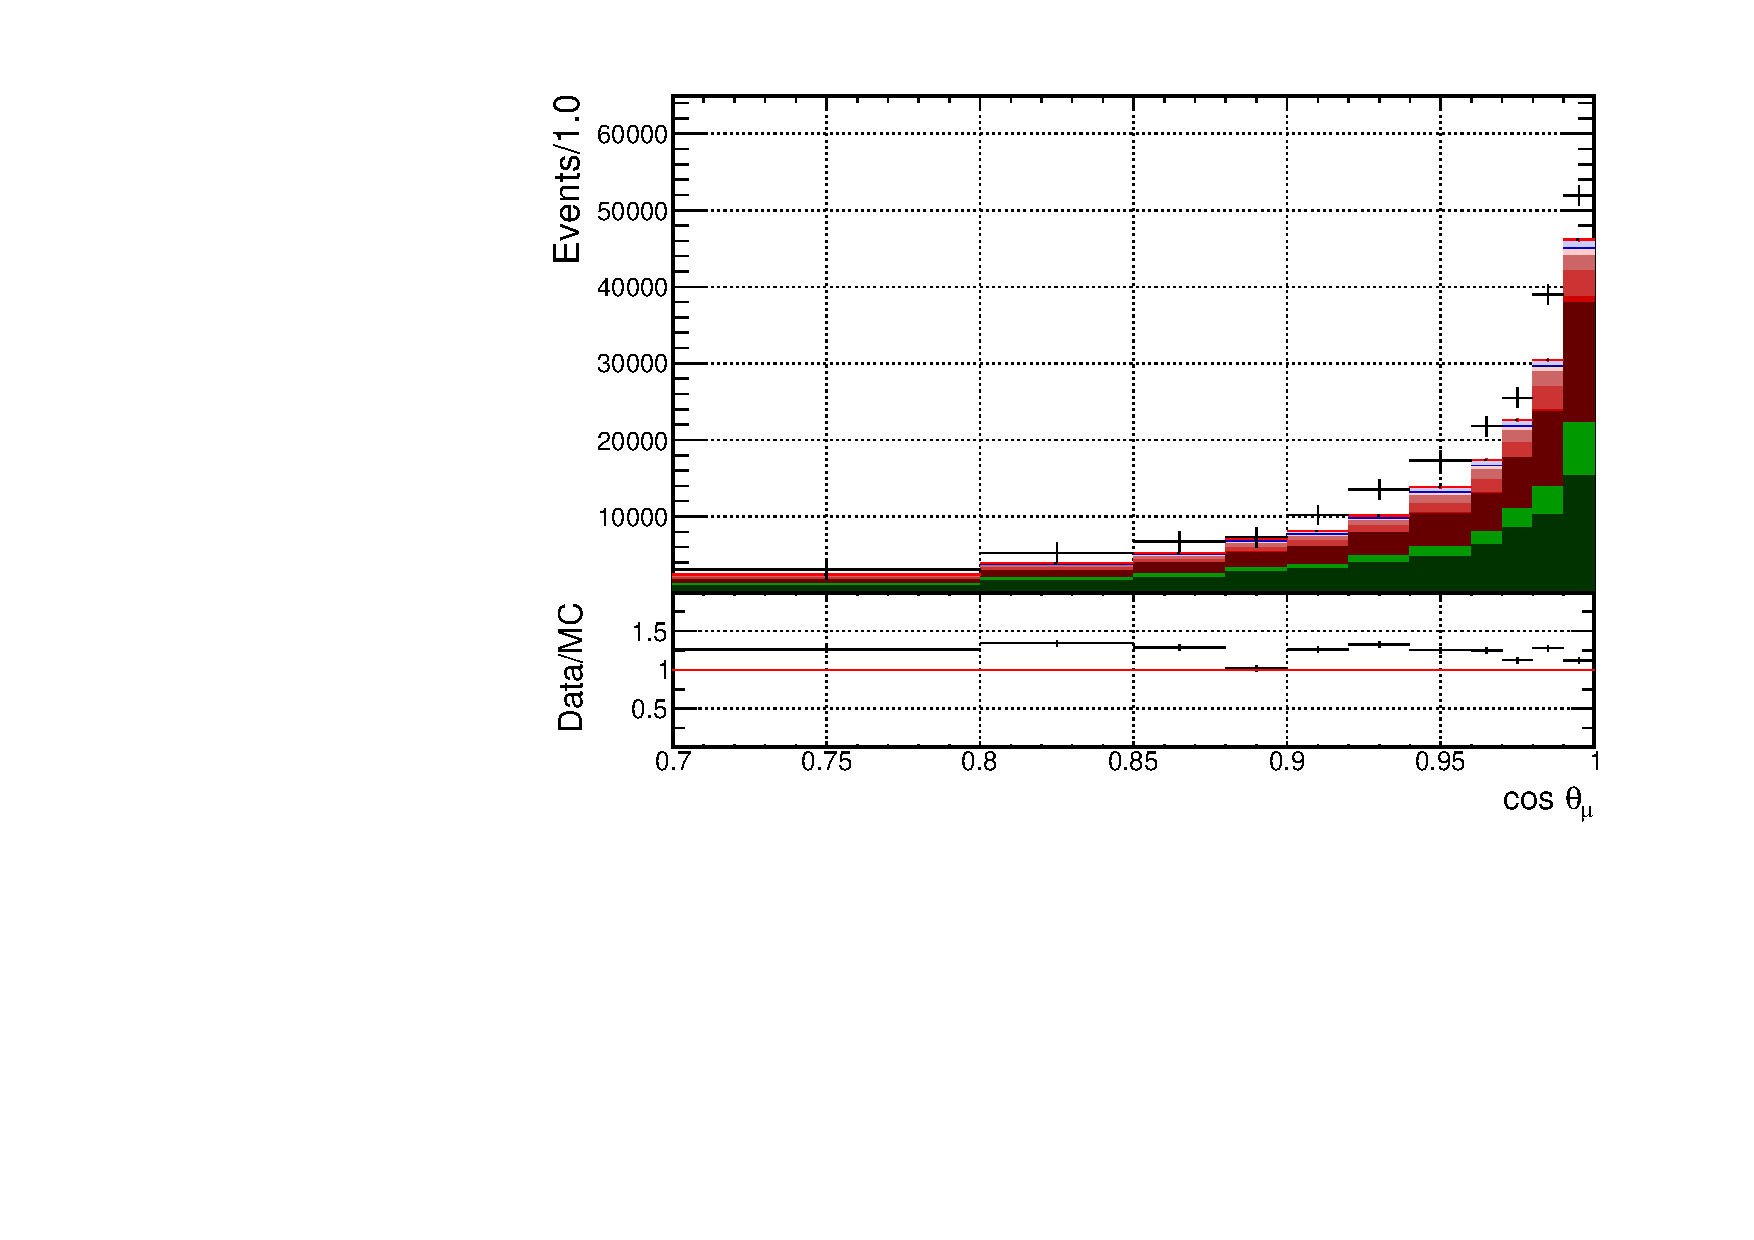
\includegraphics[width=0.95\linewidth]{figs/FGD1_NuMuBkg_CC0pi_in_AntiNu_Mode_t}
  \caption{FGD1 RHC $\nu_{\mu}$ 0$\pi$}
  \label{fig:tstack_FGD1_NuMuBkg_CC0pi_in_AntiNu_Mode}
\end{subfigure}
\begin{subfigure}{.32\textwidth}
  \centering
  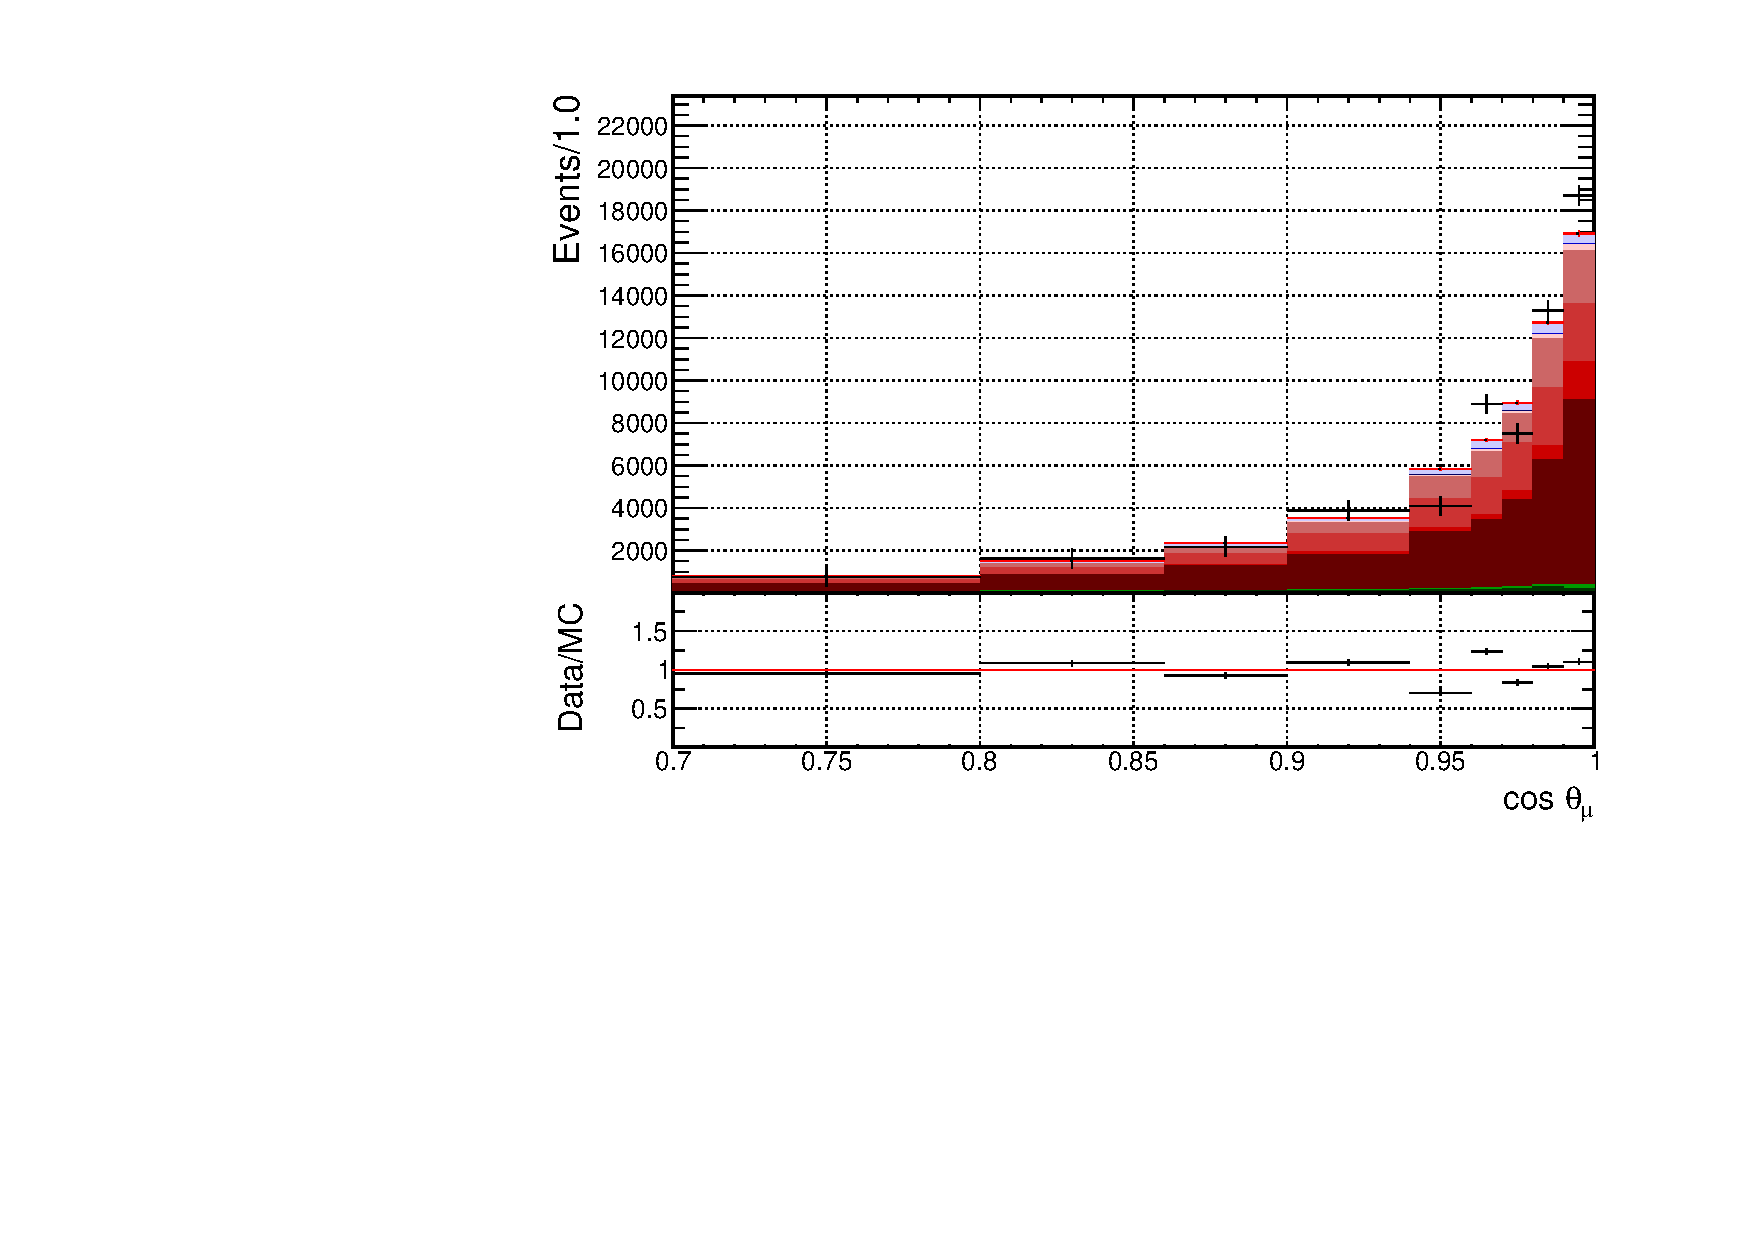
\includegraphics[width=0.95\linewidth]{figs/FGD1_NuMuBkg_CC1pi_in_AntiNu_Mode_t}
  \caption{FGD1 RHC $\nu_{\mu}$ 1$\pi$}
  \label{fig:tstack_FGD1_NuMuBkg_CC1pi_in_AntiNu_Mode}
\end{subfigure}
\begin{subfigure}{.32\textwidth}
  \centering
  \includegraphics[width=0.95\linewidth]{figs/FGD1_NuMuBkg_CCOther_in_AntiNu_Mode_t}
  \caption{FGD1 RHC $\nu_{\mu}$ Other}
  \label{fig:tstack_FGD1_NuMuBkg_CCOther_in_AntiNu_Mode}
\end{subfigure}
\begin{subfigure}{.32\textwidth}
  \centering
  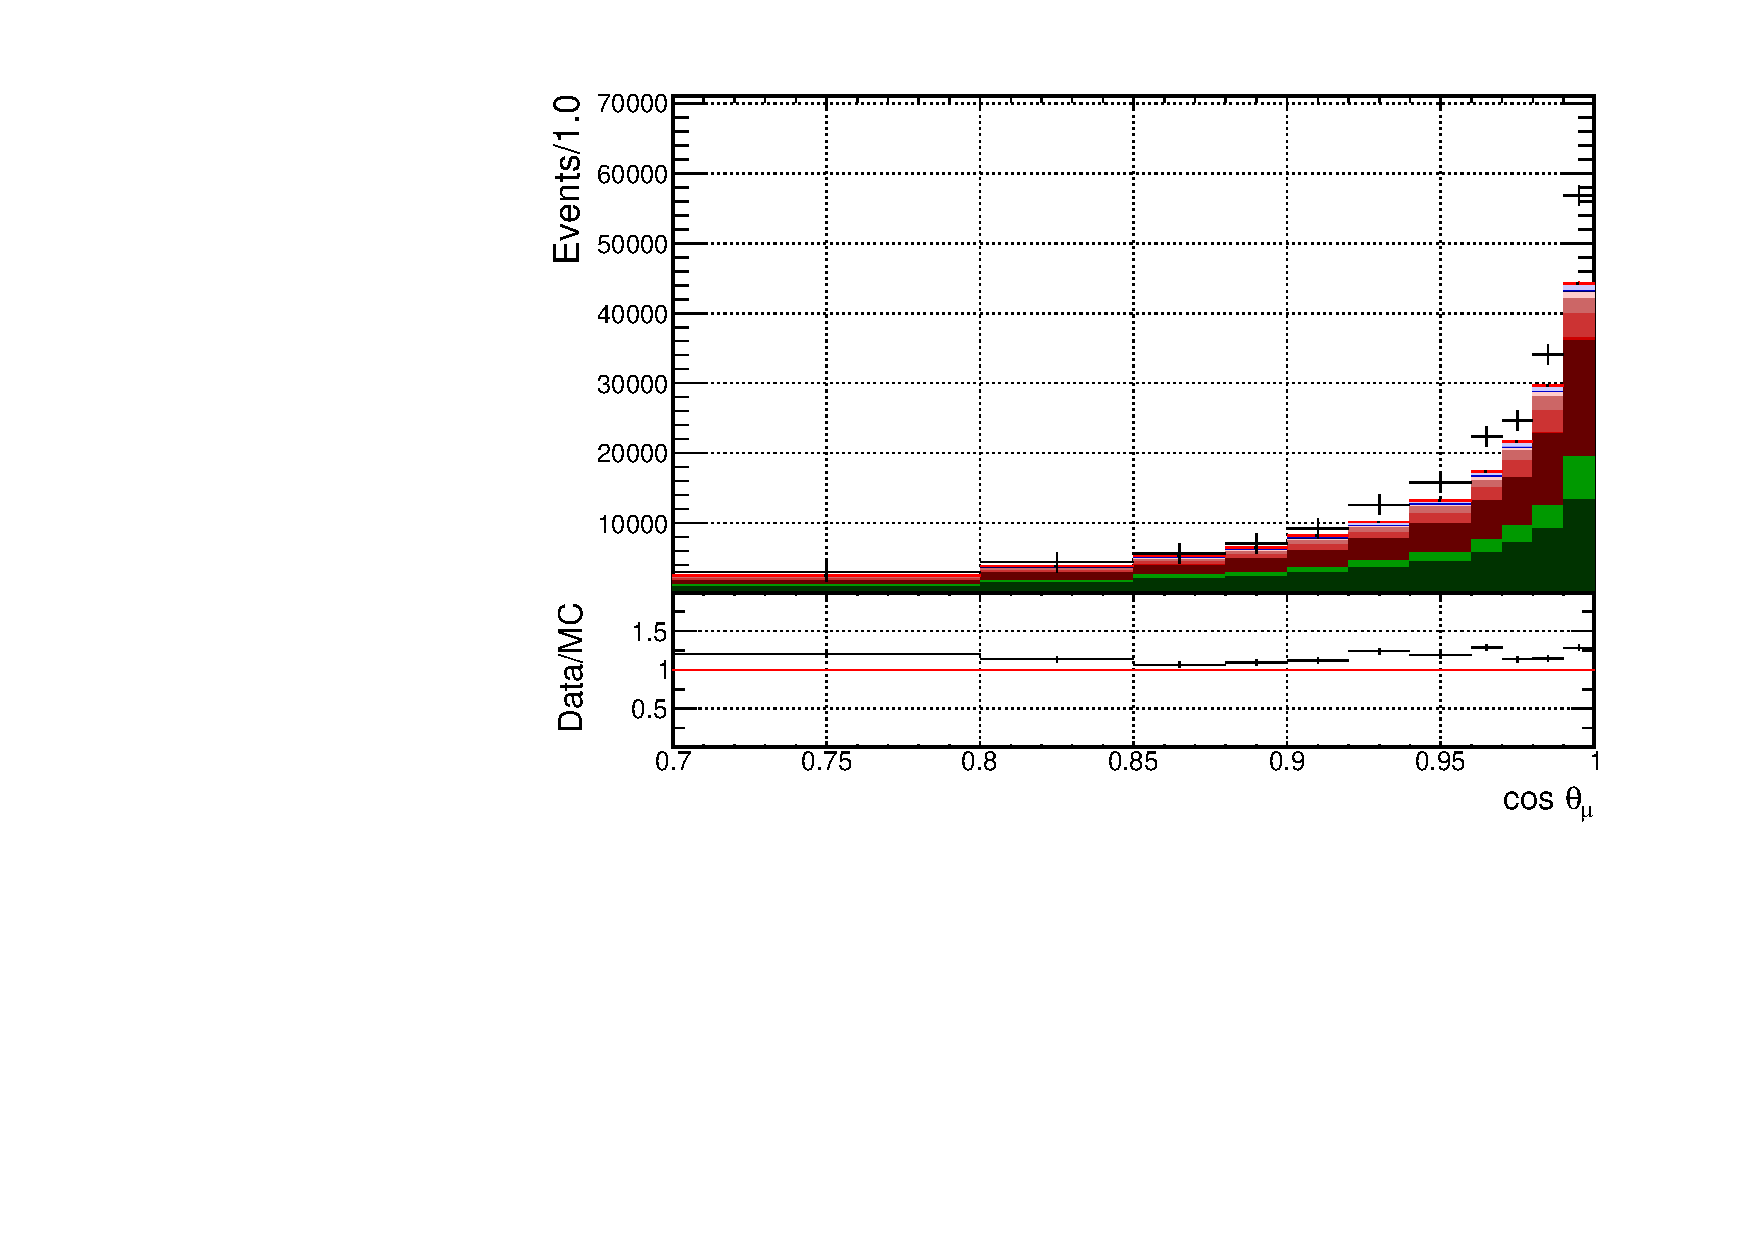
\includegraphics[width=0.95\linewidth]{figs/FGD2_NuMuBkg_CC0pi_in_AntiNu_Mode_t}
  \caption{FGD2 RHC $\nu_{\mu}$ 0$\pi$}
  \label{fig:tstack_FGD2_NuMuBkg_CC0pi_in_AntiNu_Mode}
\end{subfigure}
\begin{subfigure}{.32\textwidth}
  \centering
  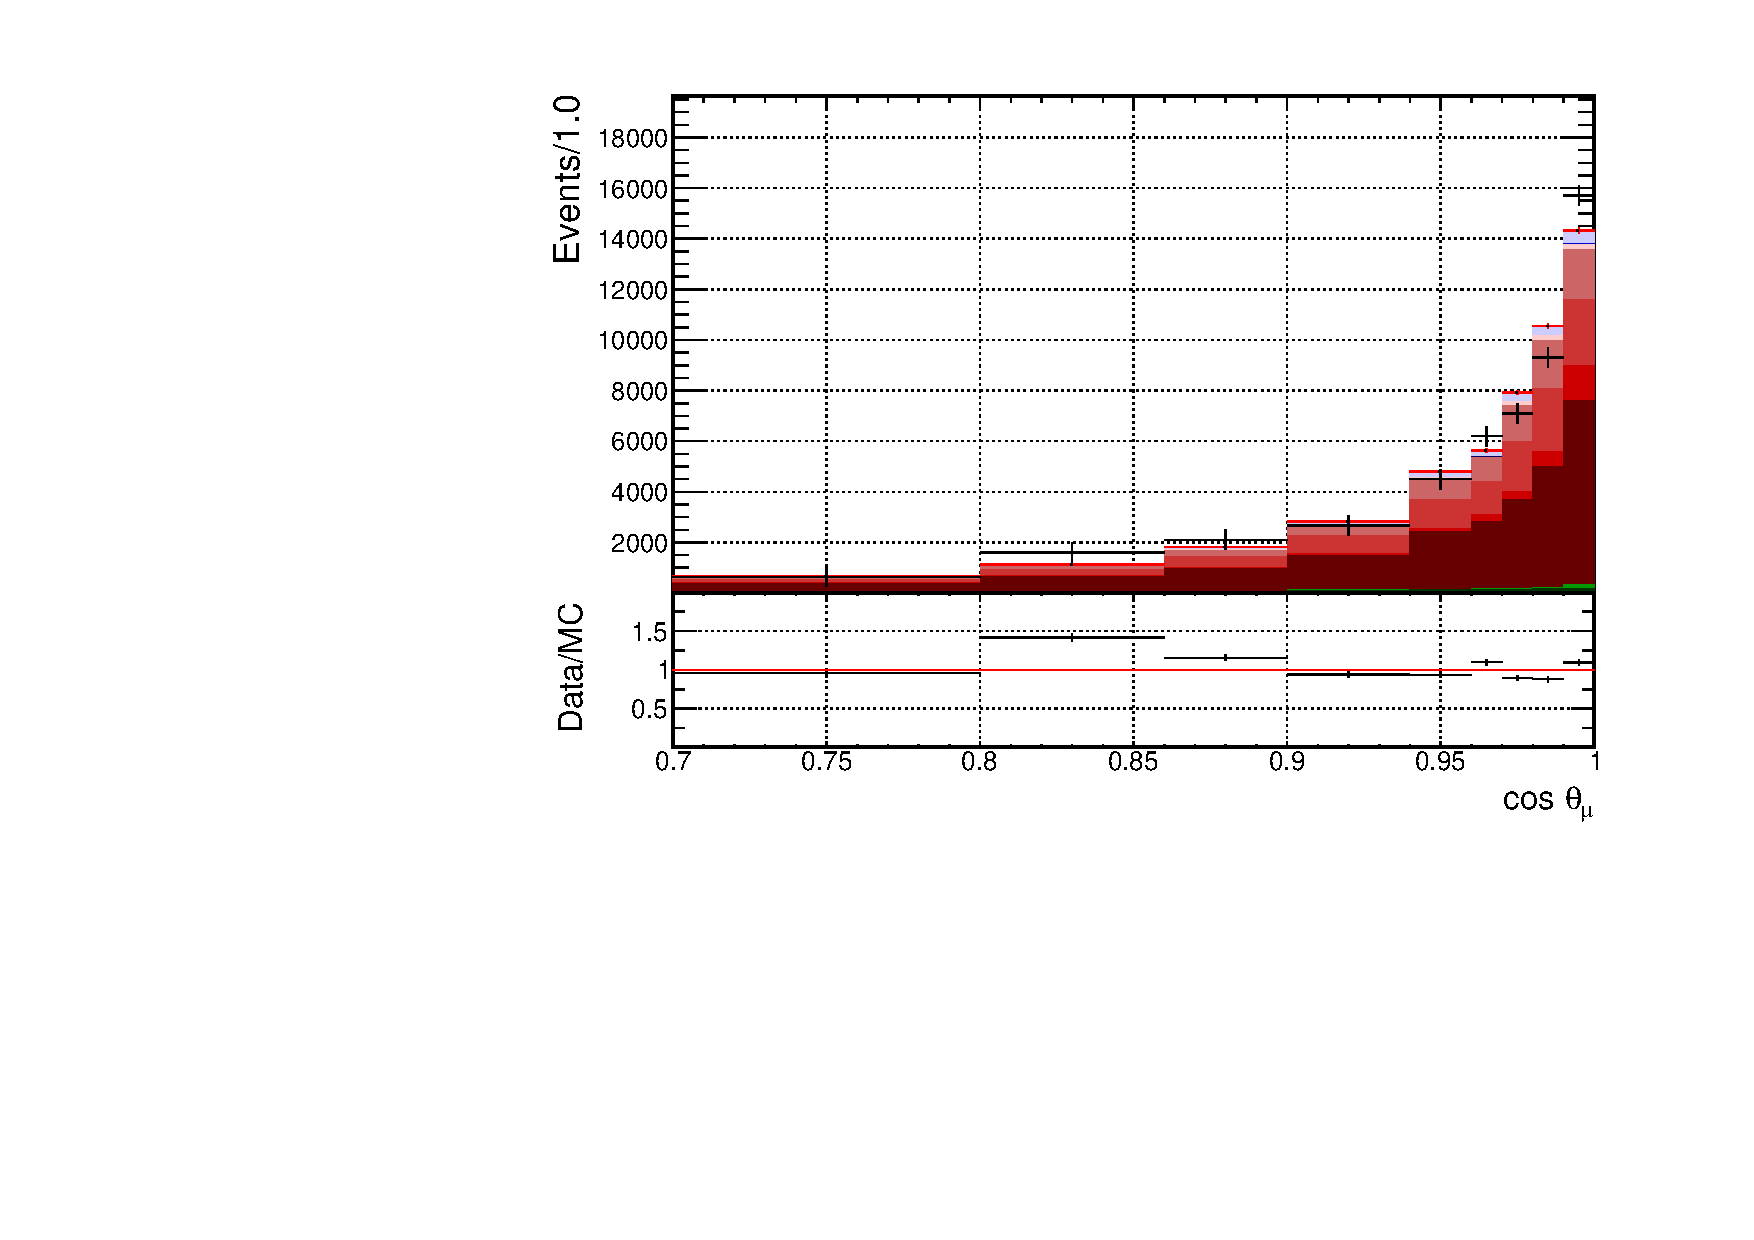
\includegraphics[width=0.95\linewidth]{figs/FGD2_NuMuBkg_CC1pi_in_AntiNu_Mode_t}
  \caption{FGD2 RHC $\nu_{\mu}$ 1$\pi$}
  \label{fig:tstack_FGD2_NuMuBkg_CC1pi_in_AntiNu_Mode}
\end{subfigure}
\begin{subfigure}{.32\textwidth}
  \centering
  \includegraphics[width=0.95\linewidth]{figs/FGD2_NuMuBkg_CCOther_in_AntiNu_Mode_t}
  \caption{FGD2 RHC $\nu_{\mu}$ Other}
  \label{fig:tstack_FGD2_NuMuBkg_CCOther_in_AntiNu_Mode}
\end{subfigure}
\caption{$cos\theta_{\mu}$ projections of data and nominal MC broken down by interaction mode.}
\label{fig:pstack}
\end{figure}

\section{Log Likelihood Scans}\label{sec:llhscan}

The FHC $\nu$ and RHC $\bar{\nu}$ CC 0$\pi$ samples are dominated by the target interaction modes CCQE and 2p2h. However, for RHC $\nu$, there is a large contamination of CC 1$\pi$ events. The FHC $\nu$ and RHC $\bar{\nu}$ CC 1$\pi$ samples are dominated by the target interaction modes CC 1$\pi$, CC coherent, and CC mult-$\pi$. For RHC $\nu$ the 1$\pi$ sample has a significant number of CC DIS events. The CC Other samples are populated by mainly the target interaction modes CC DIS, CC mult-$\pi$, and CC miscellaneous, but with a significant number CC $1\pi$ and CC coherent events for FHC $\nu$ and RHC $\bar{\nu}$.

\section{Parameter Variations}\label{sec:sigvar}
\section{Asimov Fit}\label{sec:asimov}
\section{Prior Predictions}
\section{Data Fit}\label{sec:datafit}
\section{Posterior Predictions}\label{sec:postpred}
\section{Finer Fit and Detector Binning}\label{sec:newbin}
\subsection{Asimov Fits}
\subsection{Data Fits}
\subsection{Posterior Predictions}
\section{Oscillation Parameter Sensitivity}

\newpage
